% \documentclass[handout]{beamer}
\documentclass{beamer}
\mode<presentation>
{
  \usetheme{Warsaw}
  % \setbeamercovered{transparent}
  \useoutertheme{infolines}

}

\usepackage[english]{babel}
\usepackage[utf8]{inputenc}
\usepackage{wrapfig}
\usepackage[T1]{fontenc}
\usepackage{float}
\usepackage{multicol}
\usepackage{blindtext}
\usepackage{mwe}

\setlength{\multicolsep}{4.0pt plus 1.0pt minus 1.0pt}

\definecolor{nord1}{RGB}{46, 52, 64} 
\definecolor{nord2}{RGB}{76, 105, 141} 
\definecolor{nord3}{RGB}{94, 129, 172}
\definecolor{nord4}{RGB}{129, 161, 193} 
\definecolor{nord5}{RGB}{136, 192, 208}  
\definecolor{nord6}{RGB}{163, 190, 140}
\definecolor{nord7}{RGB}{191, 97, 106}
\definecolor{nordred}{RGB}{191, 97, 106}
\definecolor{nordgreen}{RGB}{135, 157, 116}

\setbeamercolor{palette primary}{bg=nord2,fg=white}
\setbeamercolor{palette secondary}{bg=nord3,fg=white}
\setbeamercolor{palette tertiary}{bg=nord4,fg=white}


\setbeamercolor{block title}{bg=nord2,fg=white}

\setbeamercolor{itemize item}{fg=nord3}
\setbeamercolor{itemize subitem}{fg=nord4}
\setbeamercolor{itemize subsubitem}{fg=nord5}

\setbeamertemplate{itemize item}[square]
\setbeamertemplate{itemize subitem}[circle]
\setbeamertemplate{itemize subsubitem}[triangle]
\setbeamerfont{bibliography item}{size=\scriptsize}
\setbeamerfont{bibliography entry author}{size=\scriptsize}
\setbeamerfont{bibliography entry title}{size=\scriptsize}
\setbeamerfont{bibliography entry location}{size=\tiny}
\setbeamerfont{bibliography entry note}{size=\tiny}

\usecolortheme[named=nord2]{structure}
\setbeamertemplate{bibliography item}{\insertbiblabel}
\title[] {PiCnIc pipeline for Lung Adenocarcinoma}

% \subtitle
% {Presentation Subtitle} % (optional)

\author[] {Davide Cozzi, 829827 - 
  Mattia Sgrò, 829474}


\institute[] {Dipartimento di Informatica, Sistemistica e Comunicazione
  (DISCo)\\
  Università degli Studi di Milano Bicocca}

\date[] {}

\subject{Presentation}
\pgfdeclareimage[height=0.5cm]{university-logo}{img/logo_unimib.pdf}
\logo{\pgfuseimage{university-logo}}

\AtBeginSection[]
{
  \begin{frame}<beamer>{Outline}
    \tableofcontents[currentsection, currentsubsection]
  \end{frame}
}


% If you wish to uncover everything in a step-wise fashion, uncomment
% the following command: 

% \beamerdefaultoverlayspecification{<+->}


\begin{document}

\begin{frame}
  \titlepage
\end{frame}

\begin{frame}{Outline}
  \setcounter{tocdepth}{1}
  \tableofcontents
\end{frame}

\section{Lung Adenocarcinoma}
\subsection{PiCnIc Pipeline}
\begin{frame}{The pipeline for LUAD analysis}
  \begin{block}{Aim of the project}
    With this project we intend to built a cancer progression
    model from cross-sectional \textit{\textbf{lung adenocarcinoma}} data, using
    the \textbf{PiCnIc pipeline} \cite{picnic} via the \textbf{R TRONCO library}
    \cite{troncopaper}.  
  \end{block}
  \begin{figure}
    \centering
    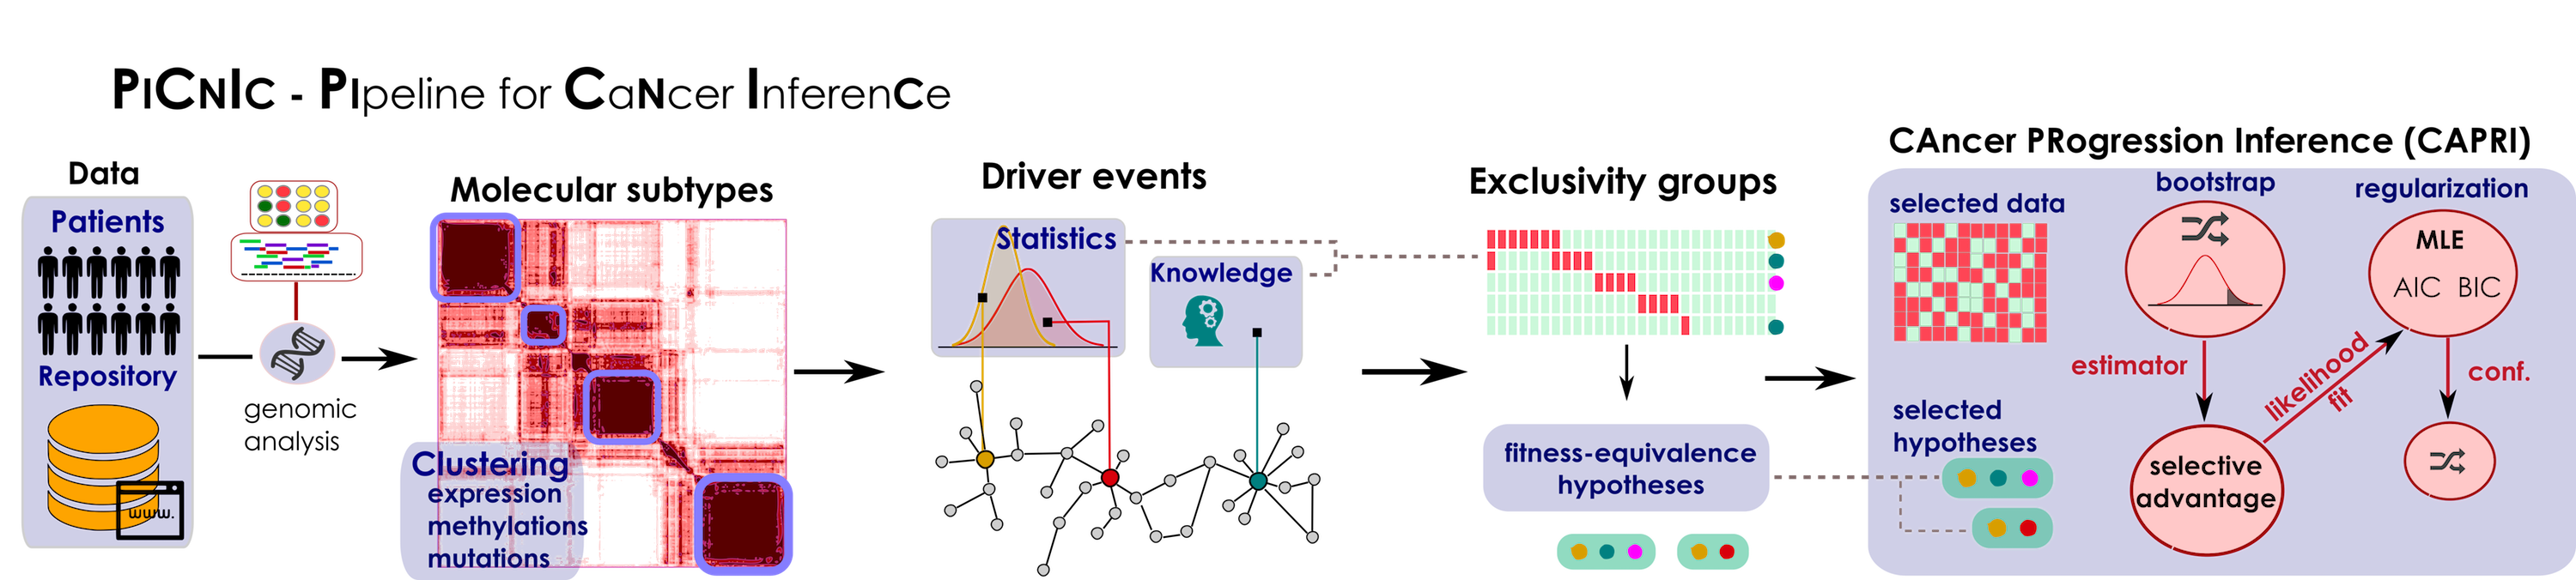
\includegraphics[scale = 1.55]{img/picnic.png}
  \end{figure}
\end{frame}
\subsection{LUAD}
\begin{frame}{Lung Cancer}
  \begin{block}{Histological classification of lung cancer \cite{lungimage}}
    \begin{itemize}
      \item Lung cancer histological types
      \item Location of the tumours and cell origins
    \end{itemize}       
  \end{block}
  \pause
  \begin{figure}
    \centering
    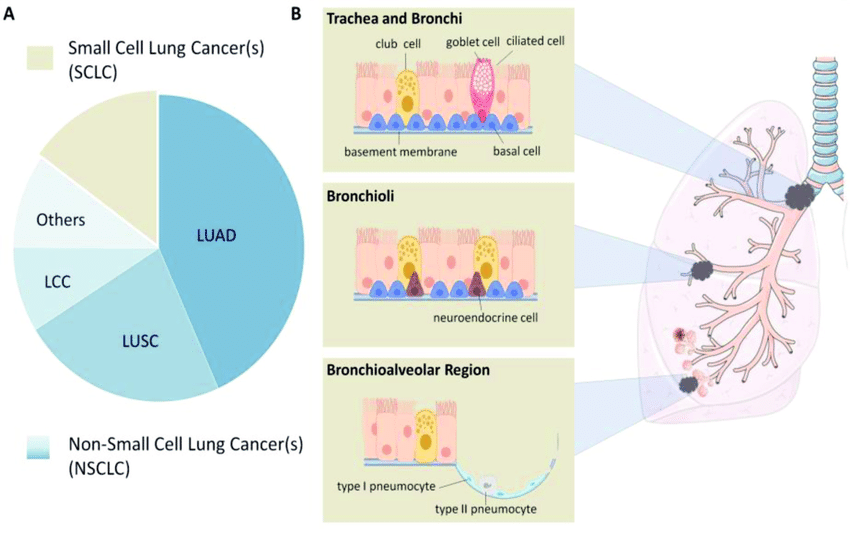
\includegraphics[scale = 0.21]{img/Histological_Lung_Cancer.png}
  \end{figure}
\end{frame}
\begin{frame}{Lung Adenocarcinoma I}
  \begin{block}{}
    \textbf{Lung adenocarcinoma (\textit{LUAD})} is the most common histological
    type of non-small cell lung cancer (\textit{NSCLC}).\\ 
    Due to the nonspecific early symptoms (that are similar across other forms
    of lung cancer, i.e. persistent cough and shortness of breath), the majority
    of the diagnosed \textit{LUAD} patients are in the middle and late stages,
    with multiple metastases, and have missed the optimal period for treatment
    \cite{luadpot}.  
  \end{block}
  \pause
  \begin{block}{}
    \textbf{Adenocarcinoma} is more common in patients with a history of
    cigarette smoking, and is the most common form of lung cancer in younger
    women and Asian populations. The pathophysiology of adenocarcinoma is
    complicated, but generally follows a histologic progression from cells found
    in healthy lungs to distinctly dysmorphic, or irregular cells
    \cite{luadwiki}.  
  \end{block}
\end{frame}
\begin{frame}{Lung Adenocarcinoma II}
  \begin{block}{}
    \textbf{Adenocarcinoma of the lung is the leading cause of cancer death
      worldwide} \cite{luadmarker}. 
  \end{block}
  \begin{figure}
    \centering
    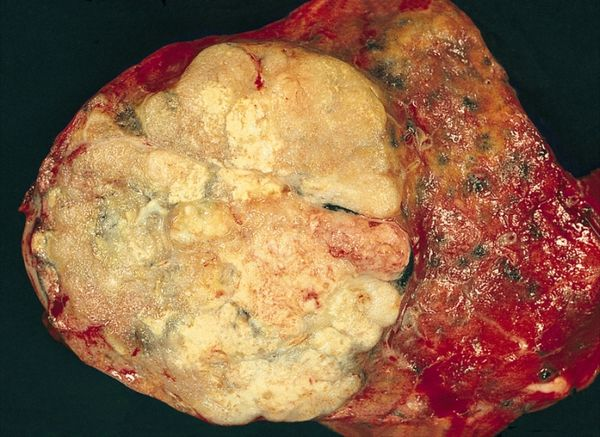
\includegraphics[scale = 0.25]{img/tumor.jpg}
  \end{figure}
\end{frame}
\section{Genes Drivers Selection}
\begin{frame}{Genes Drivers and Pathways I}
  \begin{block}{A first attempt}
    At first we tried to use the results of some software present in the
    literature for the choice of genes drivers \cite{imcdriver}. 
  \end{block}
  \pause
  \begin{table}[H]
    \tiny
    \centering

    \begin{tabular}{|c|c|c|c|c|c|c|}
      \hline {\color{nordgreen}\textit{\textbf{IMC Driver}}} & \textit{SCS}
      & \textit{ACtive Driver} & {\color{nordgreen}\textit\textbf{{MutSigCV}}}
      & \textit{Dawn Rank} & \textit{Driver ML} & \textit{Driver Net} \\
      \hline
      \hline TPS3 & SRGAP3 & NUP155 & C12ORF5 & MAPK3 & EGFR & GRIN2B \\
      \hline LRP1B & PCDHGC5 & LCLAT1 & C16ORF3 & PRKCB & SETD2 & MET \\
      \hline KRAS & ZNFI17 & NEK10 & C19ORF70 & PRKACB & STK11 & RYR2 \\
      \hline TRN & MST1R & SIK31 & C8ORF59 & PRKX & TP53 & PIK3CA \\
      \hline KEAP1 & ZWINT & SOS1 & EGFR & HRAS & RB1 & ADCY8 \\
      \hline$\ldots$ & $\ldots$ & $\ldots$ & $\ldots$ & $\ldots$ & $\ldots$
                                                & $\ldots$ \\
      \hline
    \end{tabular}

  \end{table}
\end{frame}
\begin{frame}{Genes Drivers and Pathways II}
  \begin{block}{Final selection}
    At the end we decided to use the genes drivers and pathways noted in the
    marker paper \cite{luadmarker}. 
  \end{block}
  \begin{figure}
    \centering
    \only<1>
    {%
      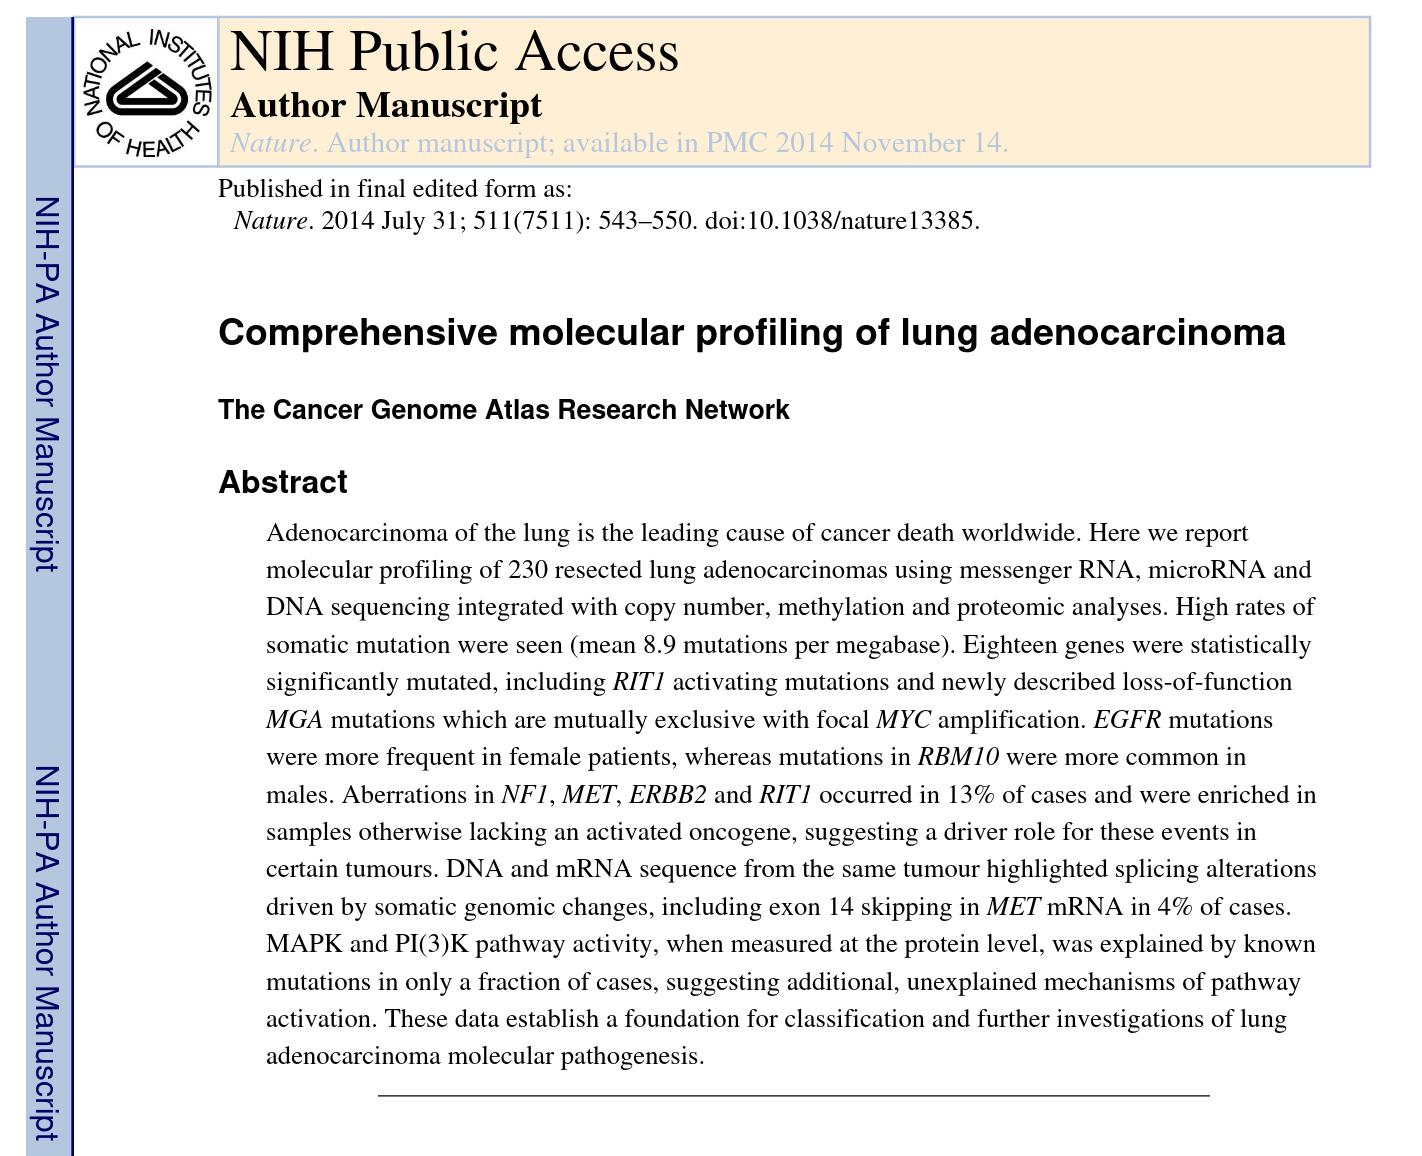
\includegraphics[scale = 0.14]{img/paper.jpg}%
    }%
    \only<2>
    {%
      % 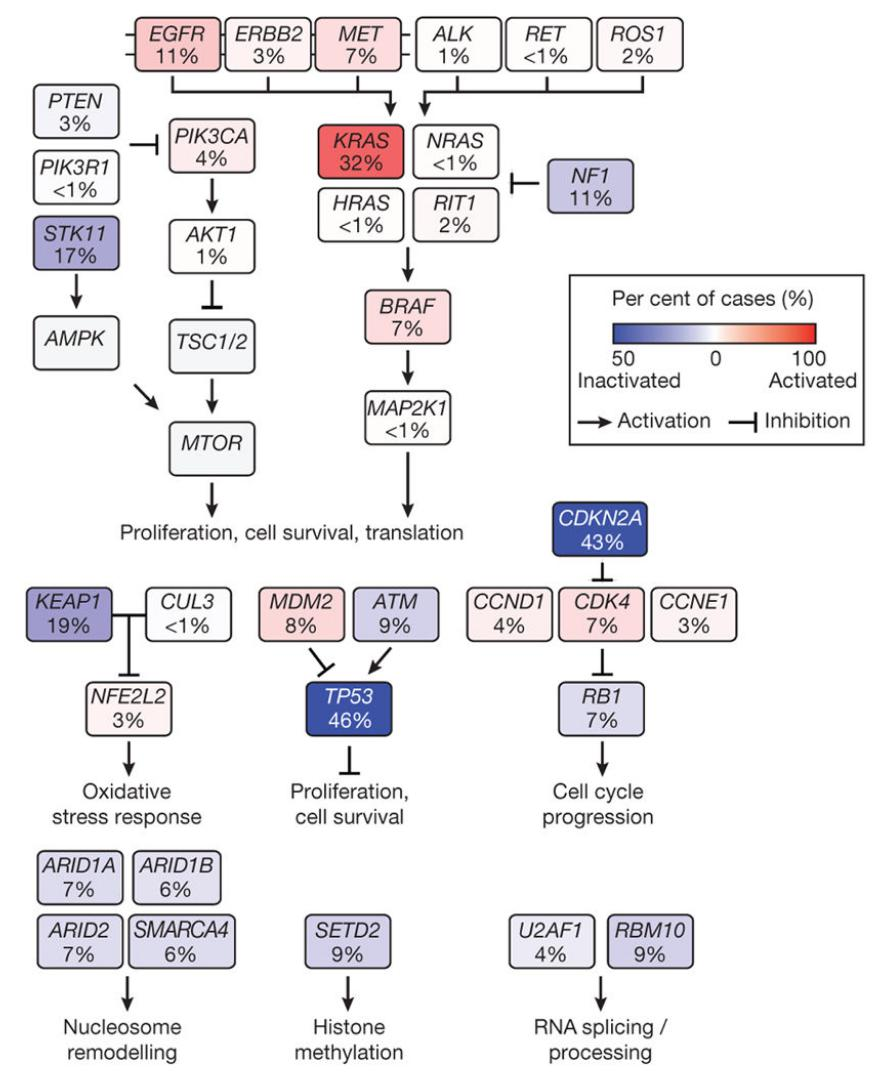
\includegraphics[scale = 0.14]{img/genes.jpg}%
      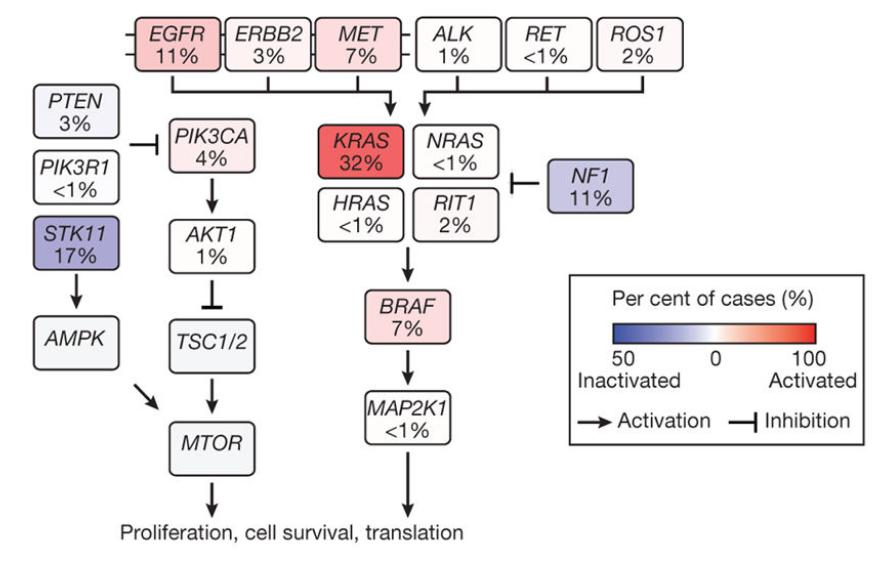
\includegraphics[scale = 0.85]{img/genes1.jpg}%
      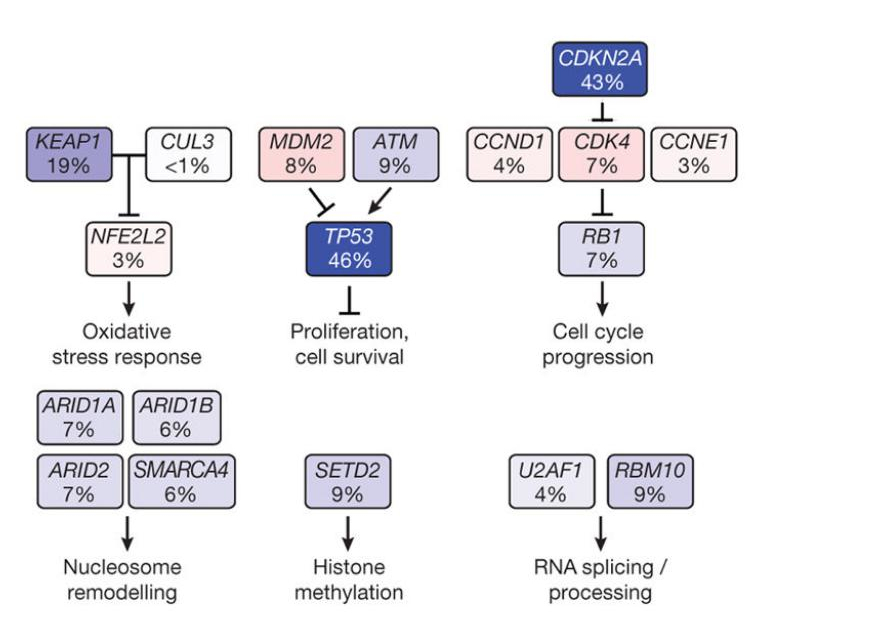
\includegraphics[scale = 0.85]{img/genes2.jpg}%
    }%
  \end{figure}
\end{frame}
\begin{frame}{Genes Drivers and Pathways III}
  \begin{block}{Pathway details using \textbf{WikiPathways R library}
      \cite{wikipw} (although some results are not directly related to
      \textit{LAUD})} 
    \begin{table}[H]
      \footnotesize
      \centering
      \only<1>
      {%
        \begin{tabular}{c||c}
          \textbf{\textit{Short Name}} &\textit{Genes} \\ 
          \hline
          \hline
          \textit{P53} & \textit{TP53 ATM MDM2}\\
          \hline
          \textit{MAPK} & \textit{KRAS NRAS HRAS RIT1 NF1 BRAF MAP2K1}\\
                                       & \textit{EGFR ERBB2 MET ALK RET ROS1} \\ 
          \hline
          \textit{MTOR} & \textit{PTEN PIK3CA PIK3R1 STK11 AKT1 AMPK TSC1
                          TSC2 MTOR}  \\
          \hline
          \textit{OXI} & \textit{KEAP1  CUL3   NFE2L2}\\ 
          \hline
          \textit{PROG} & \textit{CDKN2A CCND1  CDK4   CCNE1  RB1}    \\
          \hline
          \textit{REMO} & \textit{ARID1A  ARID1B  ARID2   SMARCA4} \\
          \hline
          \textit{HIME} & \textit{SETD2} \\
          \hline
          \textit{RNASPL} & \textit{RBM10 U2AF1} \\
          
        \end{tabular}%
      } %
      \only<2>
      {%
        \begin{tabular}{c||c}
          \textbf{\textit{Short Name}} &\textit{First title by WikiPathways} \\ 
          \hline
          \hline
          \textit{P53} & ATM signaling pathway\\
          \hline
          \textit{MAPK} & EGFR tyrosine kinase inhibitor resistance\\ 
          \hline
          \textit{MTOR} & Energy dependent regulation of mTOR by LKB1-AMPK \\
          \hline
          \textit{OXI} & Photodynamic therapy-induced NFE2L2 (NRF2) survival
                         signaling\\ 
          \hline
          \textit{PROG} & G1 to S cell cycle control \\
          \hline
          \textit{REMO} & Tumor suppressor activity of SMARCB1 \\
          \hline
          \textit{HIME} & Histone modifications \\
          \hline
          \textit{RNASPL} & Processing of Capped Intron-Containing Pre-mRNA \\
          
        \end{tabular}%
      } %
      \only<3>
      {%
        \begin{tabular}{c||c}
          \textbf{\textit{Short Name}} &\textit{Second title by WikiPathways}\\ 
          \hline
          \hline
          \textit{P53} & TP53 network\\
          \hline
          \textit{MAPK} & NRF2-ARE regulation\\ 
          \hline
          \textit{MTOR} & Focal adhesion: PI3K-Akt-mTOR-signaling pathway\\
          \hline
          \textit{OXI} & NRF2-ARE regulation\\
          \hline
          \textit{PROG} & Cell cycle\\
          \hline
          \textit{REMO} & Transcriptional regulation by RUNX1\\
          \hline
          \textit{HIME} & \\
          \hline
          \textit{RNASPL} & mRNA processing\\
        \end{tabular}%
      }%
    \end{table}   
  \end{block} 
\end{frame}
\section{Data Import}
\begin{frame}{Data Download}
  \begin{block}{}
    Regarding the data (MAF files, GISTIC files, clinical files and subtypes
    files) we choose to use \textit{GDC portal} and \textit{Firehose}, using the
    \textbf{TCGAbiolinks R  library} \cite{tcgabiolinks} to automate the
    download directly into the source code. 
  \end{block}
  \begin{figure}
    \centering
    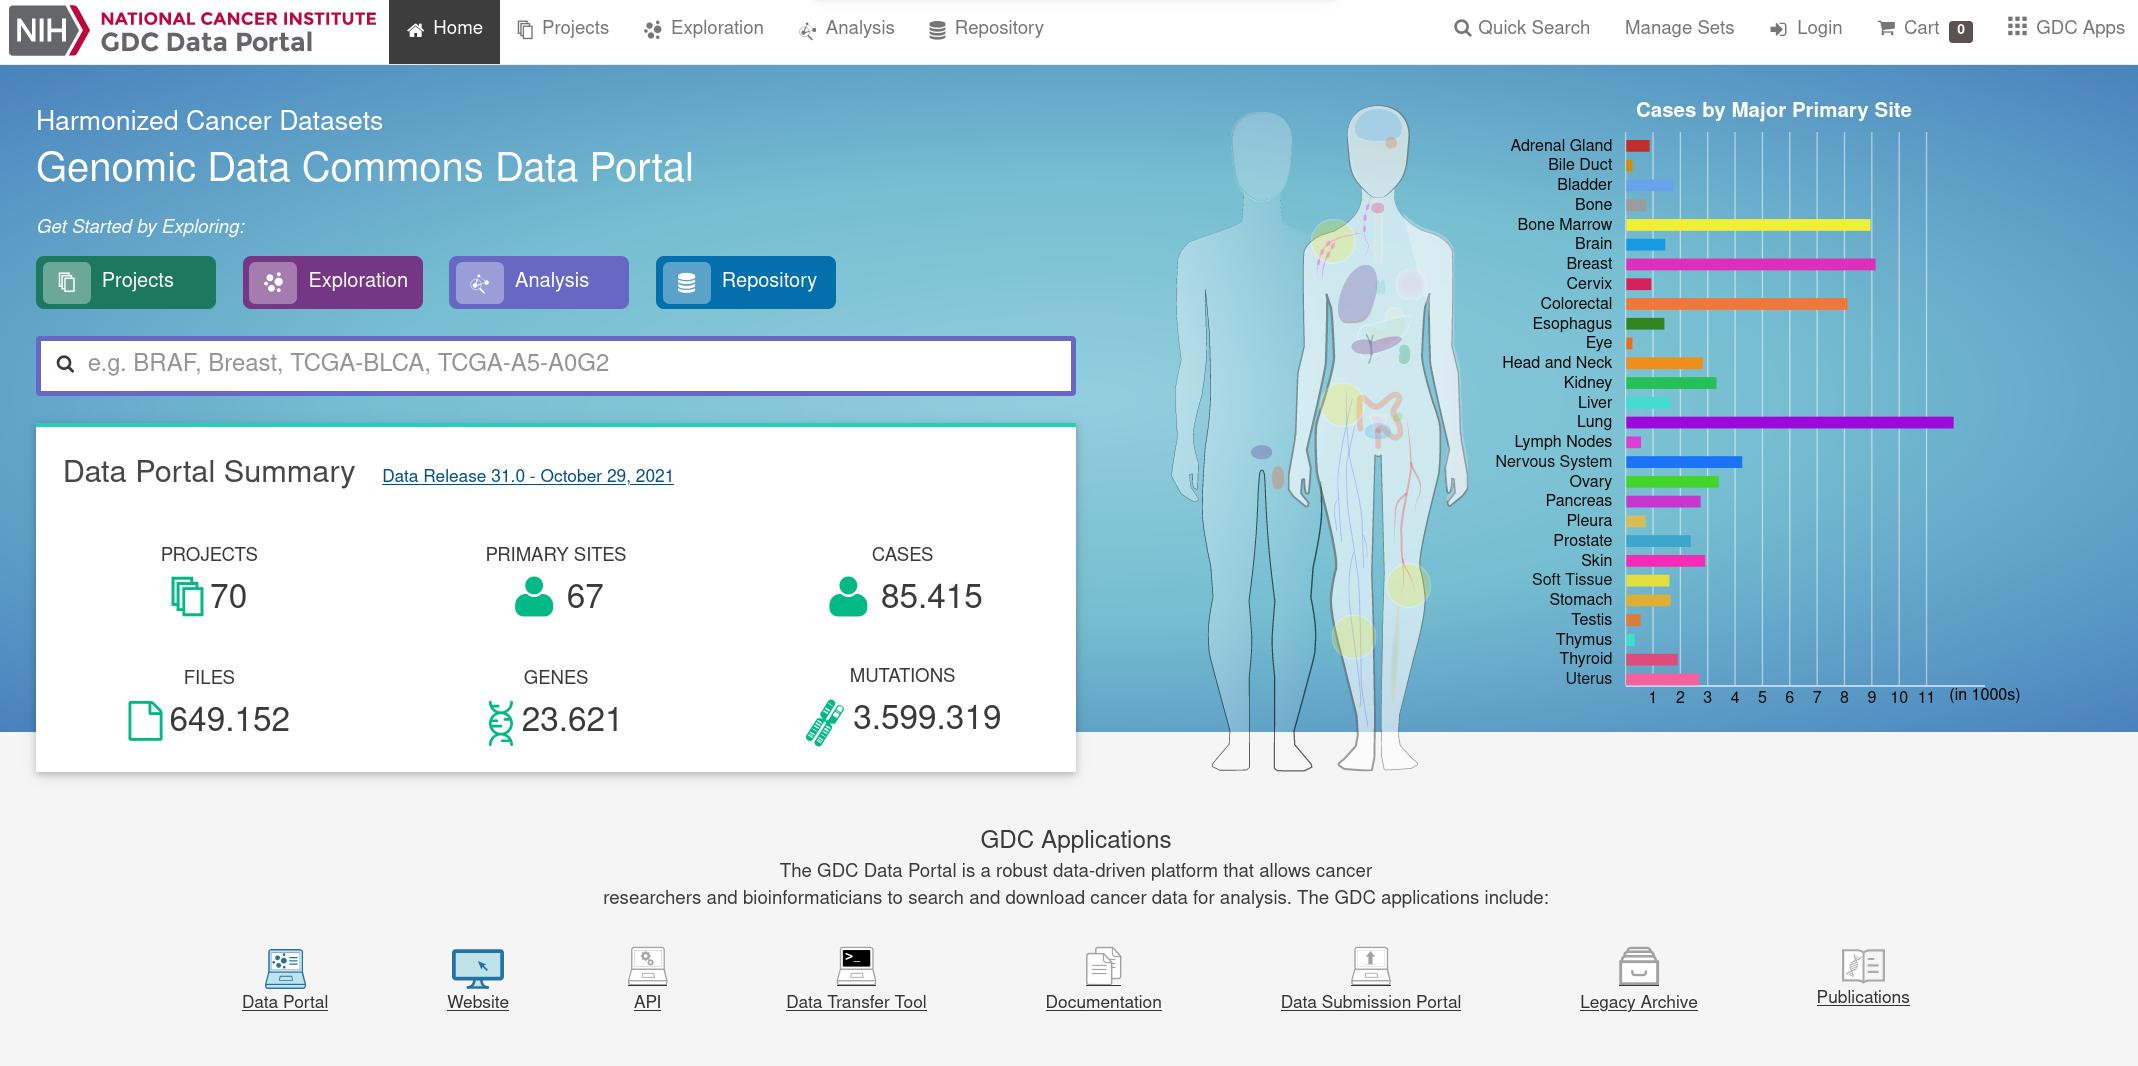
\includegraphics[scale = 0.14]{img/gdc.jpg}
  \end{figure}
\end{frame}
\subsection{MAF}
\begin{frame}{MAF File I}
  \begin{block}{}
    First the MAF file is downloaded, containing the data of the various somatic
    mutations. Important are the column called \textit{Hugo Symbol}, containing
    the code name of the gene, and the \textit{Variant classification} column,
    indicating the type of mutation.  
  \end{block}
  \begin{figure}
    \centering
    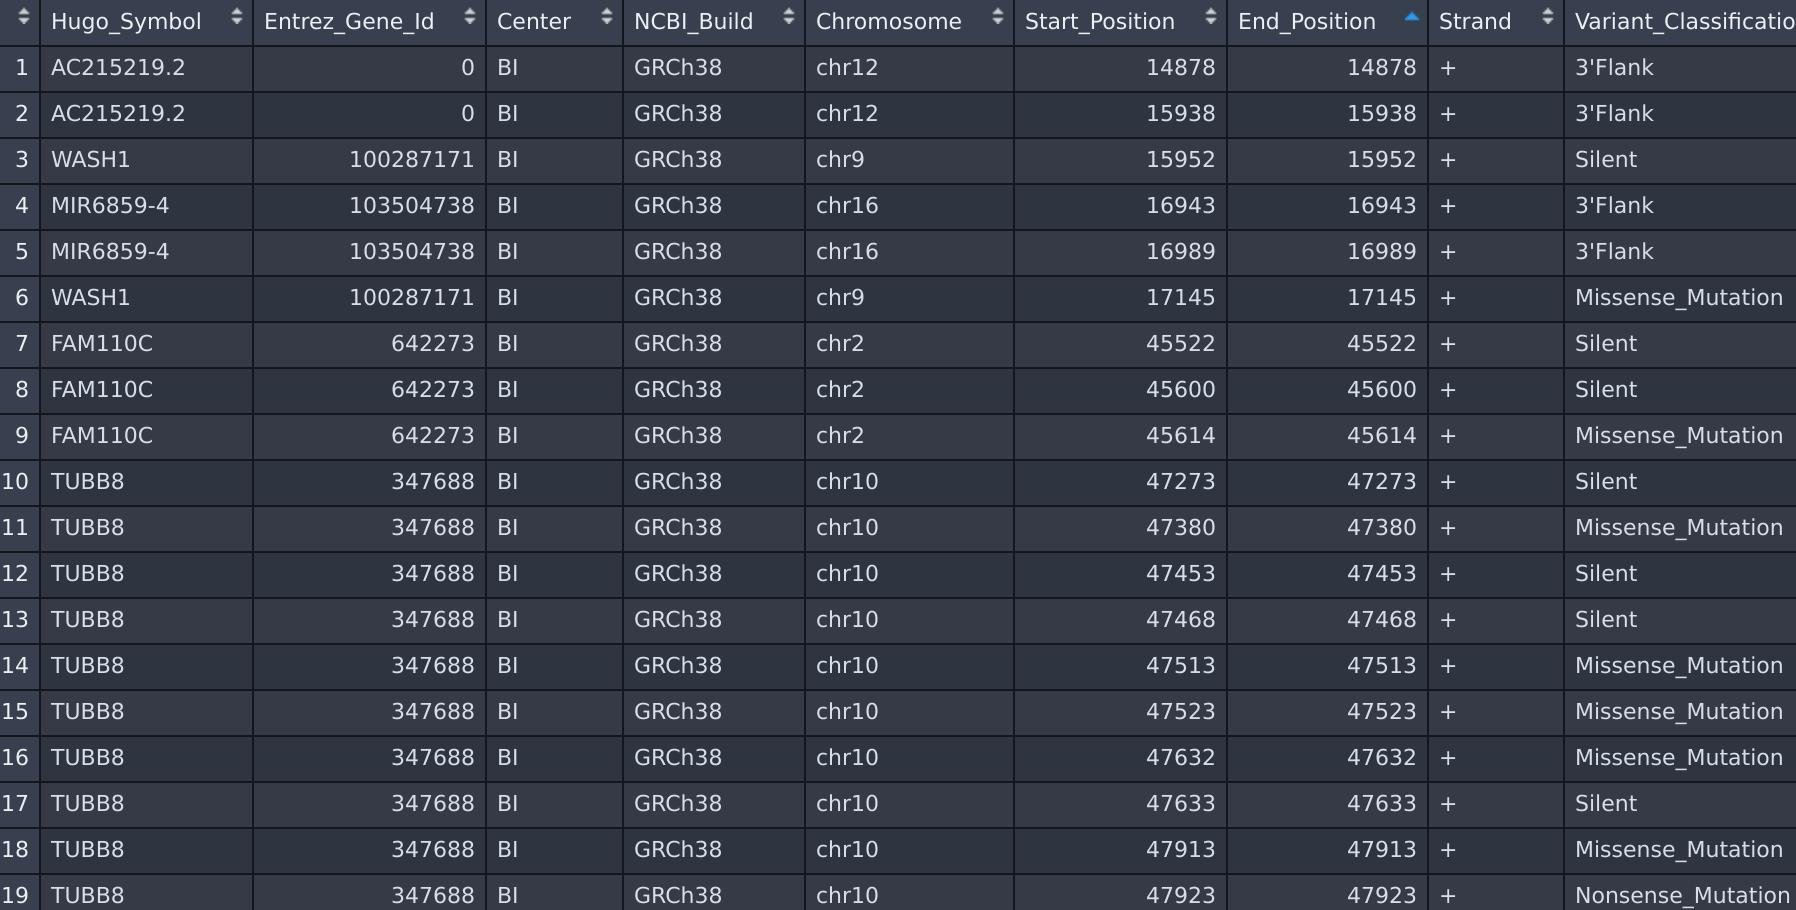
\includegraphics[scale = 0.15]{img/maf_r.jpg}
  \end{figure}
\end{frame}
\begin{frame}{MAF file II}
  \only<1>{
    \begin{block}{}
      We can plot information about the complete MAF file, using
      \textbf{Maftools R library} \cite{maftools}, such as:
      \begin{itemize}
        \item \textit{variant classification and type}
        \item \textit{single-nucleotide variant class}
        \item \textit{genes mutated more frequently}
      \end{itemize}
    \end{block}
    \begin{block}{Some passages of the marker paper can be found in these data}
      Past or present smoking associated with cytosine to adenine ($C>A$)
      nucleotide transversions as previously described both in individual genes
      and genome-wide \cite{luadmarker}.\\
      \textit{We will talk more about smokers}.
    \end{block}    
  }
  \only<2>{
    \begin{figure}
      \centering
      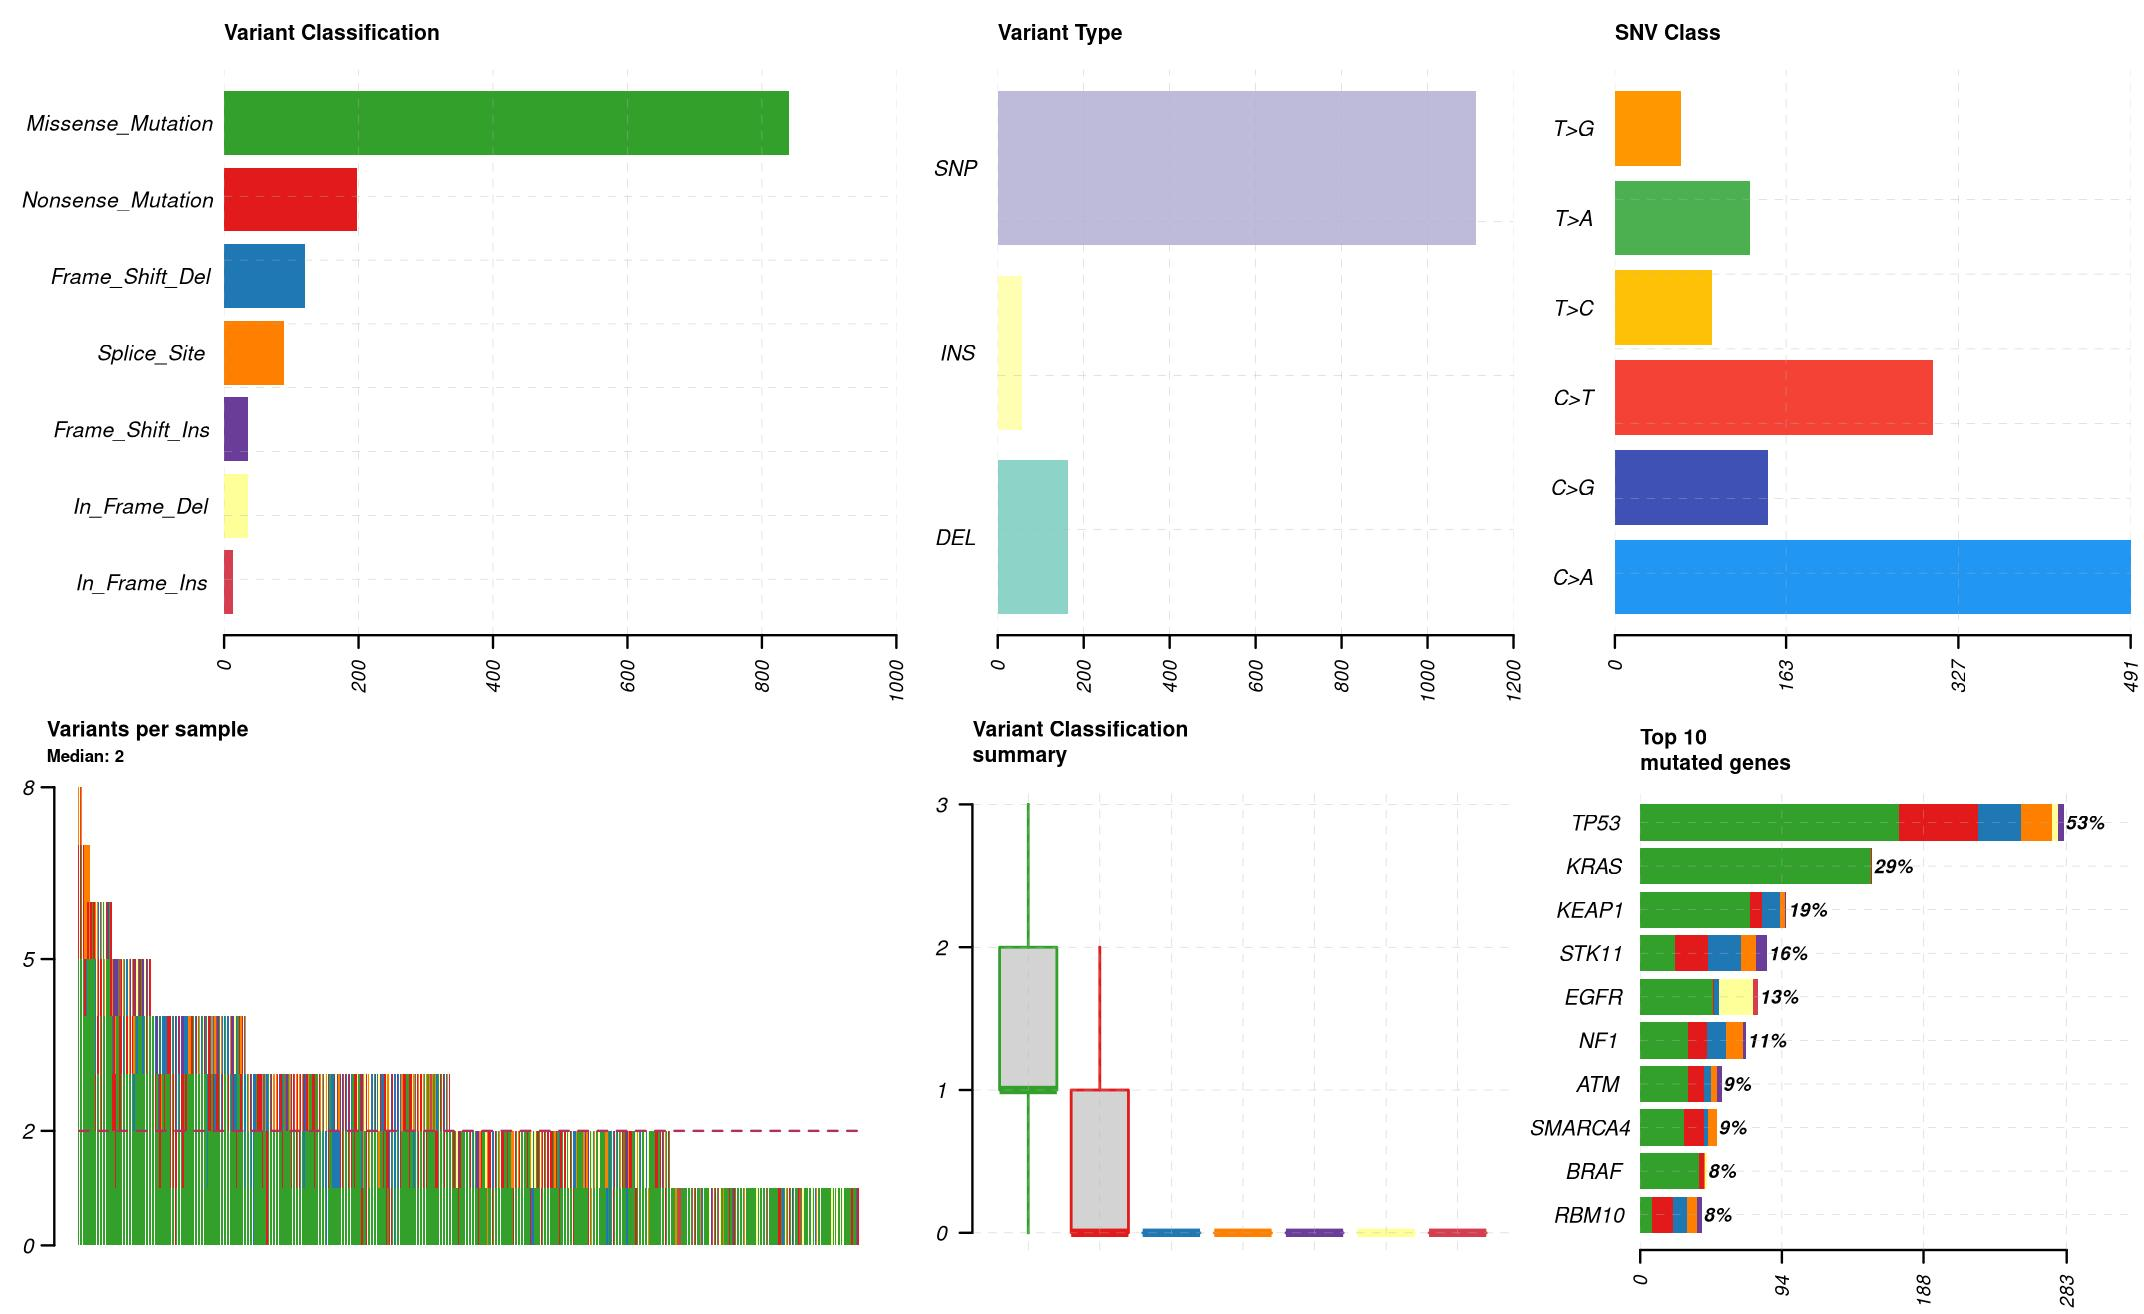
\includegraphics[scale = 0.135]{img/maf_reduced.jpg}
      \caption{\textbf{Maftools} analysis after the selection of the desired
        genes.} 
    \end{figure}
  }
\end{frame}
\begin{frame}{MAF file III}
  \only<1>{
    \begin{block}{MAF analysis with TRONCO library}
      By studying the file we have:
      \begin{itemize}
        \item 522 samples
        \item 38 genes
      \end{itemize}
      We decided to group each type of somatic mutation (such as
      \textit{missense mutations, nonsense mutations}, etc$\ldots$) into one
      type, simply noted as \textbf{Mutation}, therefore each gene is related to
      a single event.    
    \end{block}    
  }
  \only<2>{
    \begin{figure}
      \centering
      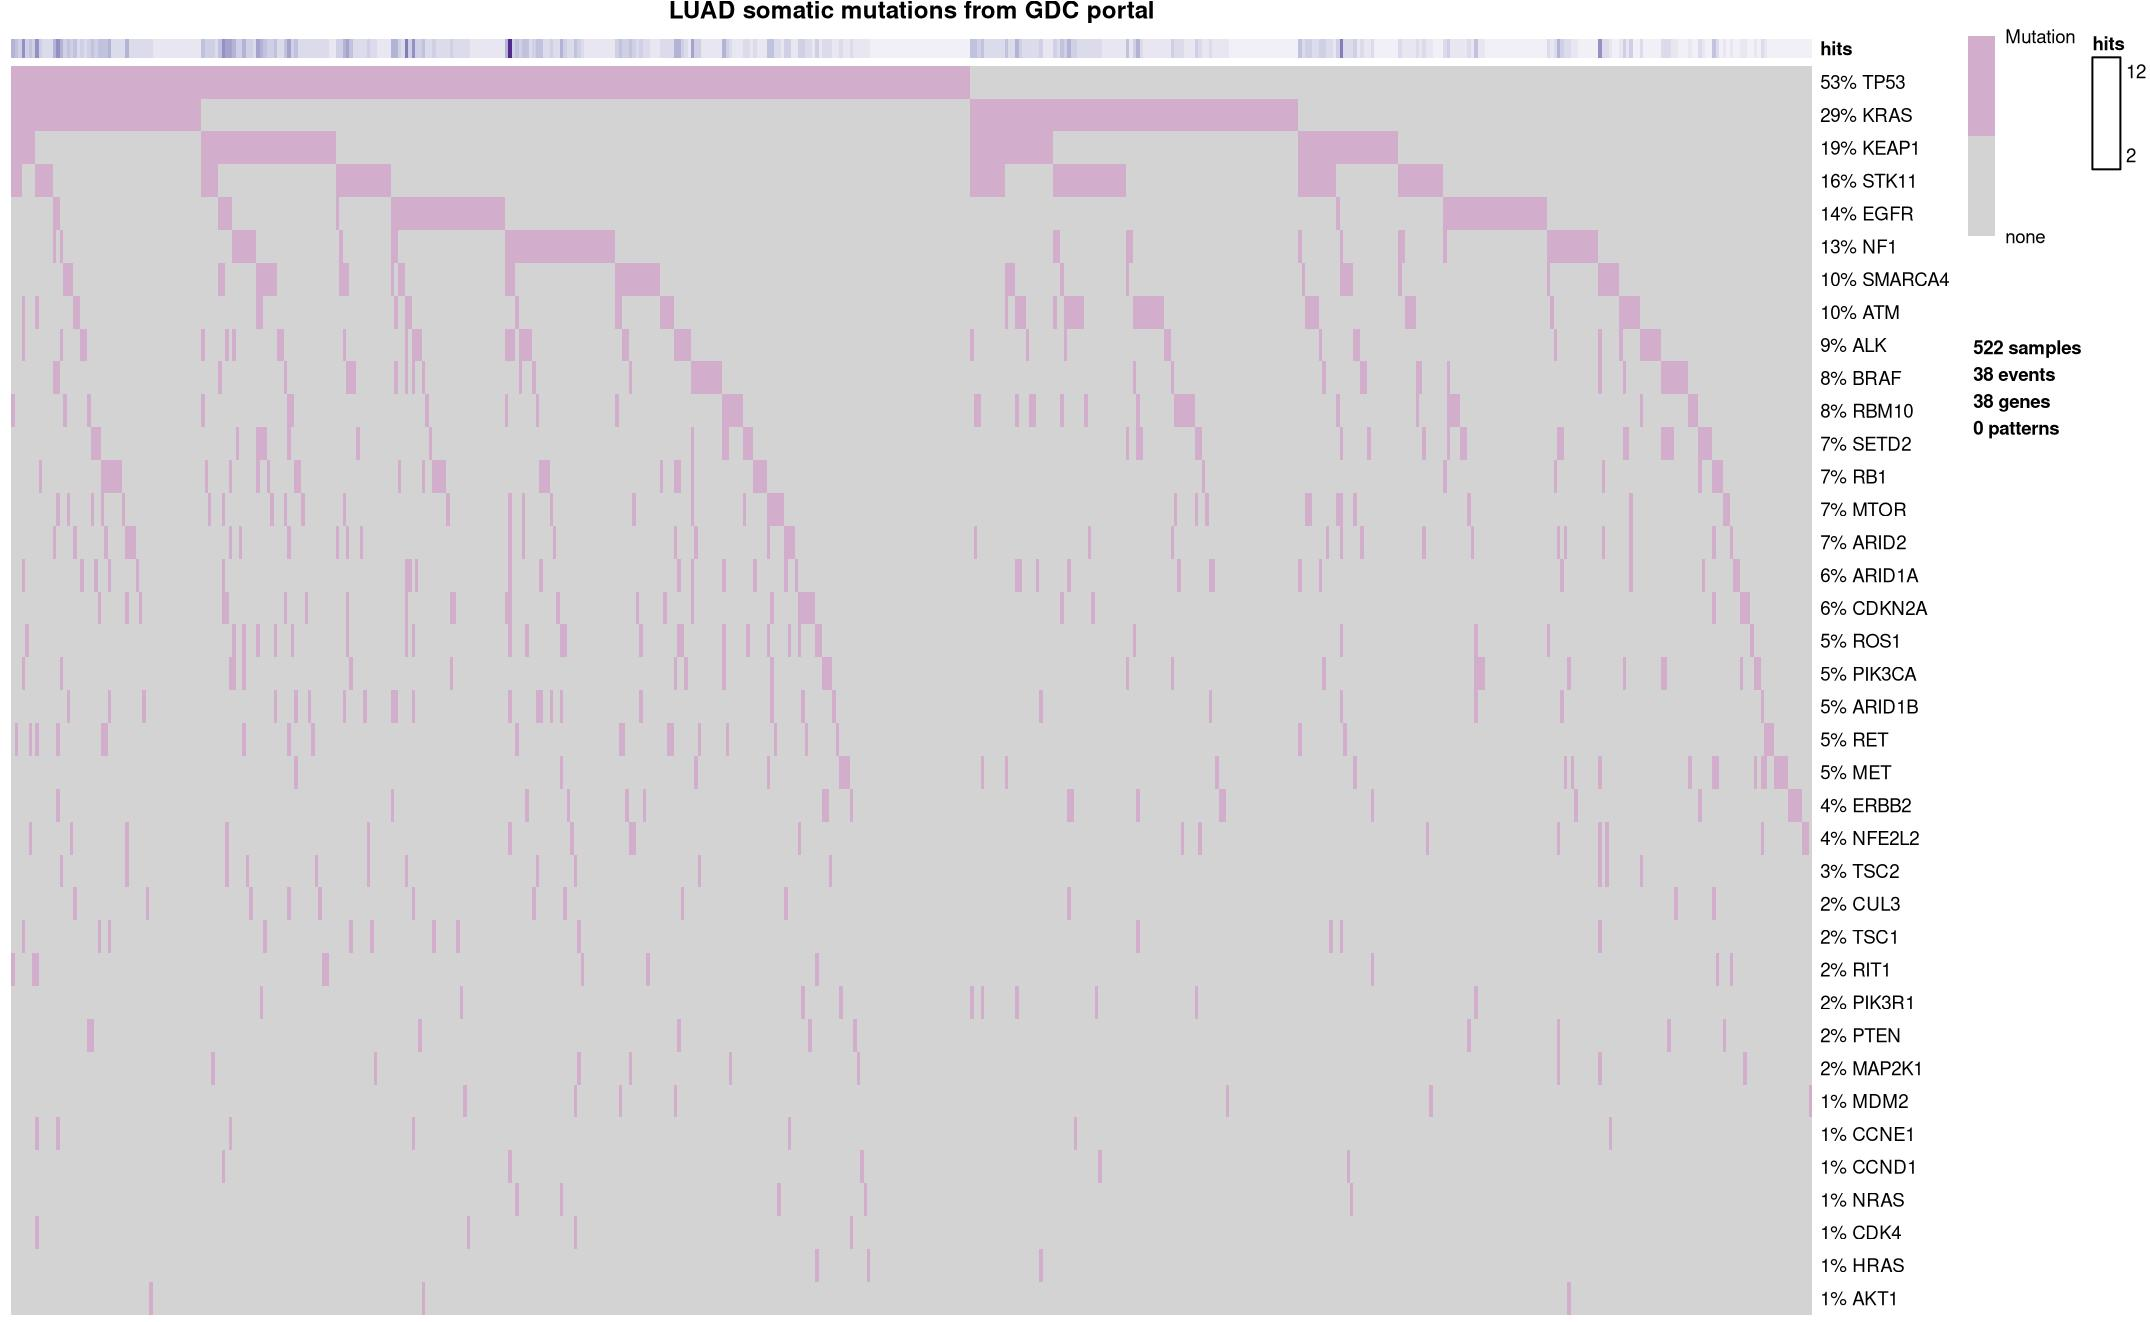
\includegraphics[scale = 0.135]{img/oncosom.jpg}
      \caption{Oncoprint of somatic mutations from MAF file.} 
    \end{figure}
  }
\end{frame}
\subsection{GISTIC}
\begin{frame}{GISTIC File I}
  \begin{block}{}
    Then we download data regarding \textit{CNAs}, annotated in the
    \textbf{GISTIC file}, where we have four mutation type \cite{cbioportal},
    each indicated with a value in the matrix: 
    \begin{enumerate}
      \item \textit{Homozygous loss (-2)}
      \item \textit{Heterozygous loss (-1)}
      \item \textit{Low-level gain (1)}
      \item \textit{High-level gain (2)}
    \end{enumerate}
    There is also 0 to indicate the absence of a mutation (\textit{Diploid})
  \end{block}
  \begin{figure}
    \centering
    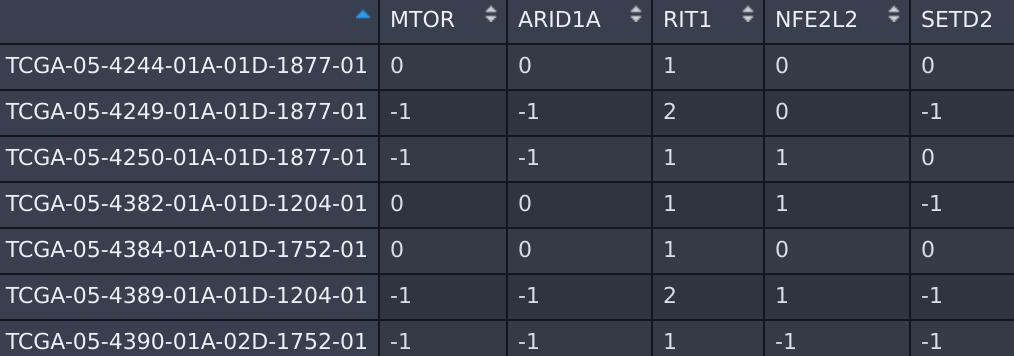
\includegraphics[scale = 0.22]{img/gistic_r.jpg}
  \end{figure}
\end{frame}
\begin{frame}{GISTIC File II}
  \only<1>{
    \begin{block}{}
      We decided to focus only on \textit{high-confidence scores}
      \cite{cbioportal}:  
      \begin{enumerate}
        \item \textit{Heterozygous loss (-1)}, as \textbf{Deletion}
        \item \textit{Low-level gain (1)}, as \textbf{Amplification}
      \end{enumerate}
    \end{block}
  }
  \only<2>{
    \begin{figure}
      \centering
      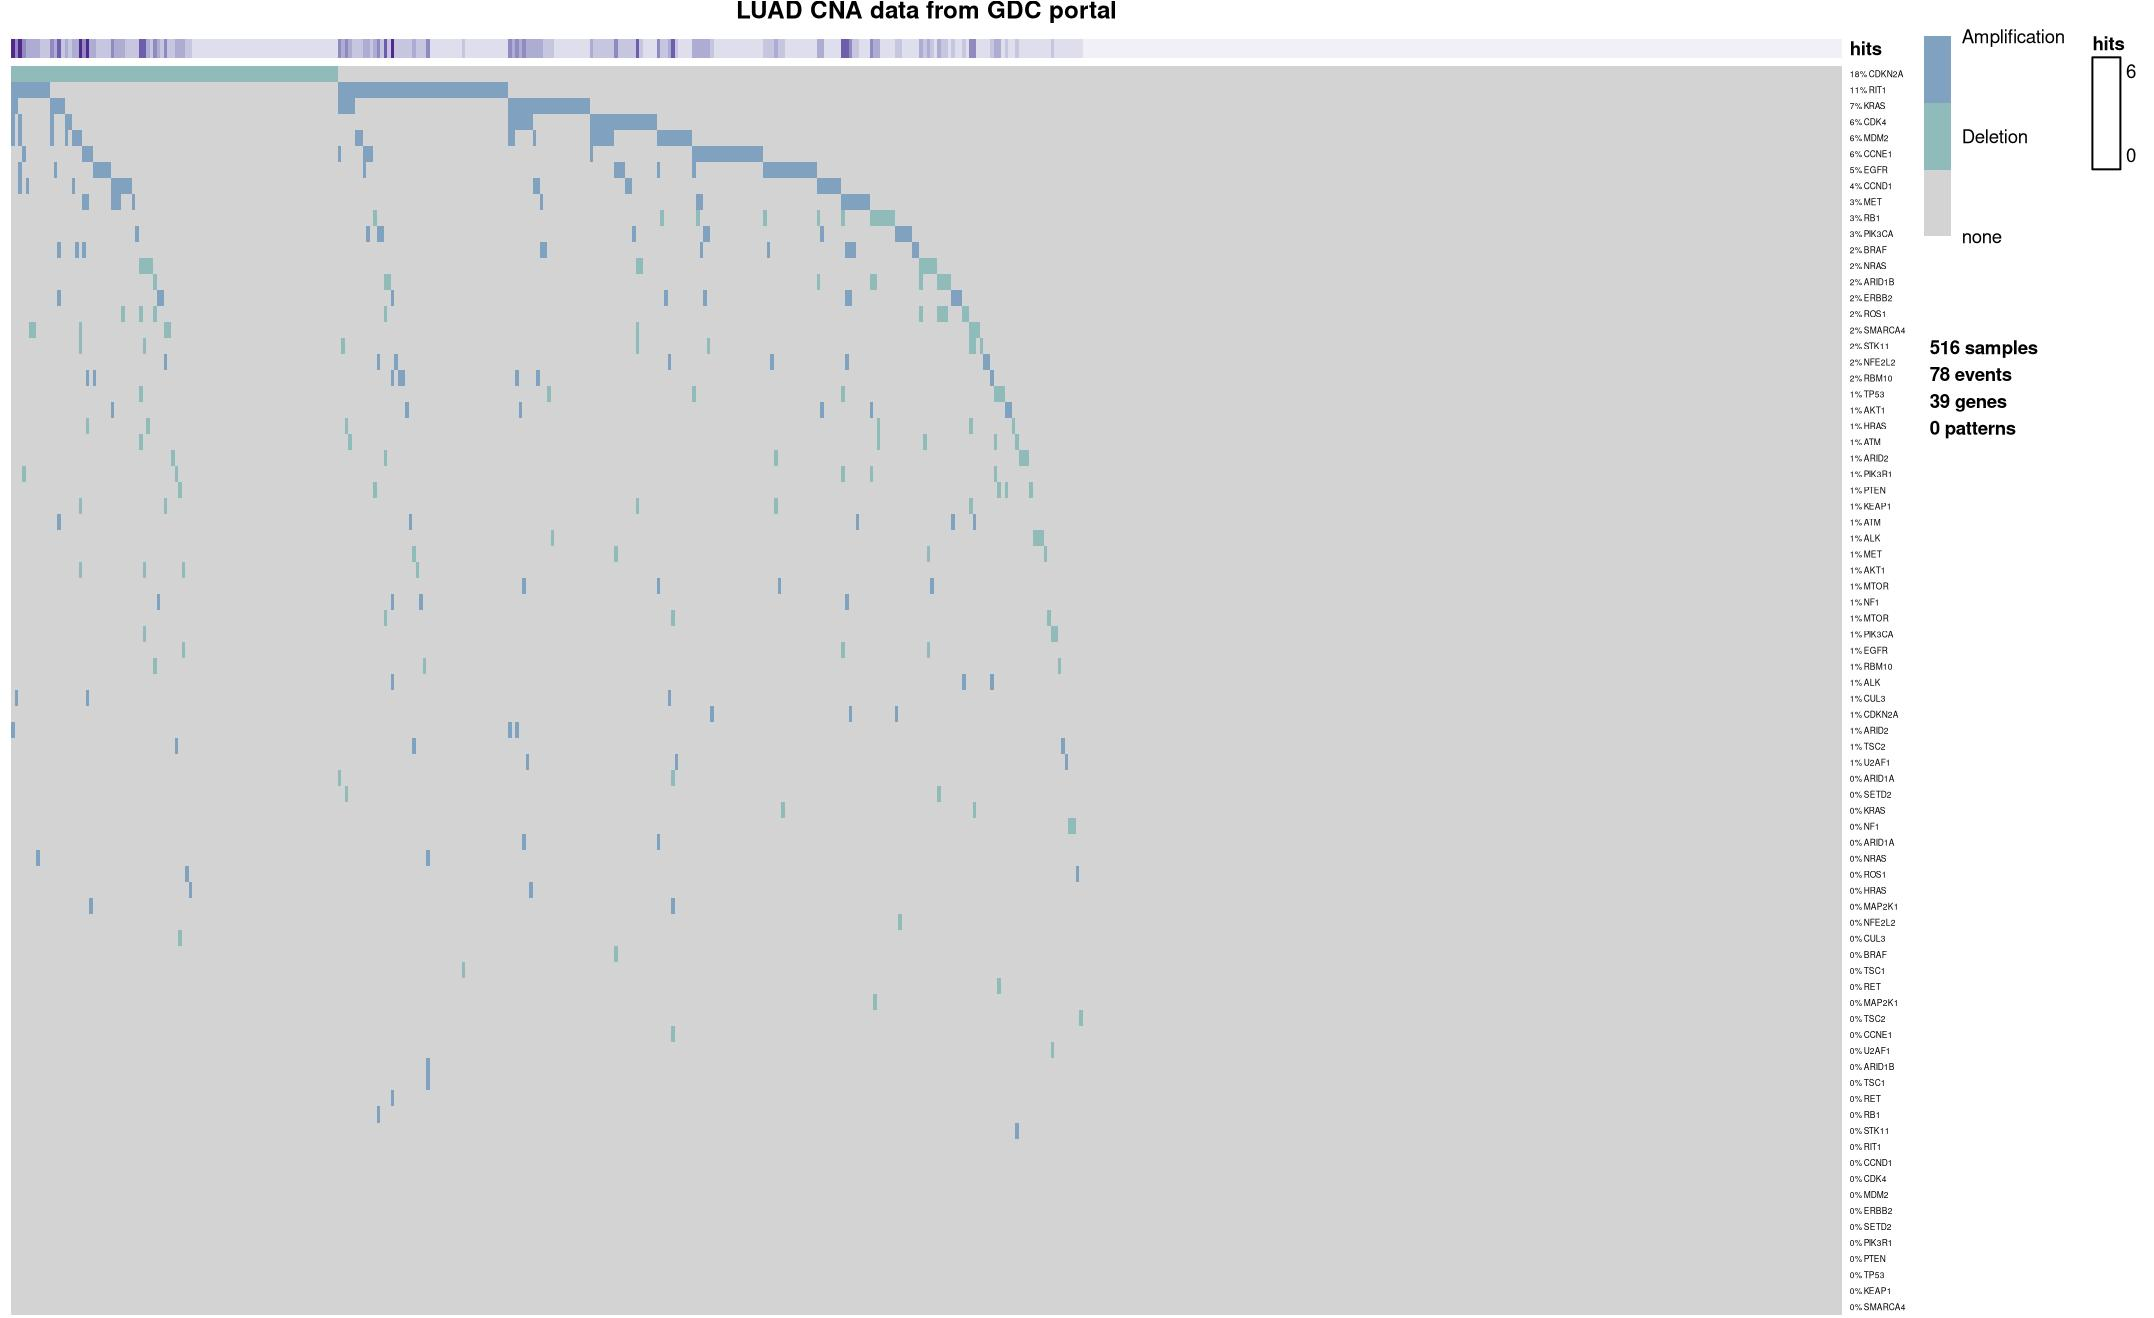
\includegraphics[scale = 0.135]{img/gisticonco.jpg}
      \caption{Oncoprint of selected CNAs from GISTIC file.} 
    \end{figure}
  }
\end{frame}
\subsection{Clinical}
\begin{frame}{Clinical data I}

  \begin{block}{}
    The next step was to download the clinical data, in order to have
    information, for most of the samples, regarding stages of tumor progression. 
  \end{block}
  
  \only<1>{
    \begin{block}{Clinical data information}
      In \textit{TCGA} we have clinical information on each sample such as:
      \begin{itemize}
        \item personal data (such as \textit{age, ethnicity} etc$\ldots$)
        \item temporal information about the tumor (such as \textit{date of
          initial diagnosis} etc$\ldots$)
        \item oncological data (such as \textbf{pathologic stage}
        etc$\ldots$)
        \item information on smoking 
      \end{itemize}
    \end{block}
  }
  \only<2>{
    \begin{figure}
      \centering
      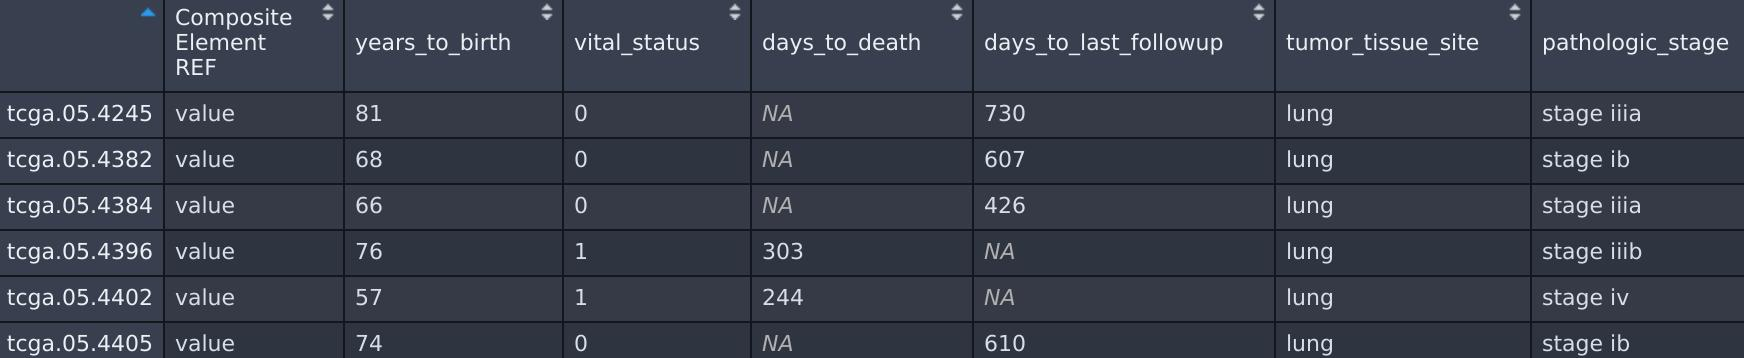
\includegraphics[scale = 0.19]{img/clinical_r.jpg}
    \end{figure}
  }
\end{frame}
\begin{frame}{Clinical data II}
  \begin{figure}
    \centering
    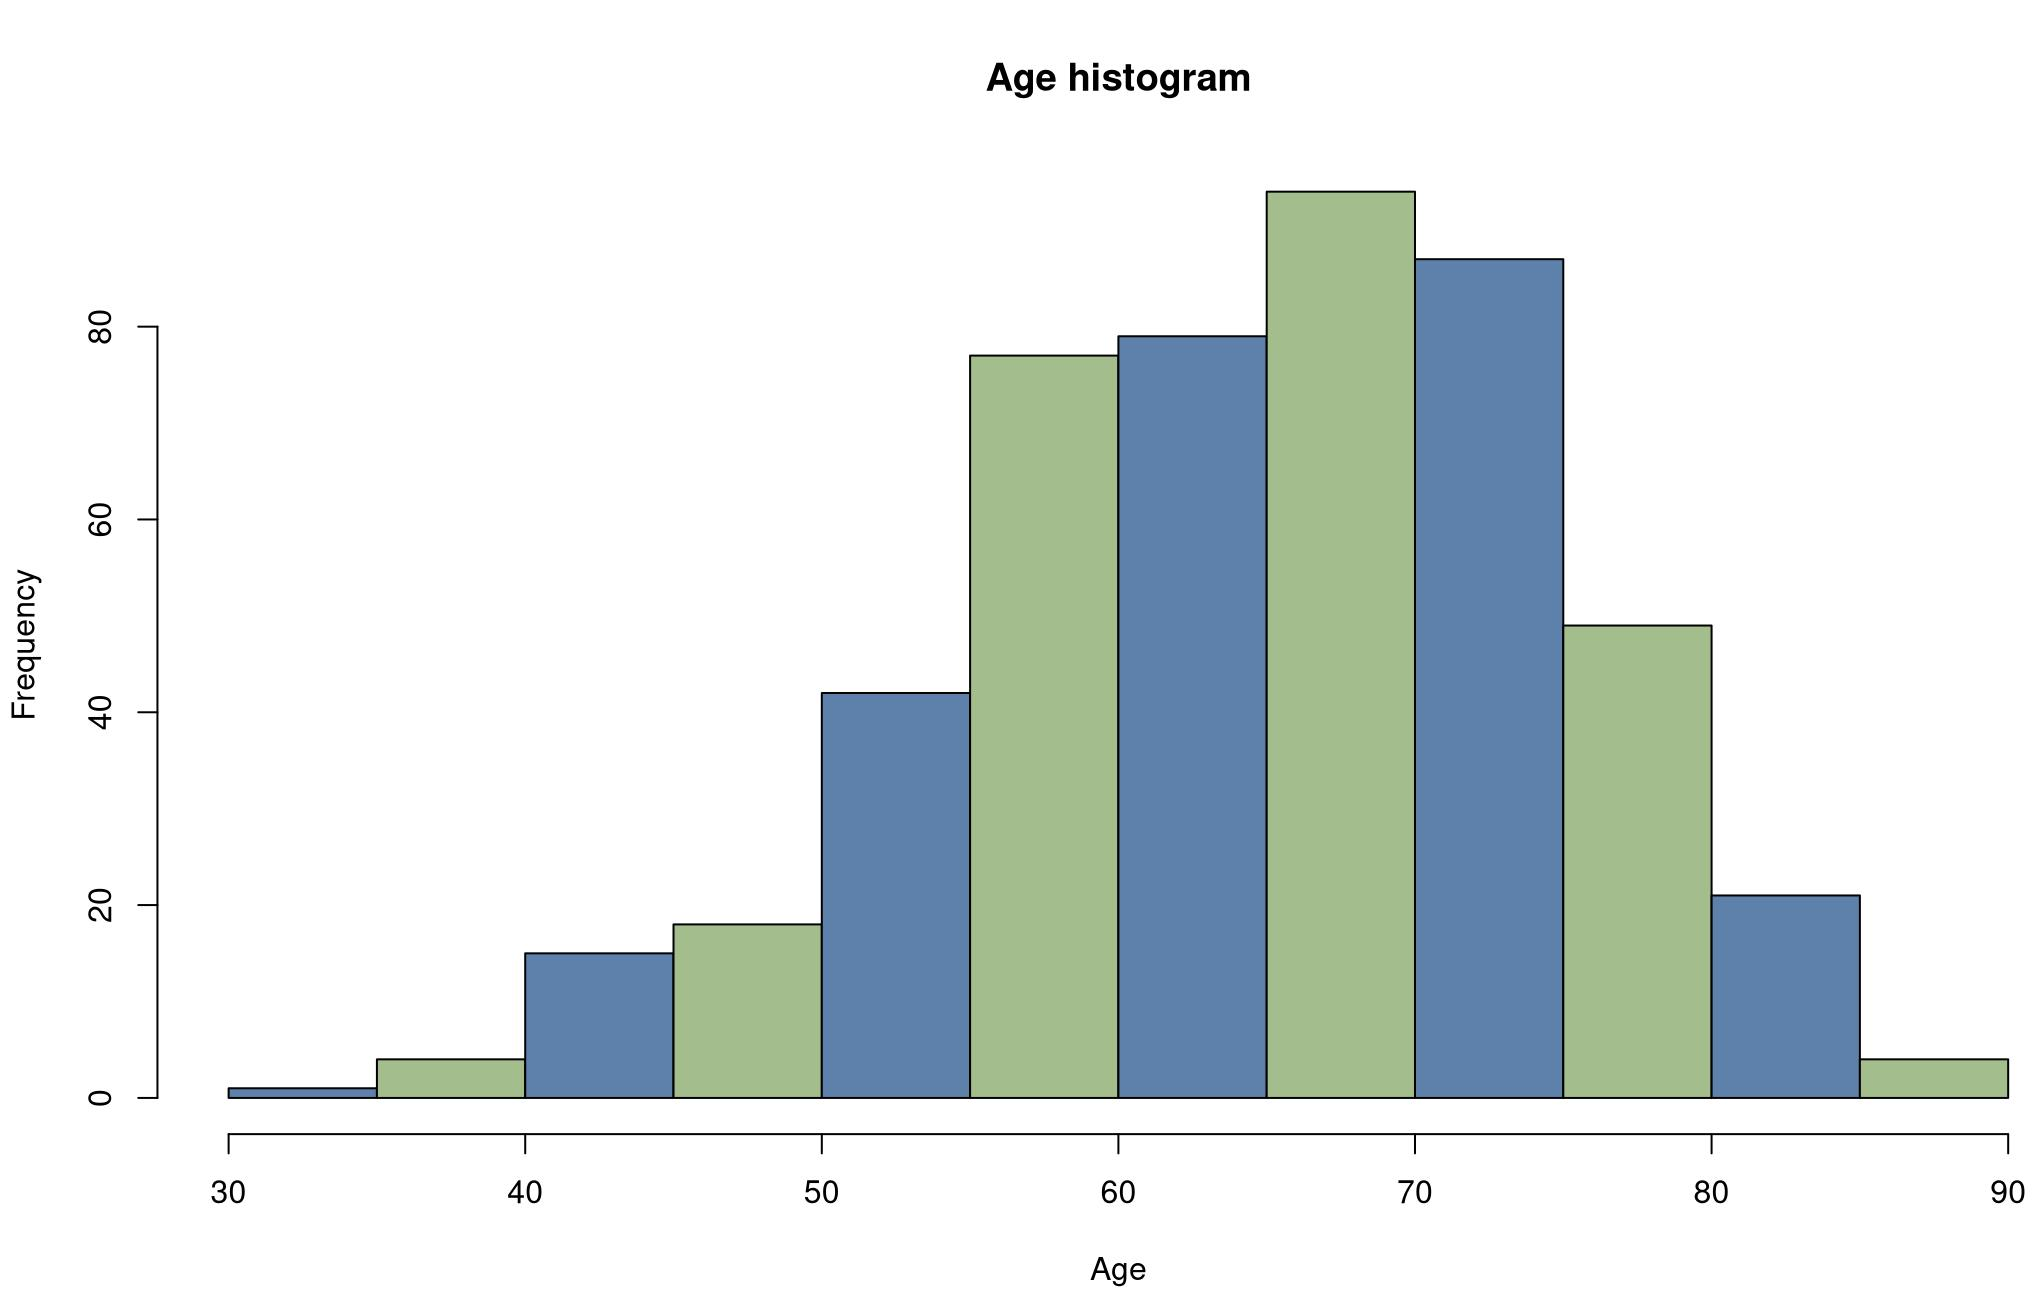
\includegraphics[scale = 0.082]{img/ages.jpg}
    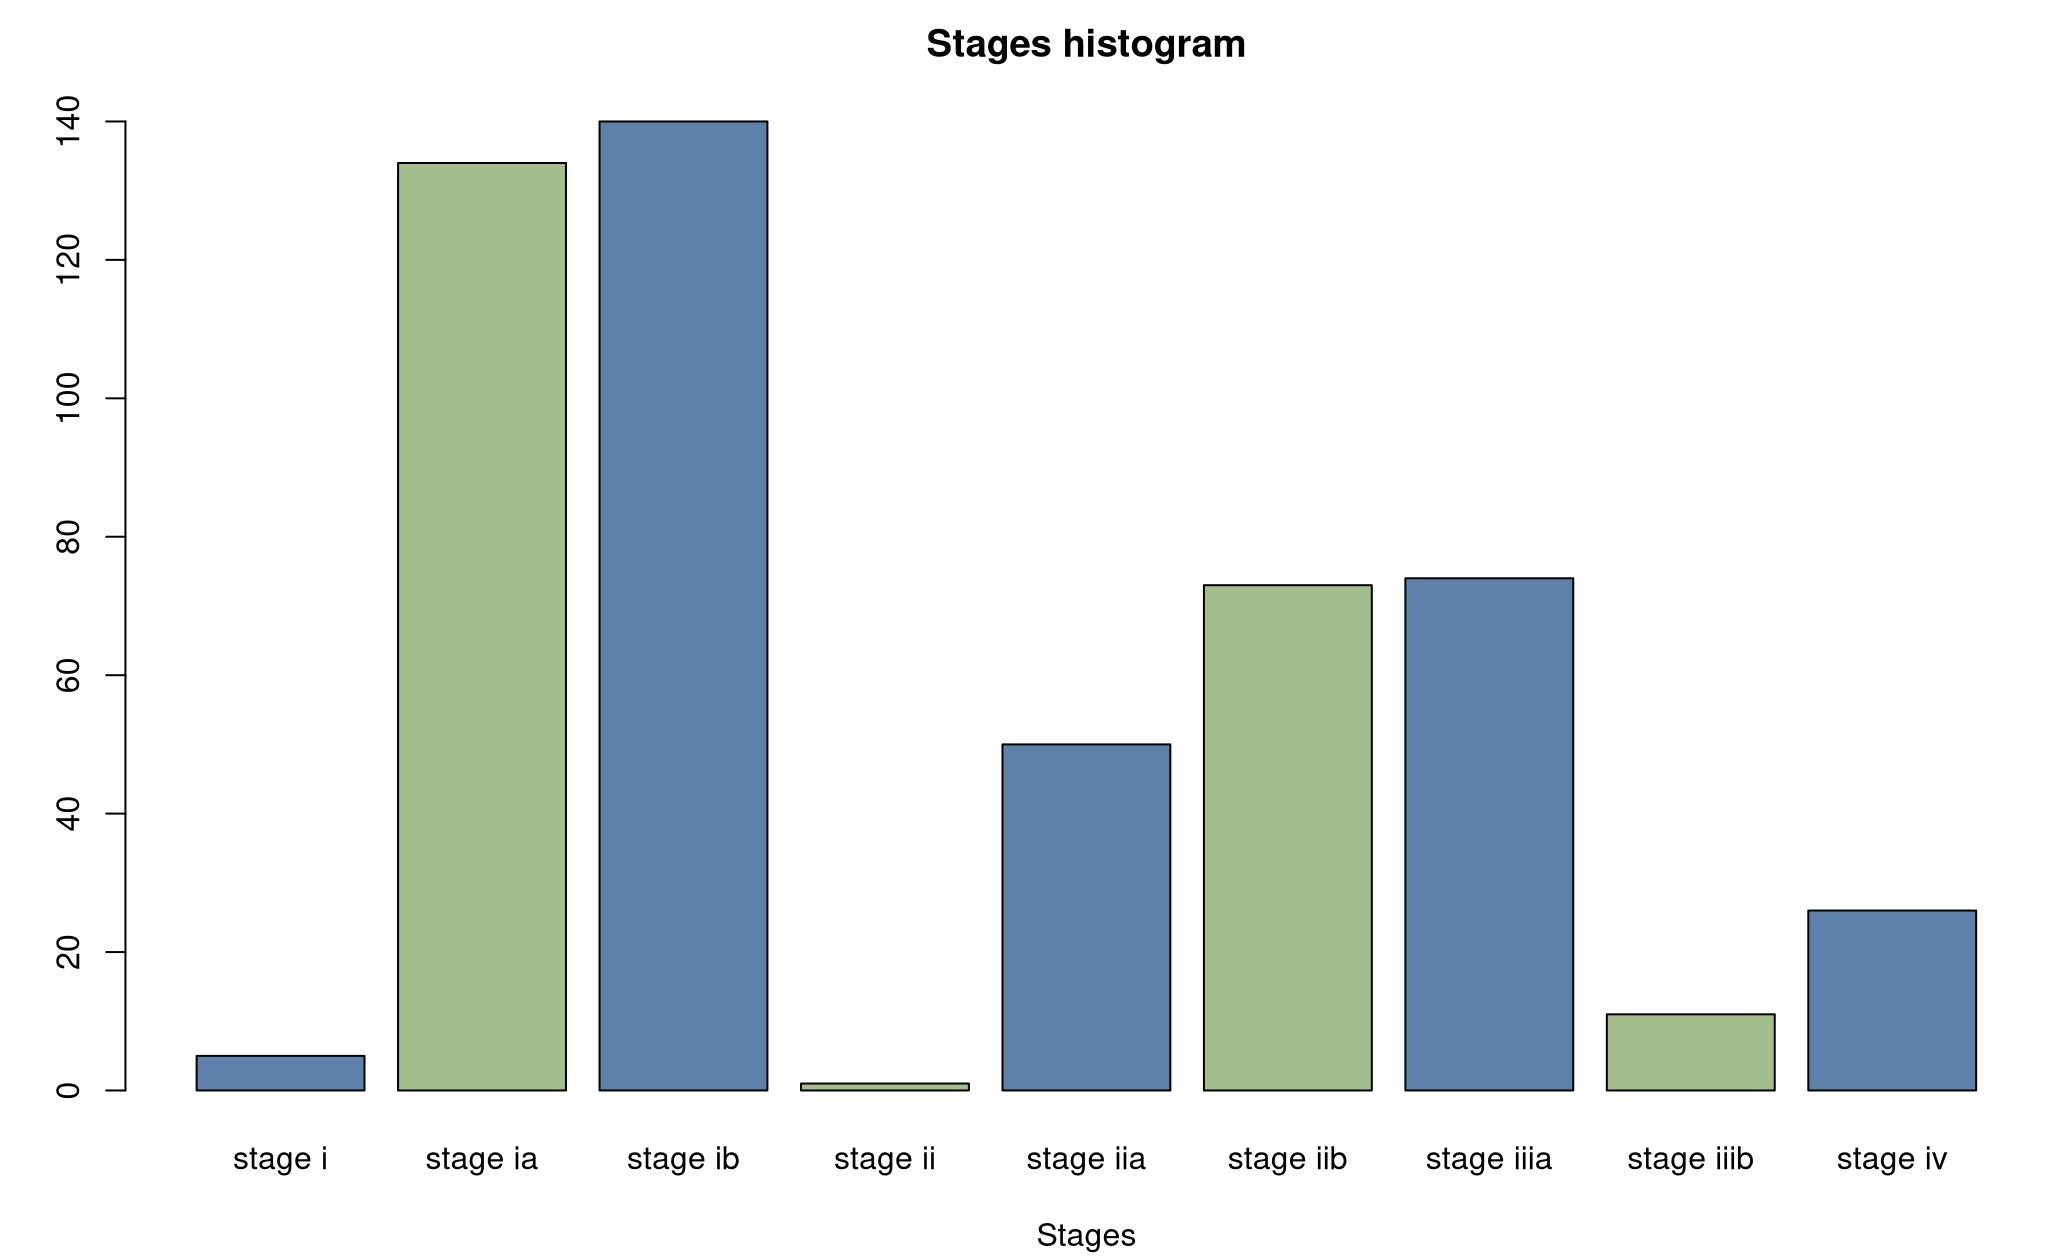
\includegraphics[scale = 0.082]{img/stages.jpg}
    \caption{Distribution of ages and tumor stages on samples.}
  \end{figure}
\end{frame}
\begin{frame}{Clinical data III}
  \begin{figure}
    \centering
    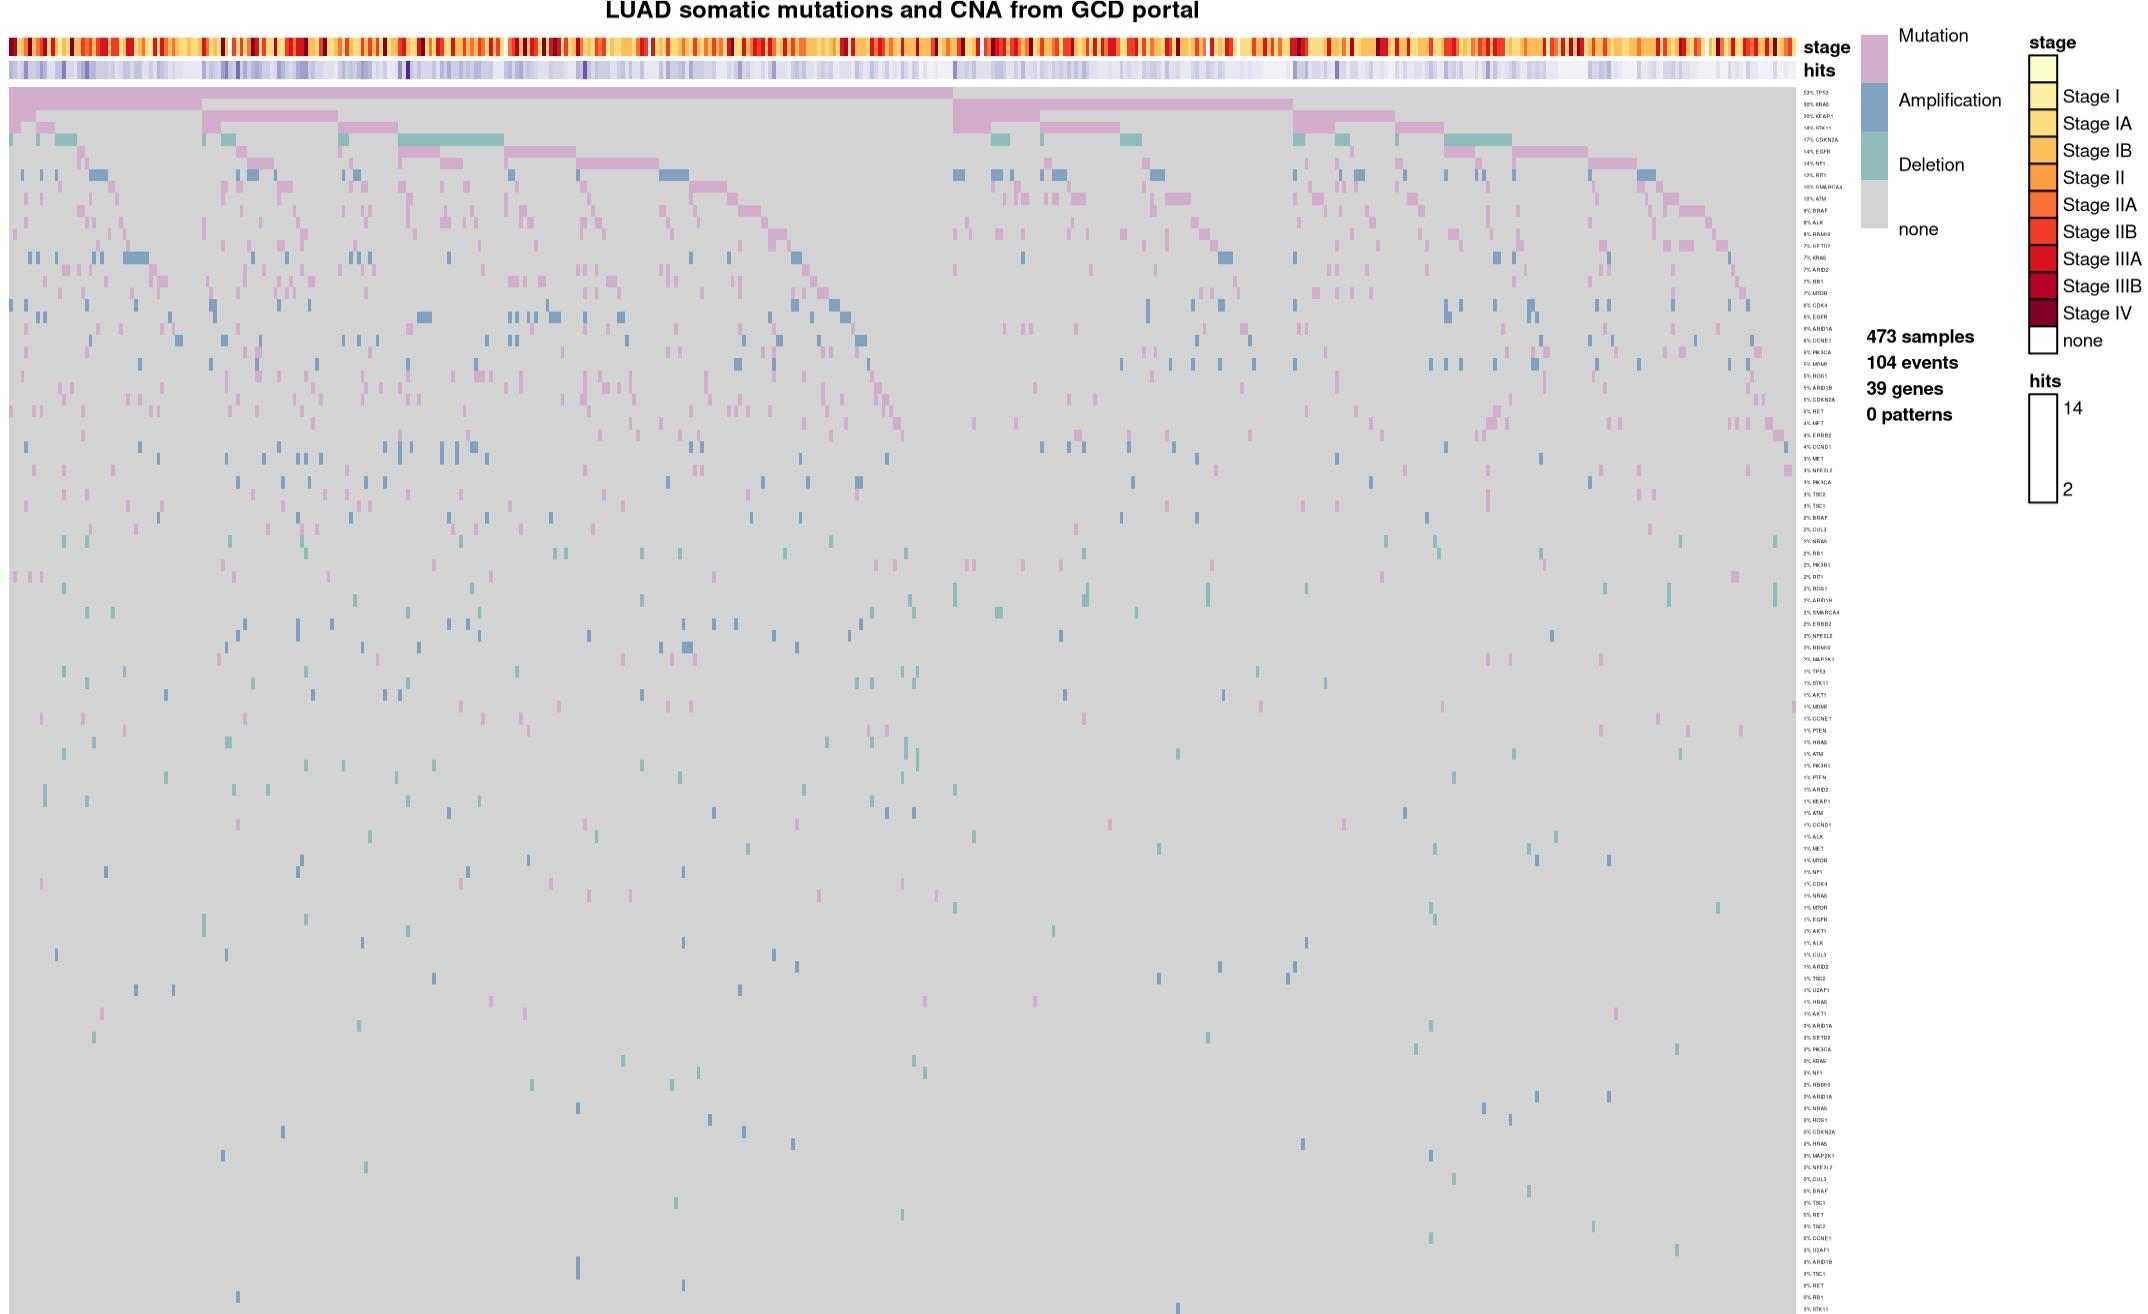
\includegraphics[scale = 0.135]{img/stageonco.jpg}
    \caption{Oncoprint of both somatic mutations and CNAs with tumor stages
      annotated.} 
  \end{figure}
\end{frame}
\begin{frame}{Smoke}
  \only<1>{
    \begin{block}{Smoking is one of the main causes of \textit{LUAD}}
      Speaking of lung adenocarcinoma, it is interesting to talk about
      smoking. The clinical data records, for some patients, the number of packs
      smoked per year, as well as the year they started smoking.  
    \end{block}
    \begin{figure}
      \centering
      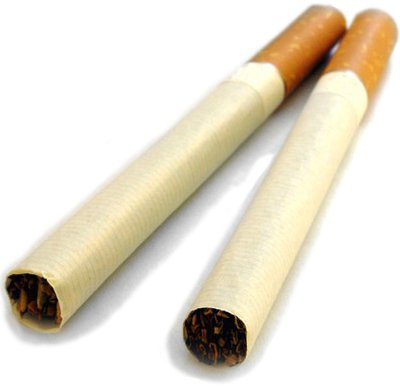
\includegraphics[scale = 0.145]{img/Cigarette.jpg}
    \end{figure}
  }
  \only<2>{
    \begin{figure}
      \centering
      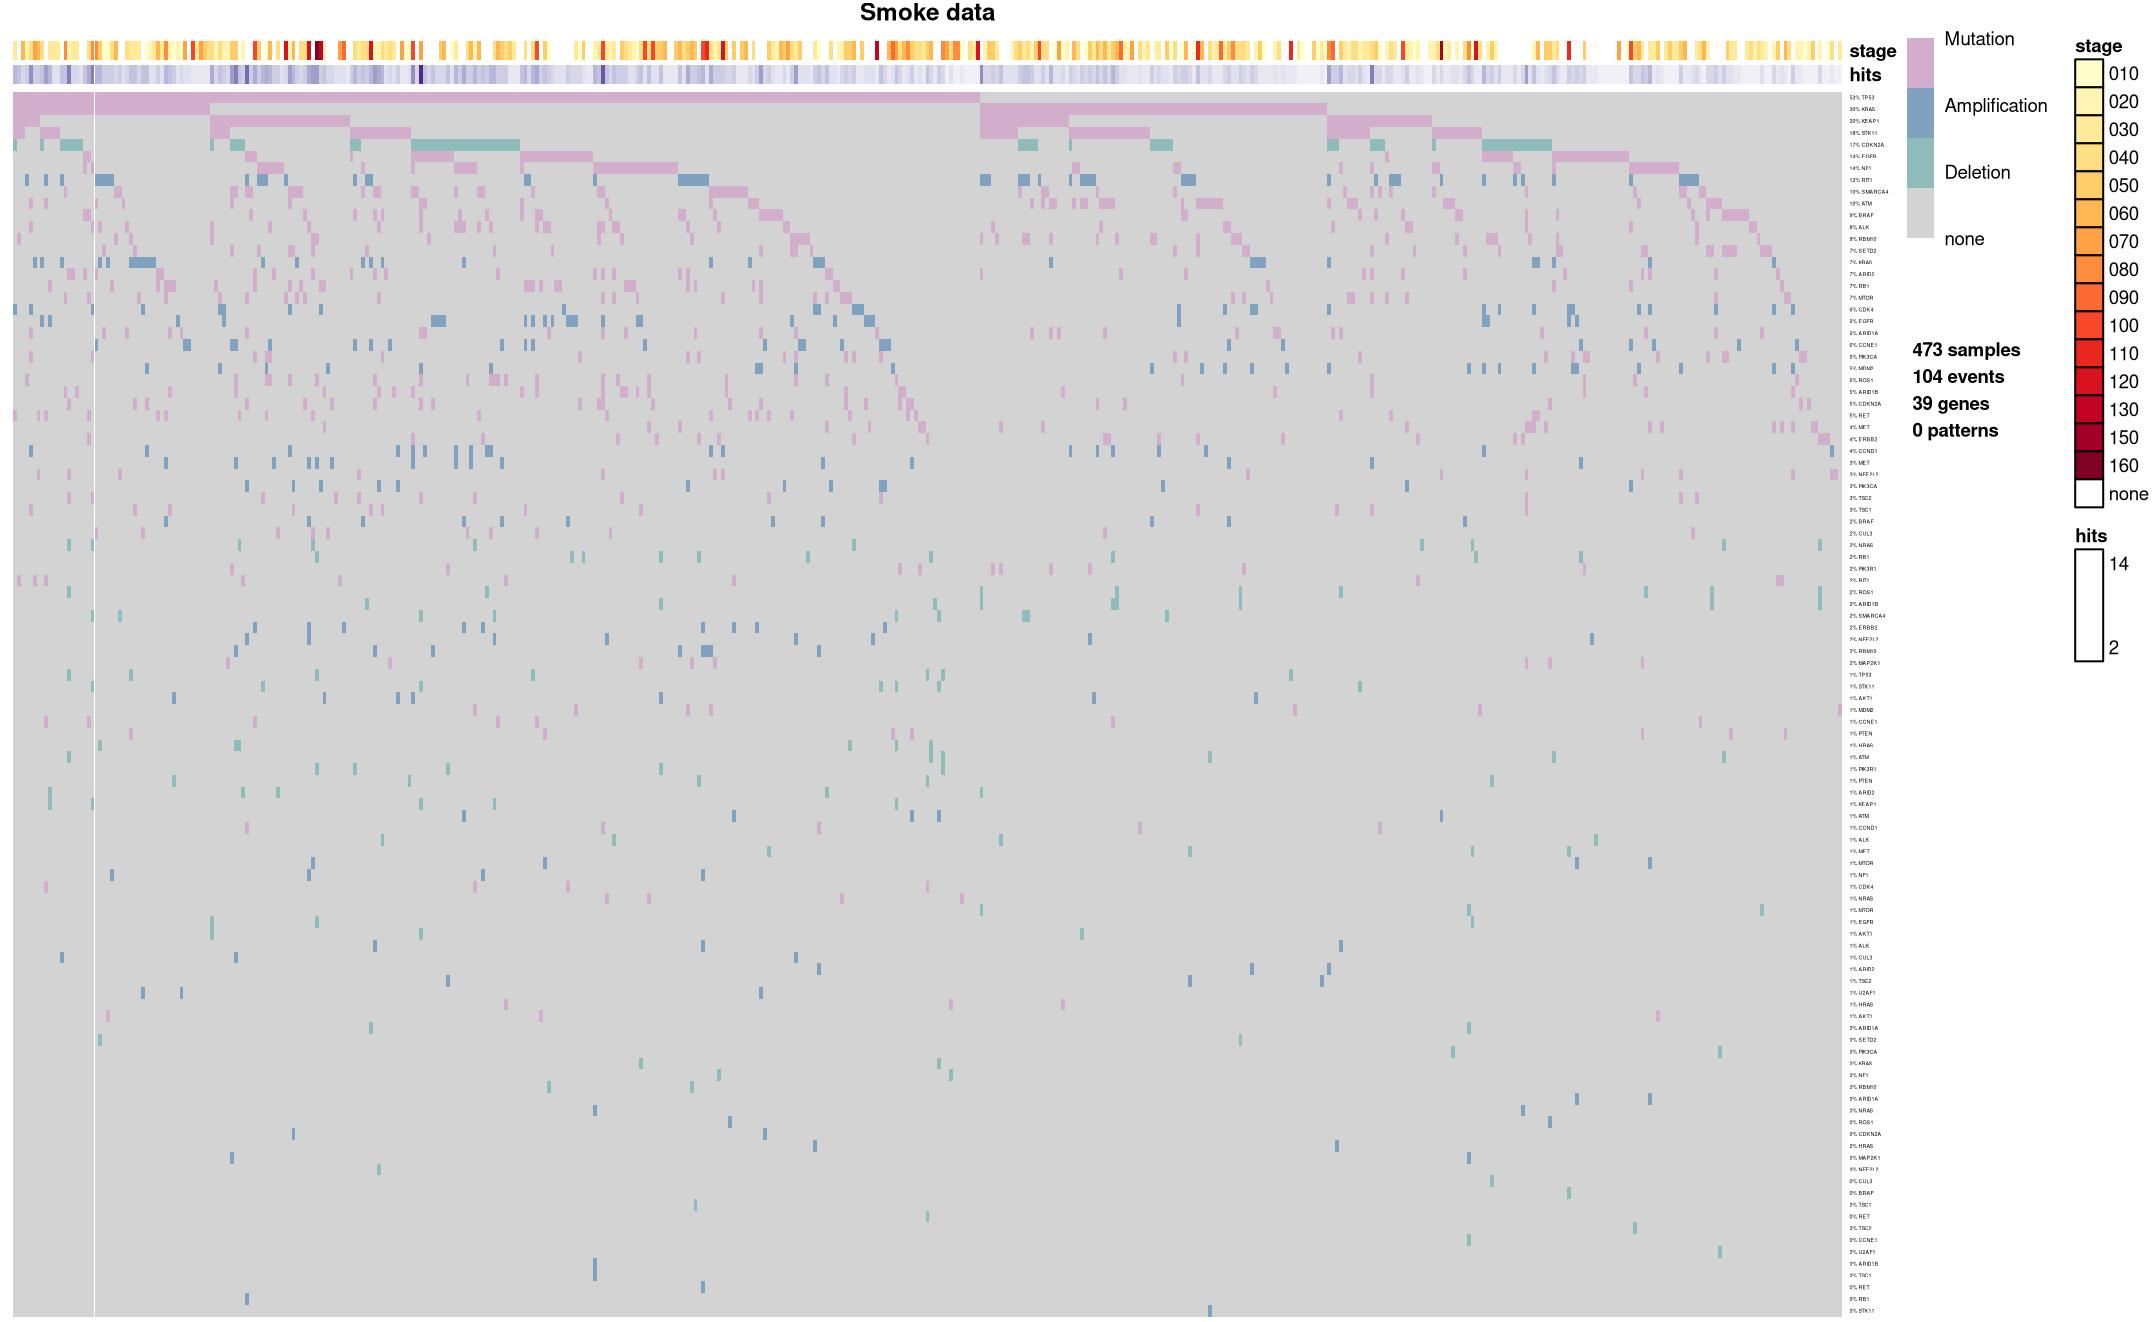
\includegraphics[scale = 0.135]{img/oncosmoke.jpg}
      \caption{A little ``hack'' to use \textit{oncoprint} function to plot the
        annotation of smoker in clinical data, using the number of packs smoked
        per year, grouped by tens, as ``stages''.} 
    \end{figure}
  }
\end{frame}
\subsection{Final Dataset}
\begin{frame}{Final TRONCO dataset for LUAD}
  \only<1>{
    \begin{block}{}
      As final preprocessing of the data we filter the events on the basis of a
      minimum frequency: $3\%$ \cite{dataclean}. 
    \end{block}
  }
  \only<2>{
    \begin{figure}
      \centering
      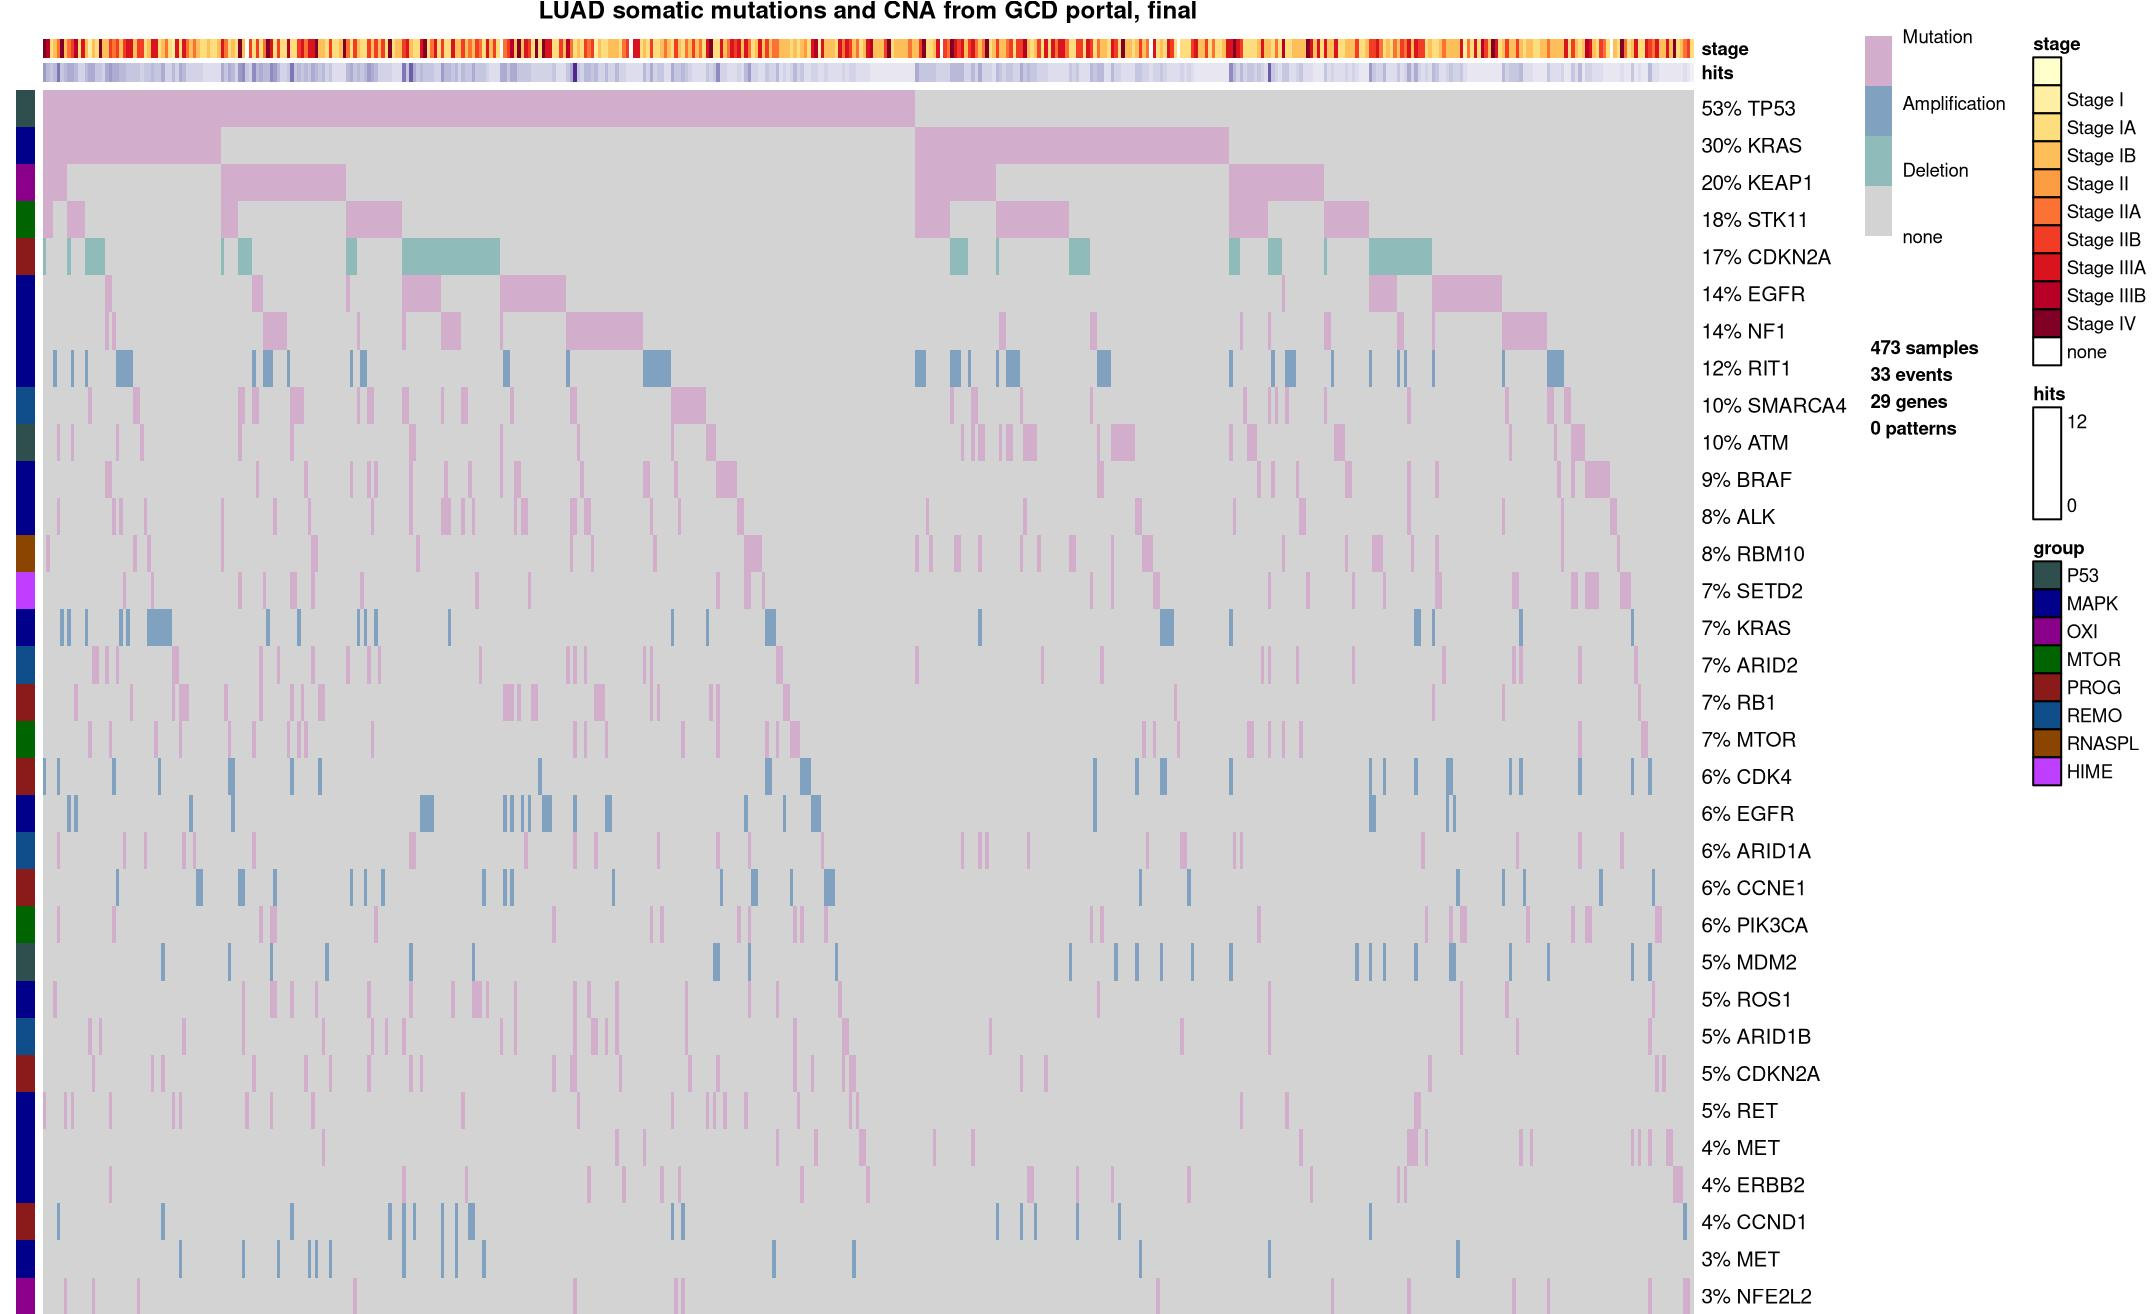
\includegraphics[scale = 0.135]{img/oncofinal.jpg}
      \caption{Oncoprint of complete dataset, after frequency selection, with
        stages and pathways annotated.} 
    \end{figure}
  }
\end{frame}
\section{Molecular Subtyping}
\begin{frame}{Subtyping I}
  \begin{block}{Marker paper subtyping}
    ``\textit{To coordinate naming of the transcriptional subtypes with the
      histopathological, anatomic and mutational classifications of lung
      adenocarcinoma, we propose an updated nomenclature: the \textbf{terminal
        respiratory unit} (\emph{TRU}, formerly bronchioid), the
      \textbf{proximal-inflammatory} (\emph{PI}, formerly squamoid), and the
      \textbf{proximal-proliferative} (\emph{PP}, formerly magnoid)
      transcriptional subtypes}'' \cite{luadmarker}. 
  \end{block}
  \pause
  \begin{block}{}
    Given these premises, we decided to study the three subtypes listed in the
    marker paper.\\
    \textit{Furthermore, for the sake of completeness, we have also decided to
      study the complete dataset without division into subtypes}. 
  \end{block}
\end{frame}
\begin{frame}{Subtyping II}
  \only<1>{
    \begin{block}{}
      In order to associate the respective subtype to a certain sample we again
      relied on TCGA, again through \textit{TCGAbiolinks}. 
    \end{block}
    \begin{figure}
      \centering
      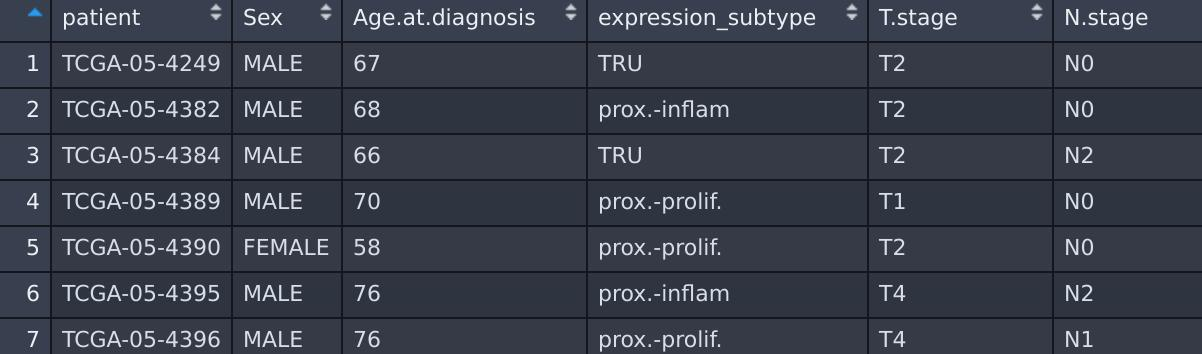
\includegraphics[scale = 0.23]{img/subtypes_r.jpg}
    \end{figure}
  }
\end{frame}
\begin{frame}{Subtyping III}
  \only<1>{
    \begin{figure}
      \centering
      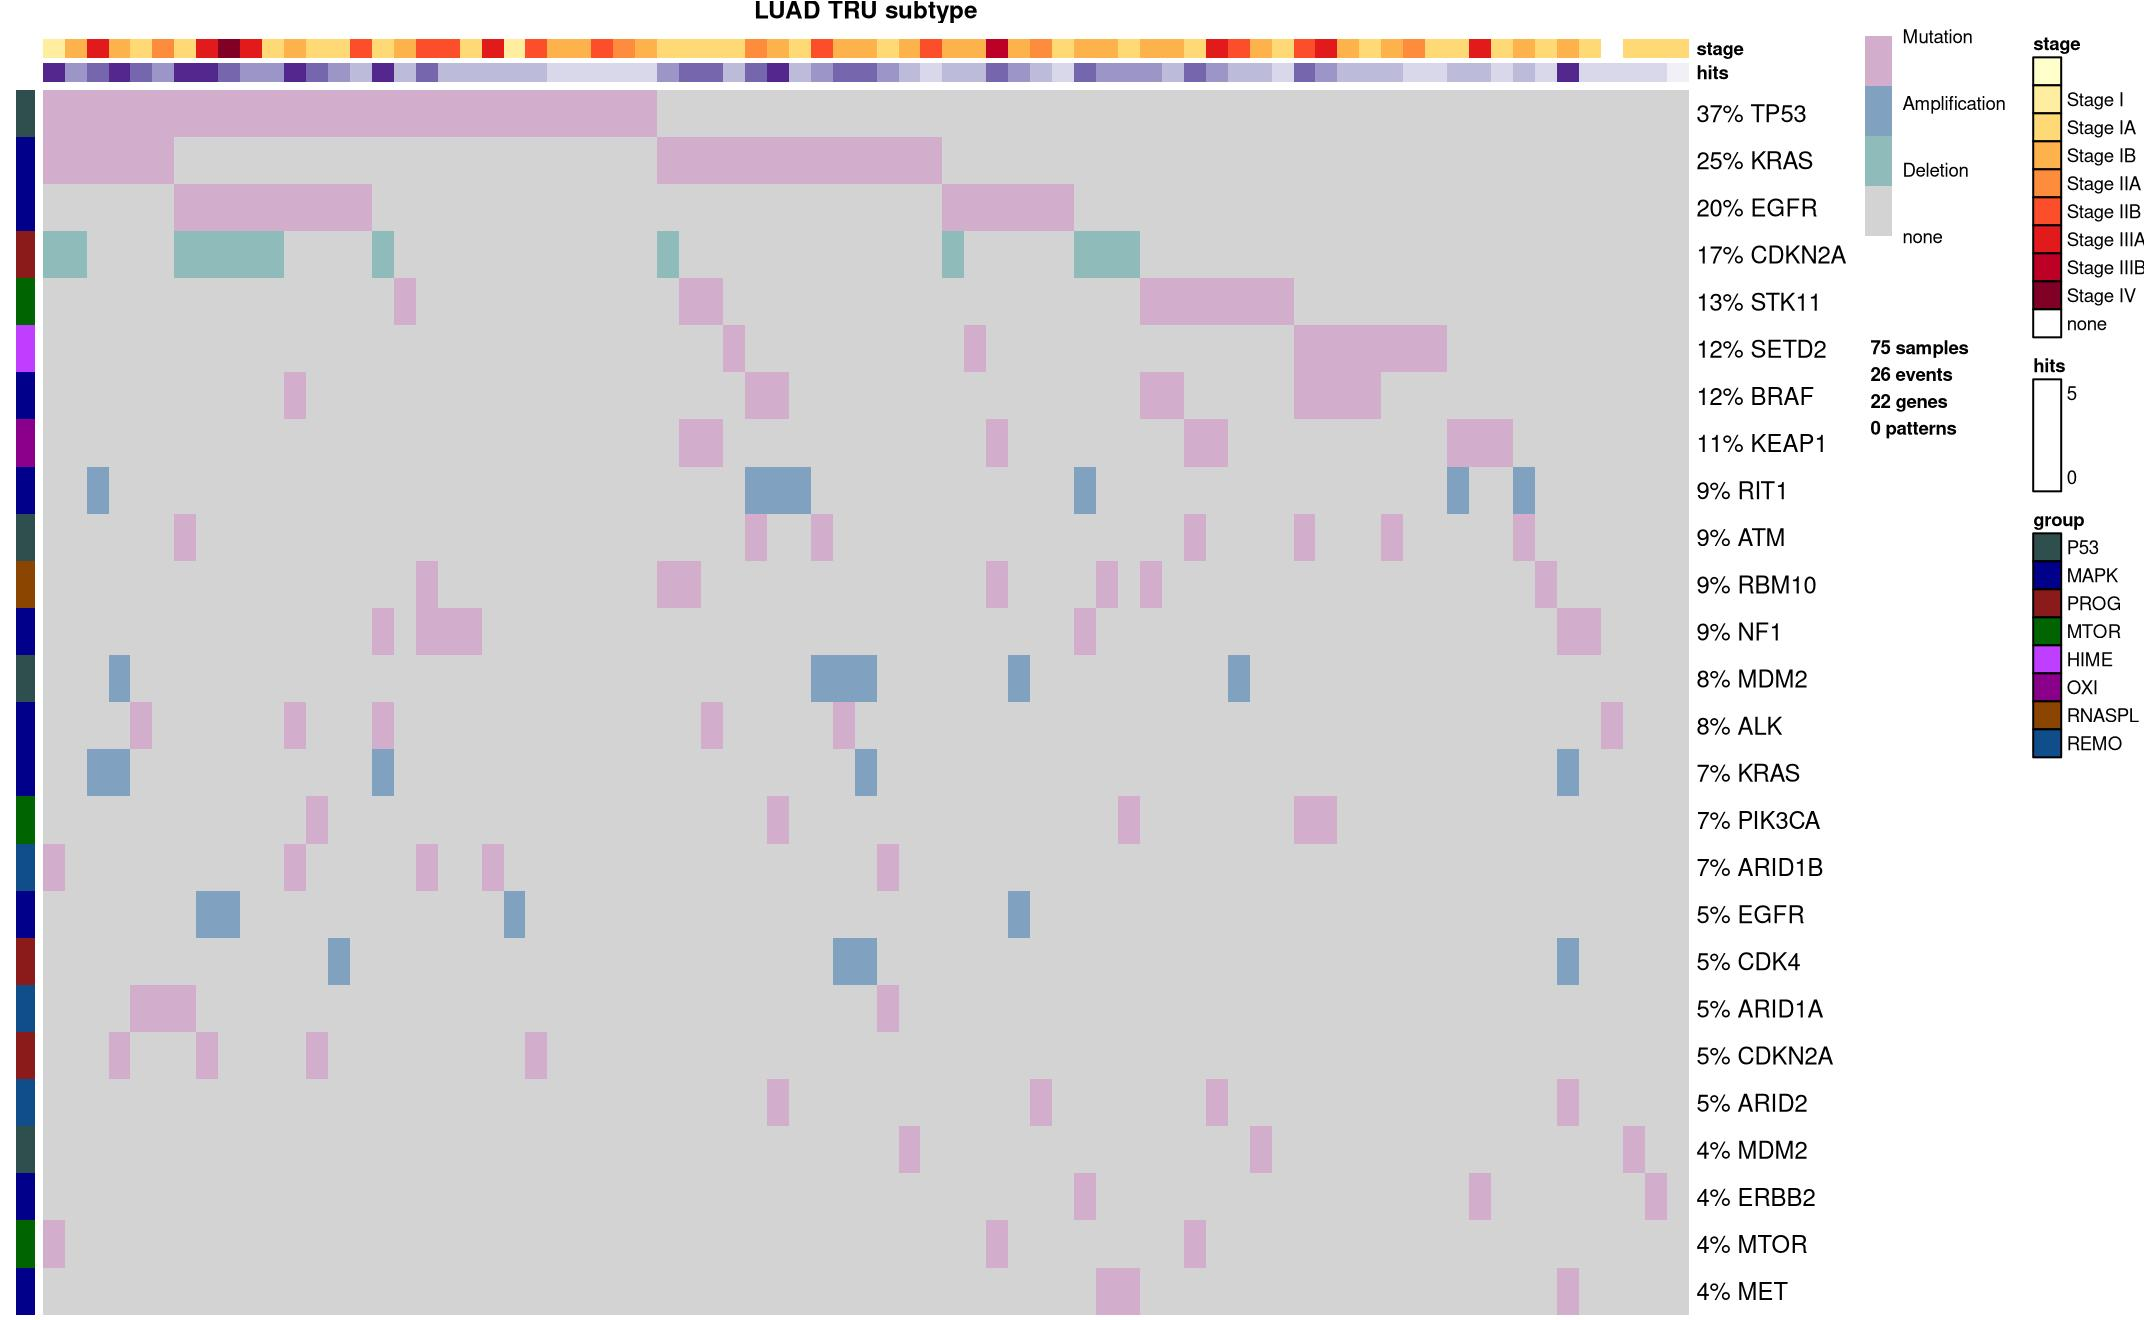
\includegraphics[scale = 0.135]{img/oncotru.jpg}
      \caption{Oncoprint of \textit{TRU} subtype, with stages and pathways
        annotated.}  
    \end{figure}
  }
  \only<2>{
    \begin{figure}
      \centering
      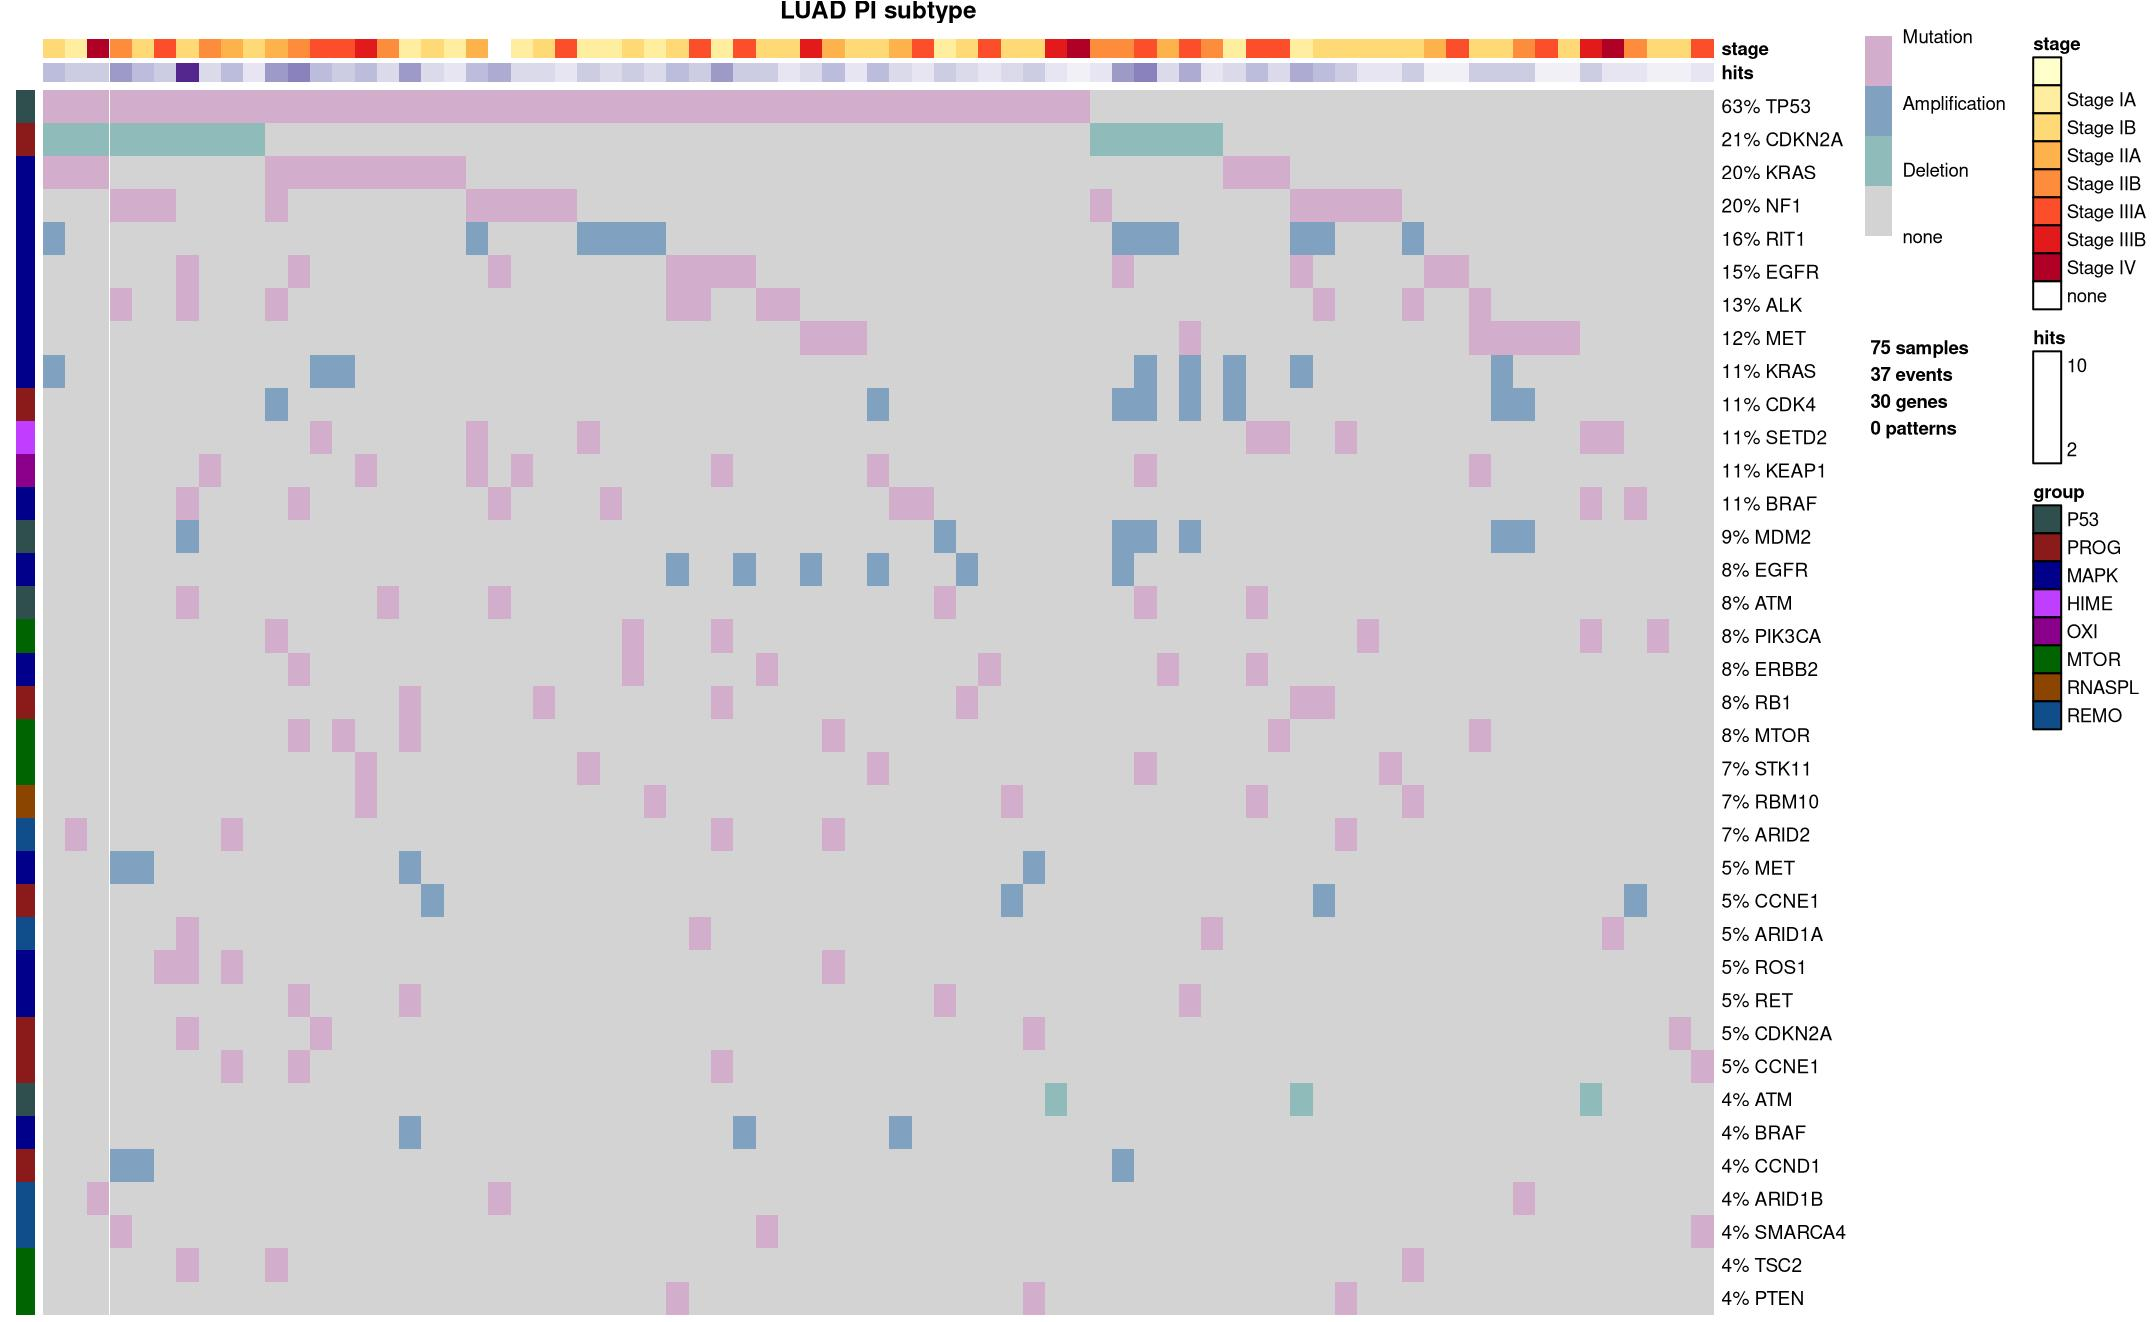
\includegraphics[scale = 0.135]{img/oncopi.jpg}
      \caption{Oncoprint of \textit{PI} subtype, with stages and pathways
        annotated.}  
    \end{figure}
  }
  \only<3>{
    \begin{figure}
      \centering
      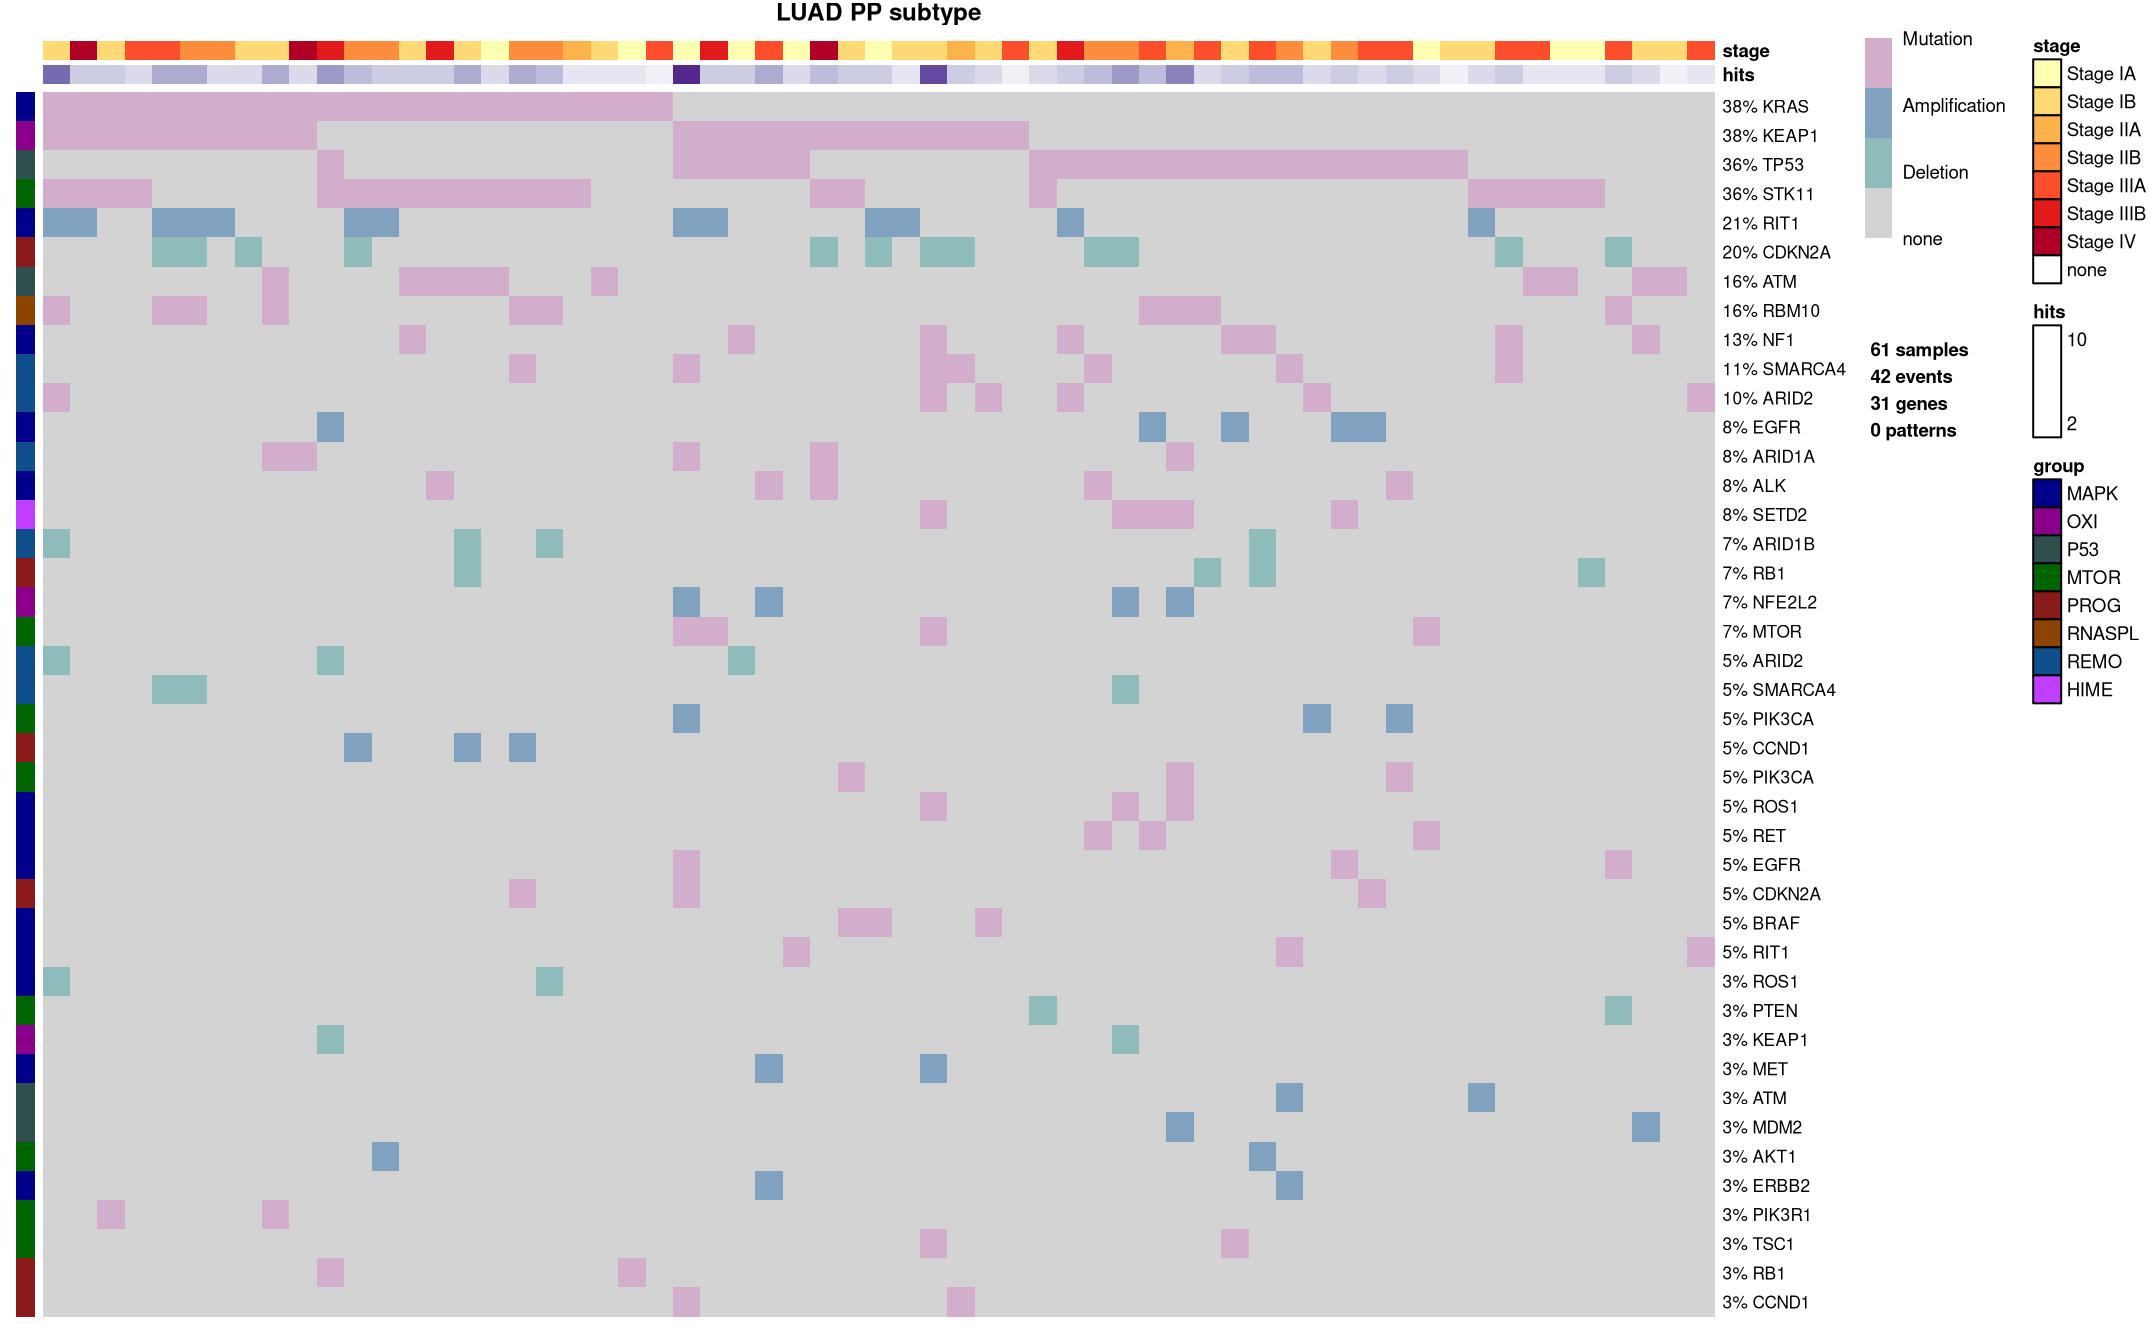
\includegraphics[scale = 0.135]{img/oncopp.jpg}
      \caption{Oncoprint of \textit{PP} subtype, with stages and pathways
        annotated.}  
    \end{figure}
  }
\end{frame}
\section{Group Exclusivity}
\subsection{Mutex}
\begin{frame}{Mutex I}
  \only<1>{
    \begin{block}{}
      As recommended by the authors of the PiCnIc pipeline, one of the main ways
      for the study of mutually exclusive groups is the use of a tool called
      \textbf{Mutex} \cite{dataclean}.
    \end{block}
    \begin{block}{}
      In any case, since the execution of this tool was very expensive, we
      used the results for LUAD already present in ``additional files'' of
      the paper. 
    \end{block}
    \begin{block}{}
      The file with all the results is imported through the \textit{TRONCO}
      utilities and then used to create hypotheses of mutually exclusive groups,
      making hypotheses with \textbf{OR}. 
    \end{block}
  }
  \only<2>{
    \begin{figure}
      \centering
      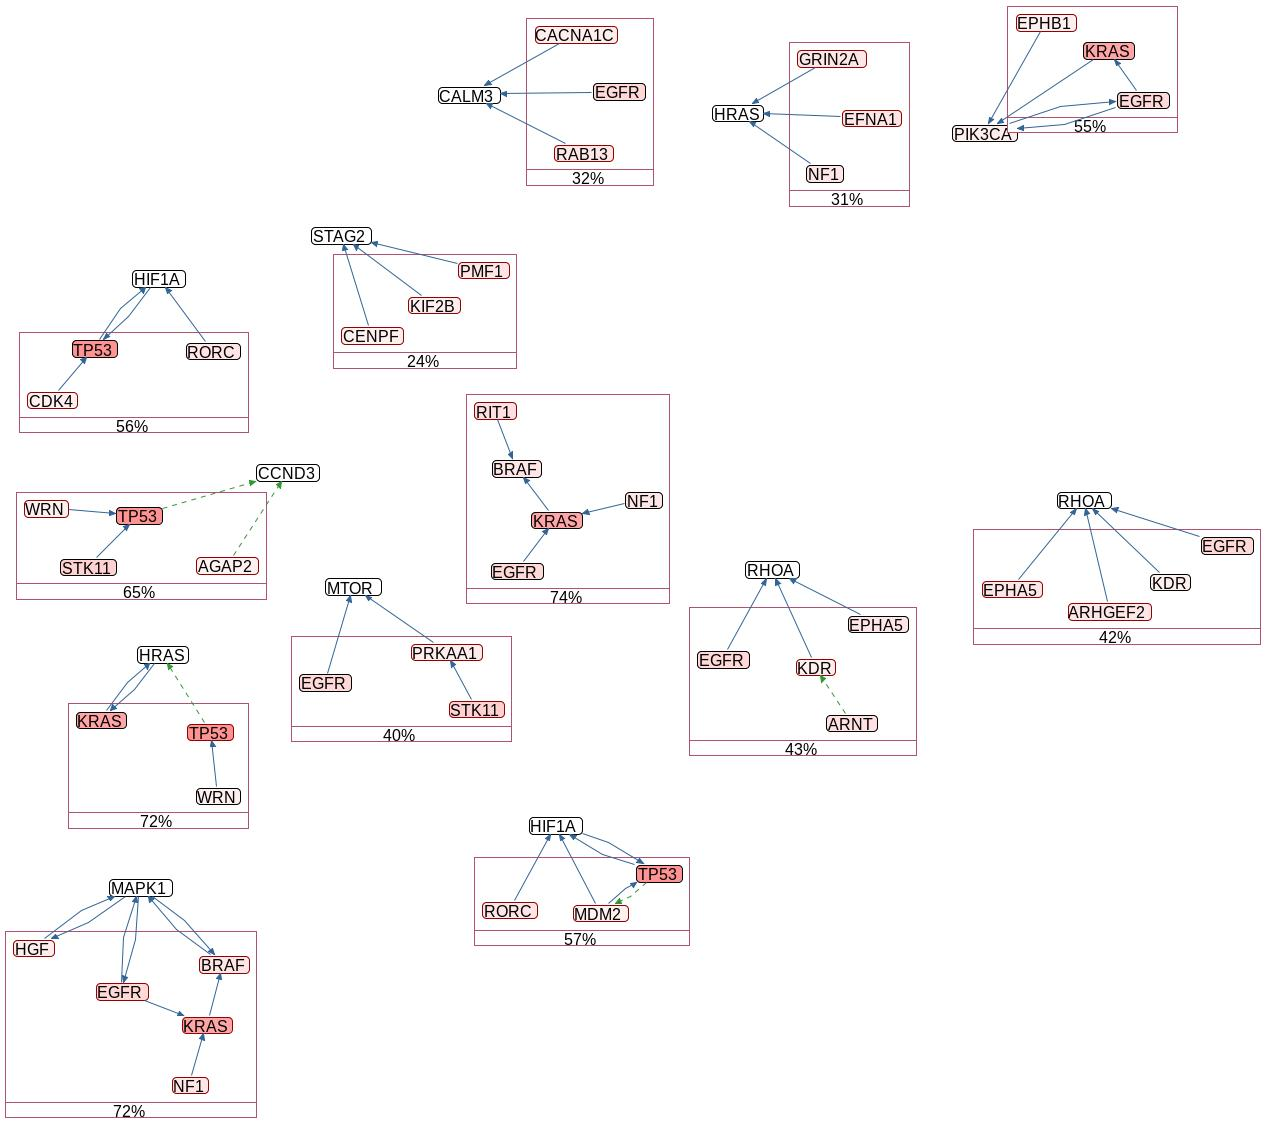
\includegraphics[scale = 0.15]{img/mutexgroup.jpg}
      \caption{Visualization of the exclusivity groups using \textbf{Chisio
          BioPAX Editor (\textit{ChiBE})} \cite{chibe} of the \textit{Mutex}
        results for \textit{LUAD}.}  
    \end{figure}
  }
\end{frame}
\begin{frame}{Mutex II}
  \begin{figure}
    \centering
    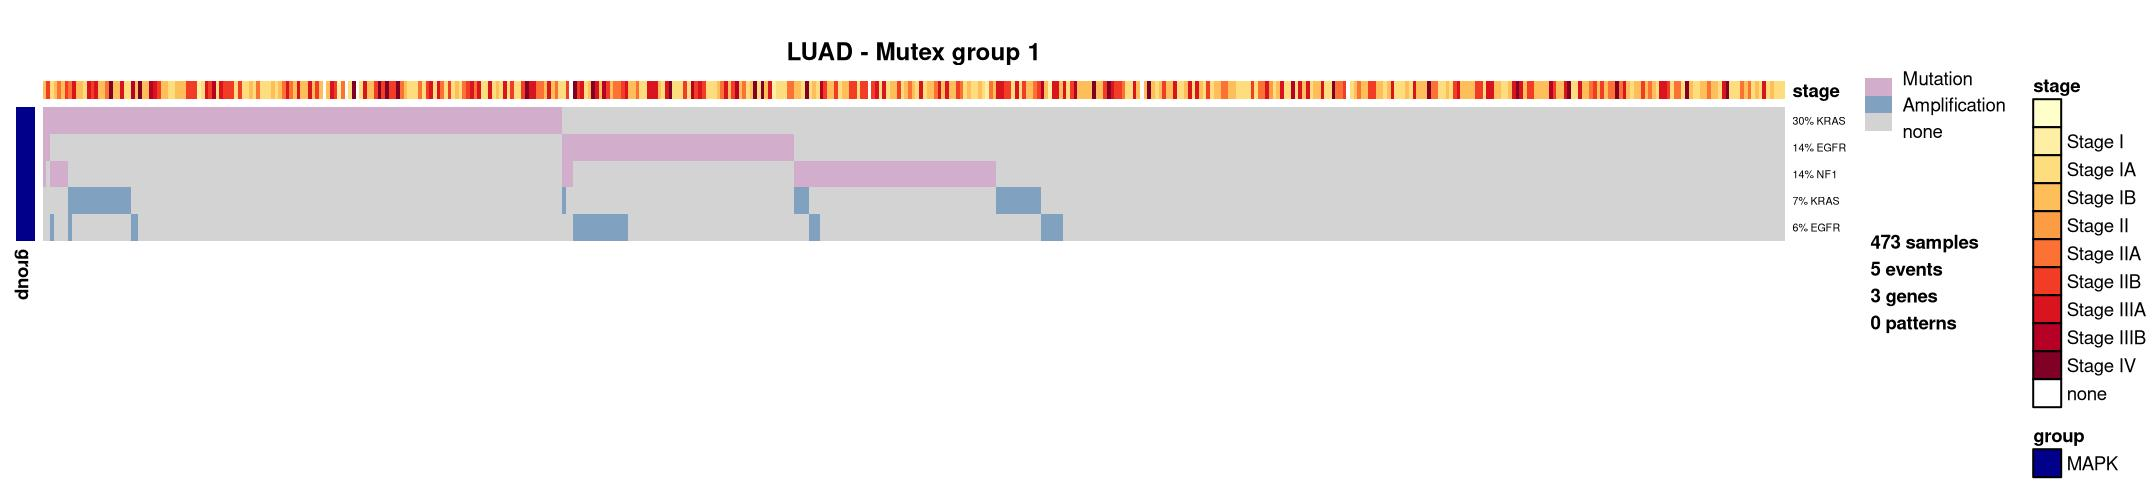
\includegraphics[scale = 0.15]{img/mutex1.jpg}
    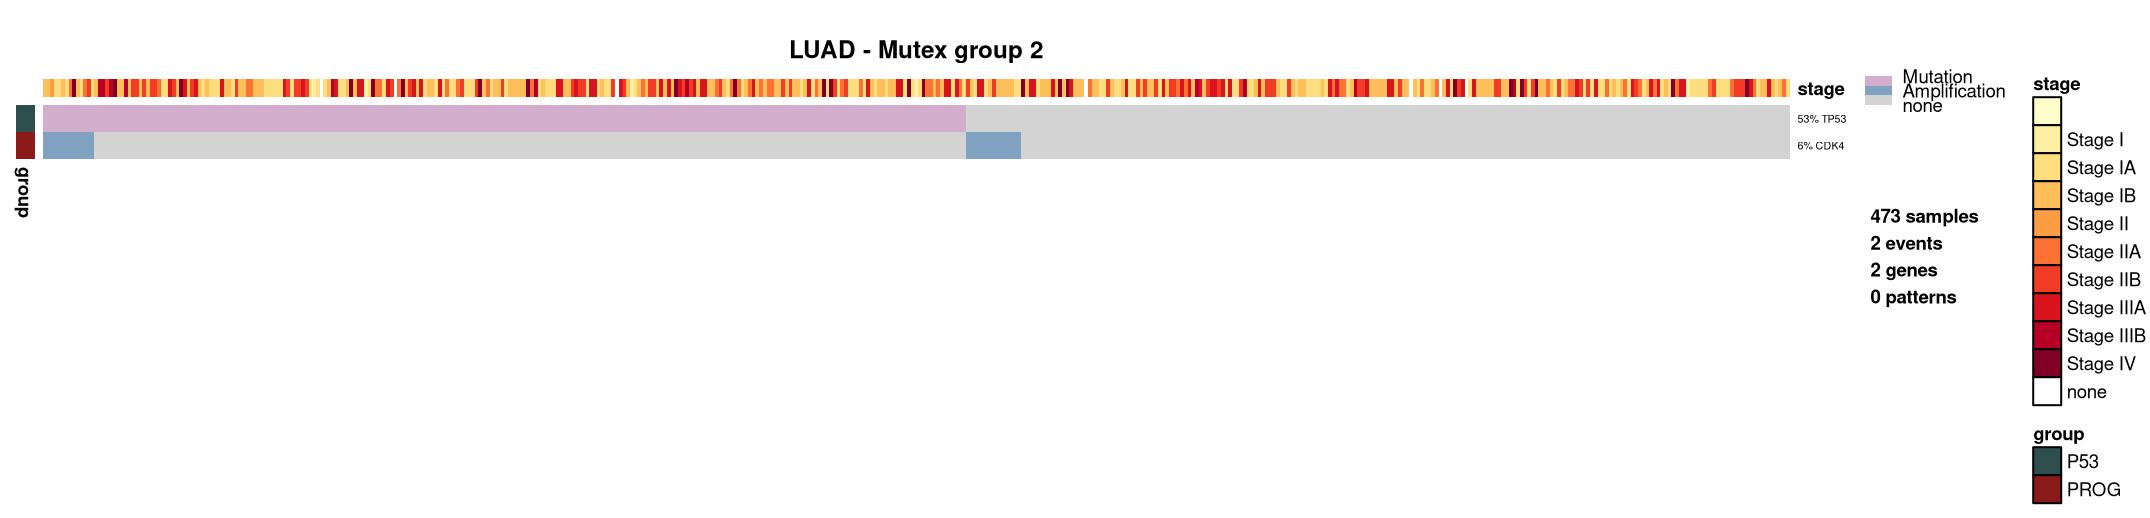
\includegraphics[scale = 0.15]{img/mutex2.jpg}
    \caption{Oncoprint of the first two groups in \textit{Mutex} results for
      \textit{LUAD}.}   
  \end{figure}
\end{frame}
\subsection{Other Hypotheses}
\begin{frame}{MEGSA}
  \begin{block}{}
    In order to have other hypotheses we did a search in the literature, finding
    a paper \cite{megsaluad} on \textit{LUAD} analysis where a tool called
    \textbf{MEGSA} \cite{megsa} was used. We therefore decided to include the
    two annotated hypotheses, as \textbf{OR} hypotheses.  
  \end{block}
  \begin{figure}
    \centering
    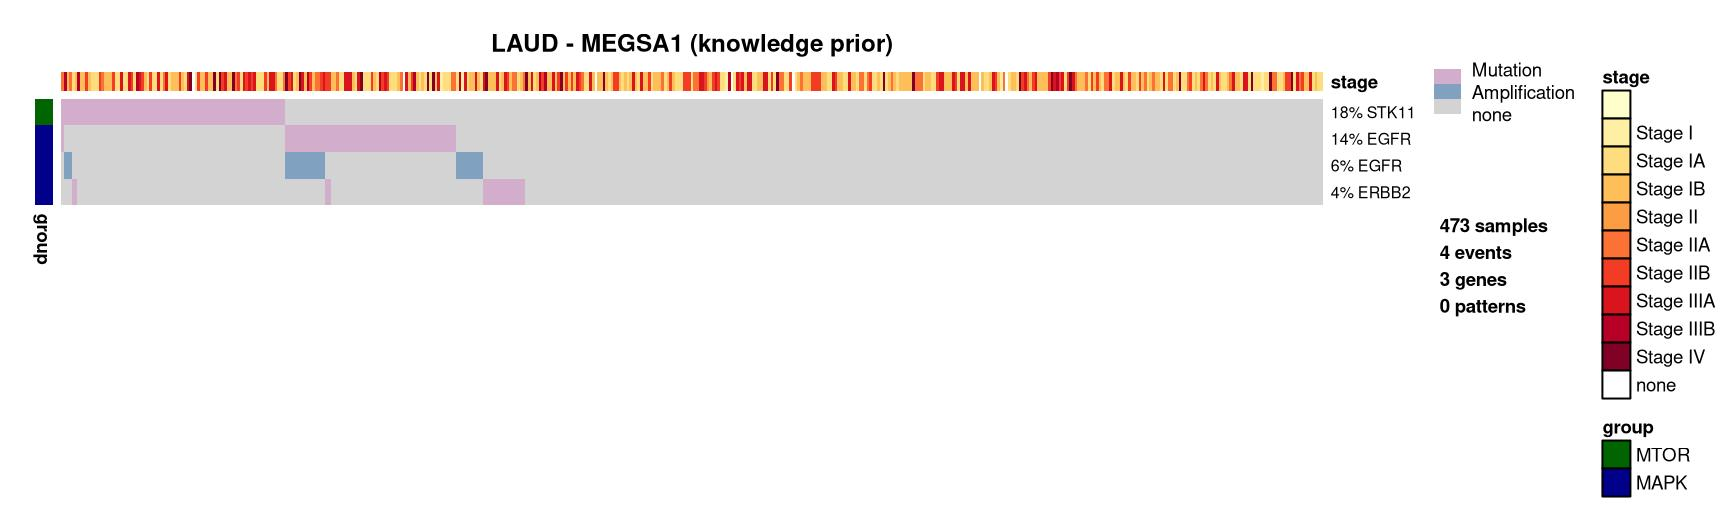
\includegraphics[scale = 0.15]{img/megsa1.jpg}
    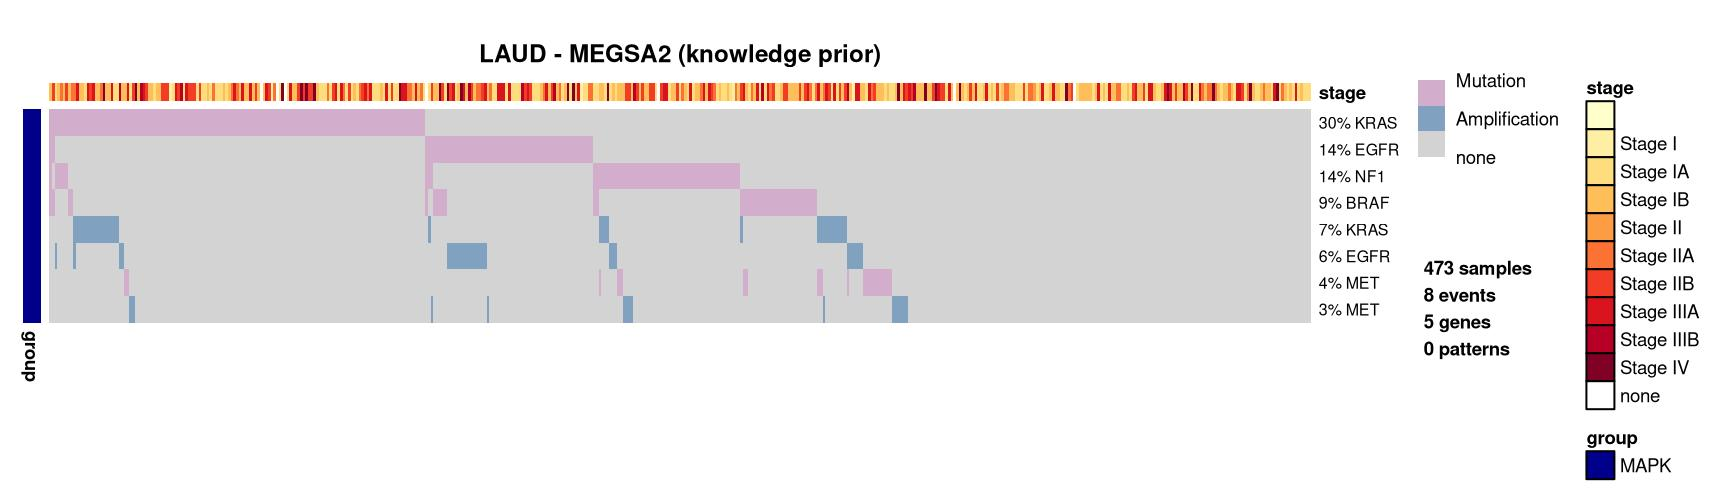
\includegraphics[scale = 0.15]{img/megsa2.jpg}  
  \end{figure}
\end{frame}
\begin{frame}{Marker Paper Hypotheses I}
  \begin{block}{Marker paper Hypothesis}
    Finally we included a hypothesis from the marker paper. Infact we have:\\
    ``\textit{Mutations in KRAS ($33\%$) were mutually exclusive with those in
      EGFR ($14\%$).}'' so we add this as a \textbf{XOR} hypotheses.
  \end{block}
  \begin{figure}
    \centering
    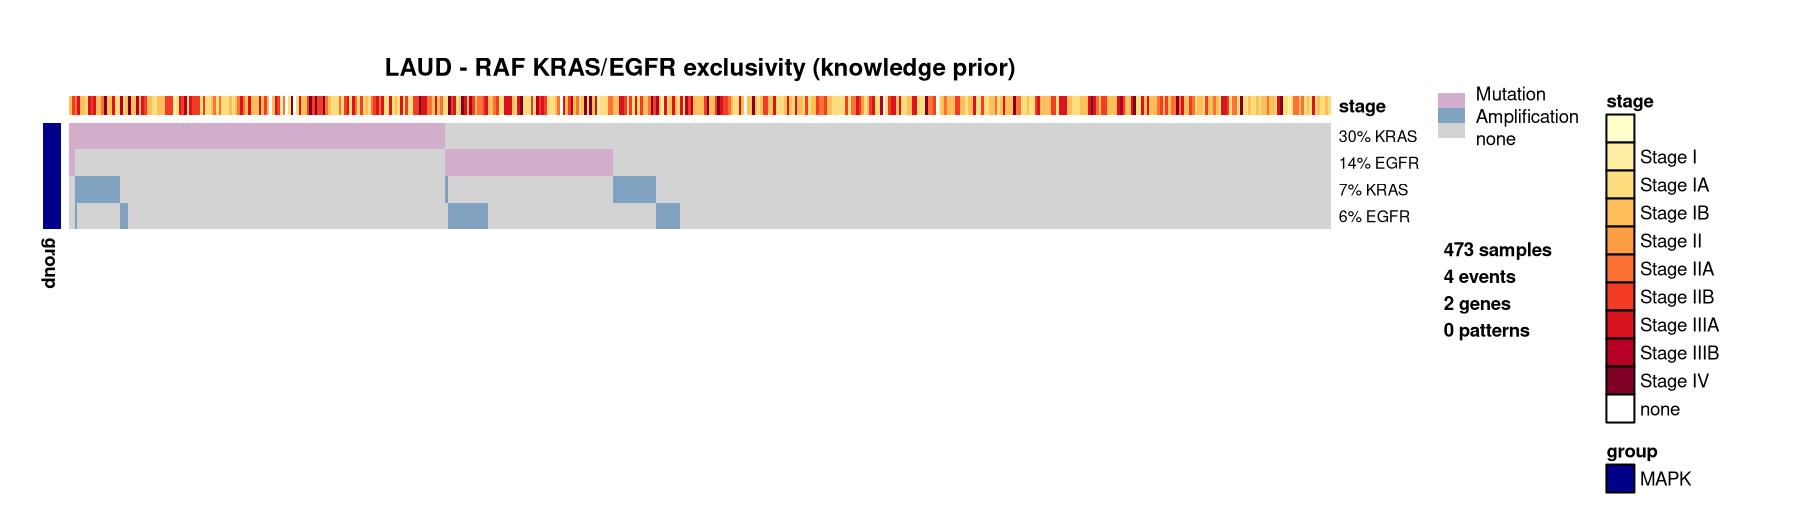
\includegraphics[scale = 0.18]{img/oncoprior.jpg}  
  \end{figure}
\end{frame}
\begin{frame}{Marker Paper Hypotheses II}
  \only<1>{
    \begin{block}{Subtyping Hypotheses}
      For the subtypes we some extra hypotheses based on the marker paper:
      \begin{itemize}
        \item for \textit{PP} subtype we can find in the paper: ``\textit{The PP
          subtype was enriched for mutation of KRAS, along with inactivation of
          the STK11 tumour suppressor gene by chromosomal loss, inactivating
          mutation, and reduced gene expression}'' so we add this as an
        \textbf{AND} hypothesis 
        \item for \textit{PI} subtype we can find in the paper: ``\textit{the PI
          subtype was characterized by solid histopathology and co-mutation of NF1
          and TP53}'' so we add this as an \textbf{AND} hypothesis 
      \end{itemize}
    \end{block}
  }
  \only<2>{
    \begin{figure}
      \centering
      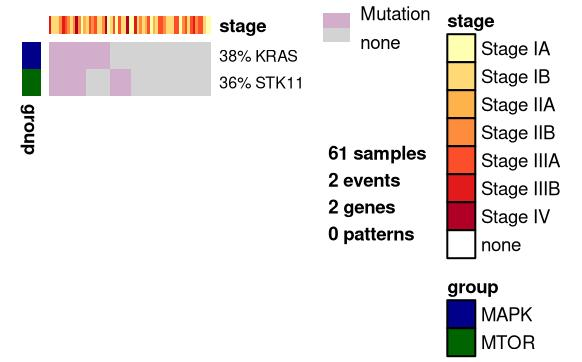
\includegraphics[scale = 0.27]{img/priorsub1.jpg}
      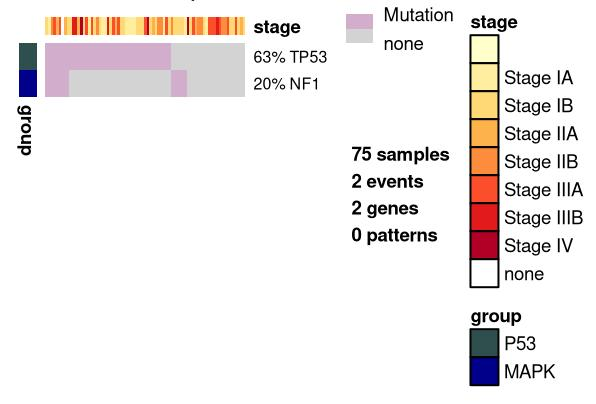
\includegraphics[scale = 0.27]{img/priorsub2.jpg}
      \caption{Oncoprint of the hypotheses for subtypes from the marker paper.}
    \end{figure}
  }
\end{frame}
\section{Model Reconstruction}
\begin{frame}{Models Preparation}
  \begin{block}{}
    Before proceeding with the reconstruction of the cancer progression model
    with the \textbf{CAPRI algorithm} we cleaned up the data: 
    \begin{itemize}
      \item we only kept the genes drivers that are present in the hypotheses
      \item we collapse multiple events per gene in one unique event
      \item we \textit{consolidate} the \textit{TRONCO} object, deleting
      indistinguishable events, having alterations which have the same signature
      across the samples, "programmatically" 
    \end{itemize}
  \end{block}
  \pause
  \begin{block}{}
    Then we added all the hypotheses using \textit{TRONCO} methods, iterating
    over the \textit{Mutex object} and adding all the hardcoded hypotheses
    stated before. Finally we added automatically all the hypotheses related to
    homologous events, using the homonymous function. 
  \end{block}
\end{frame}
\begin{frame}{CAPRI I}
  \begin{block}{}
    \small
    We executed the \textbf{CAPRI algorithm} \cite{capri} almost with default
    settings: 
    \begin{itemize}
      \item \textbf{regularizers} for the likelihood estimation \cite{picnic}:
      \begin{itemize}
        \item \textbf{Akaike Information Criterion (\textit{AIC})}, more prone
        to overfitting but also likely to provide good predictions from data and
        is better when false negatives are more misleading than positive one 
        \item \textbf{Bayesian Information Criterion (\textit{BIC})}, more prone
        to underfitting errors, thus more parsimonious and better in the
        opposite direction. 
      \end{itemize}
      \item \textbf{p-value < 0.05} to accept the valid selective advantage
      relations 
      \item \textbf{heuristic search} is performed with \textit{Hill Climbing}
      \item \textbf{seed} for bootstrap iterations has been set to 42 -
      \textit{the Answer to the Ultimate Question of Life, the Universe, and
        Everything} 
    \end{itemize}
    In addition the \textbf{number of boostrap iterations} is choosen at the
    begin of the pipeline and for this project we use 100 iterations.\\ 
    The details on the labels of the models will be explored further on.
  \end{block}
\end{frame}
\begin{frame}{CAPRI II}
  \only<1>{
    \begin{figure}
      \centering
      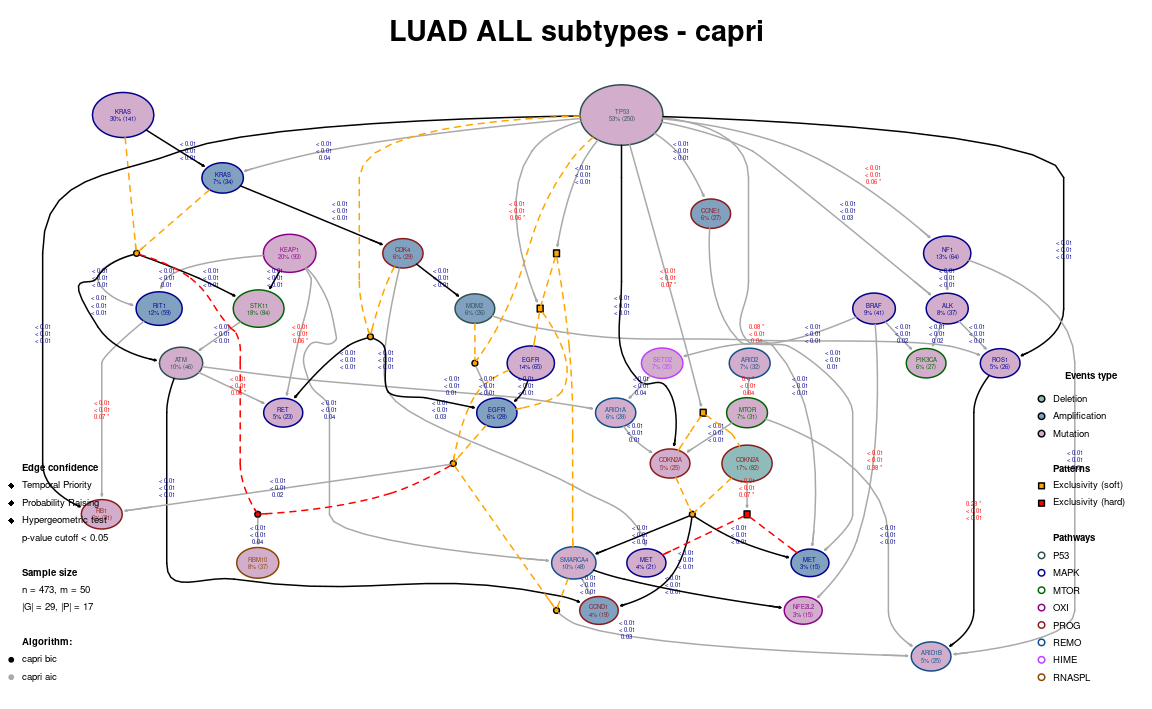
\includegraphics[scale = 0.52]{img/LUAD_all.png}
      \caption{\textit{TRONCO.plot} of the reconstructed model from the data
        including all subtypes.} 
    \end{figure}
  }
  \only<2>{
    \begin{figure}
      \centering
      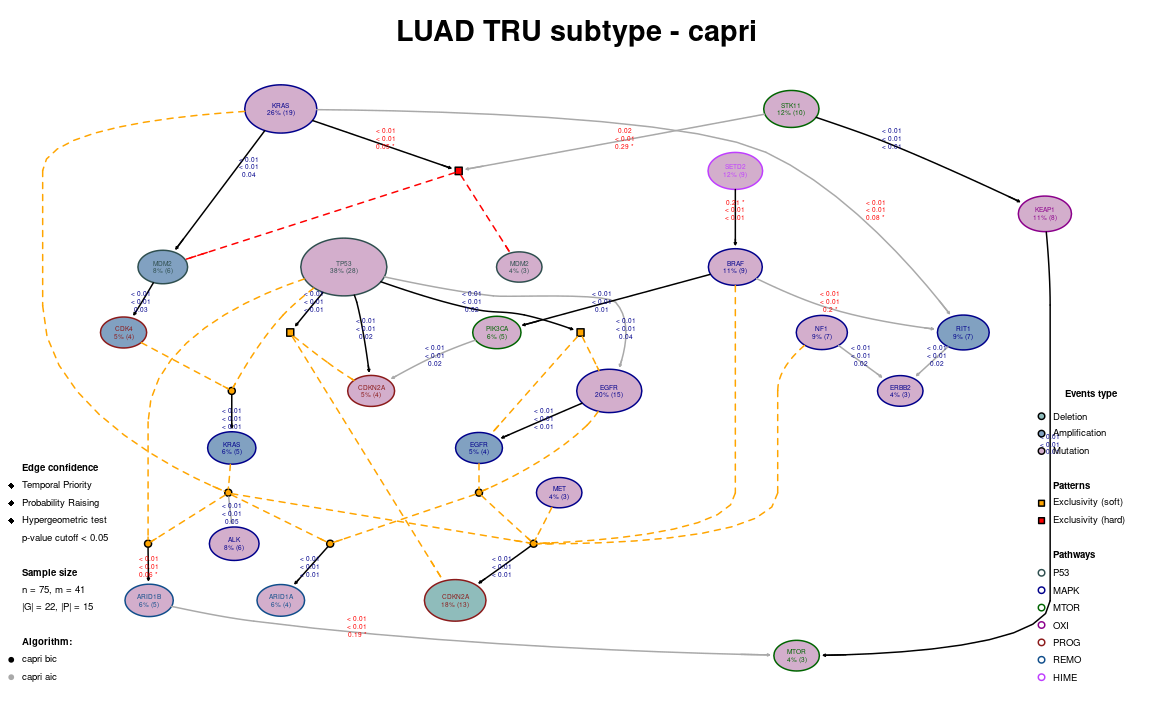
\includegraphics[scale = 0.52]{img/LUAD_tru.png}
      \caption{\textit{TRONCO.plot} of the reconstructed model from the data of
        TRU subtype.} 
    \end{figure}
  }
  \only<3>{
    \begin{figure}
      \centering
      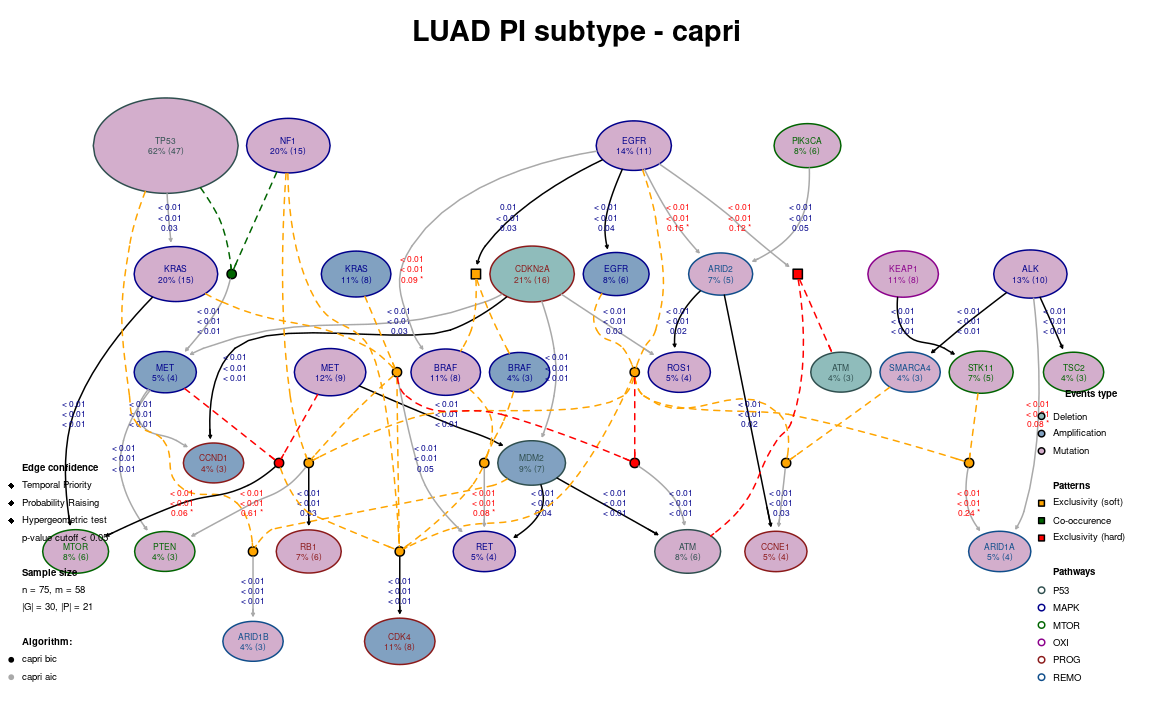
\includegraphics[scale = 0.52]{img/LUAD_pi.png}
      \caption{\textit{TRONCO.plot} of the reconstructed model from the data of
        PI subtype.} 
    \end{figure}
  }
  \only<4>{
    \begin{figure}
      \centering
      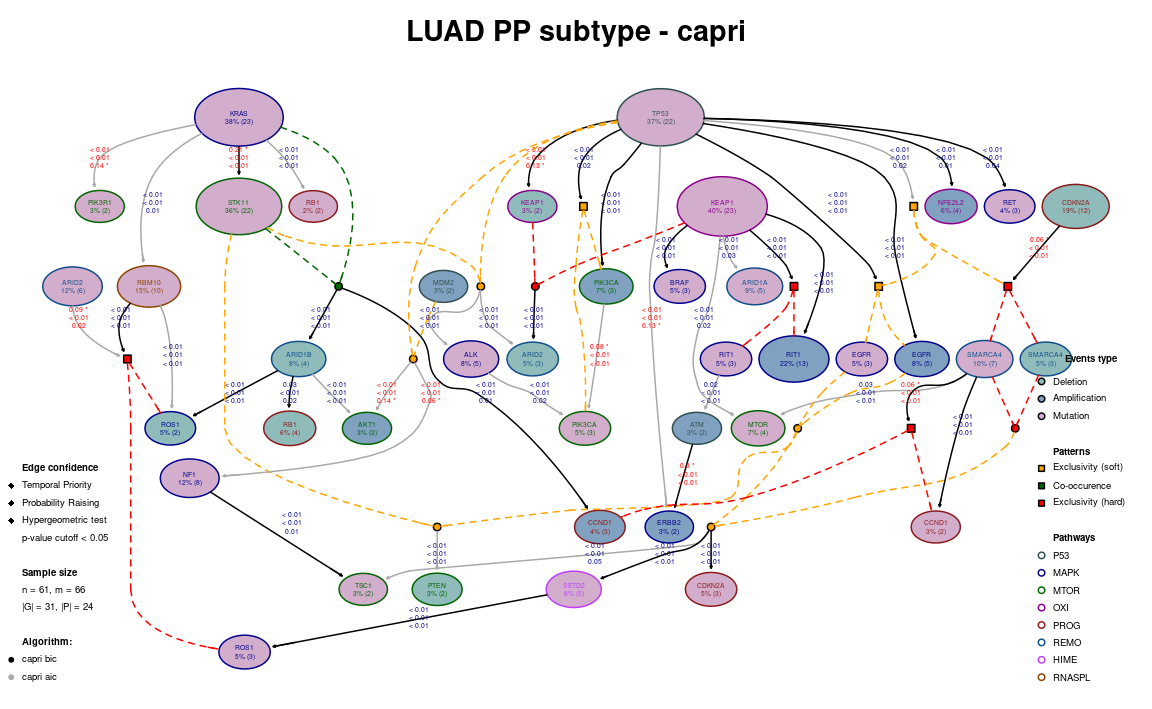
\includegraphics[scale = 0.52]{img/LUAD_pp.png}
      \caption{\textit{TRONCO.plot} of the reconstructed model from the data of
        PP subtype.} 
    \end{figure}
  }
\end{frame}
\begin{frame}{Evolutionary Trajectories I}
  \only<1>{
    \begin{block}{Branching trajectory}
      In this case we have that from one mutation we could have two different
      and independent mutation in different samples (and eventually other
      mutations to follow).\\ 
      In the model we have, for example in PP subtype model, something like
      this: 
    \end{block}
    \begin{figure}
      \centering
      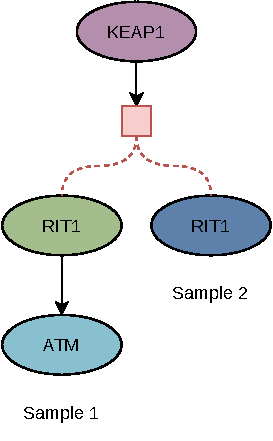
\includegraphics[scale = 0.65]{img/branch.pdf}
    \end{figure}
  }
  \only<2>{
    \begin{figure}
      \centering
      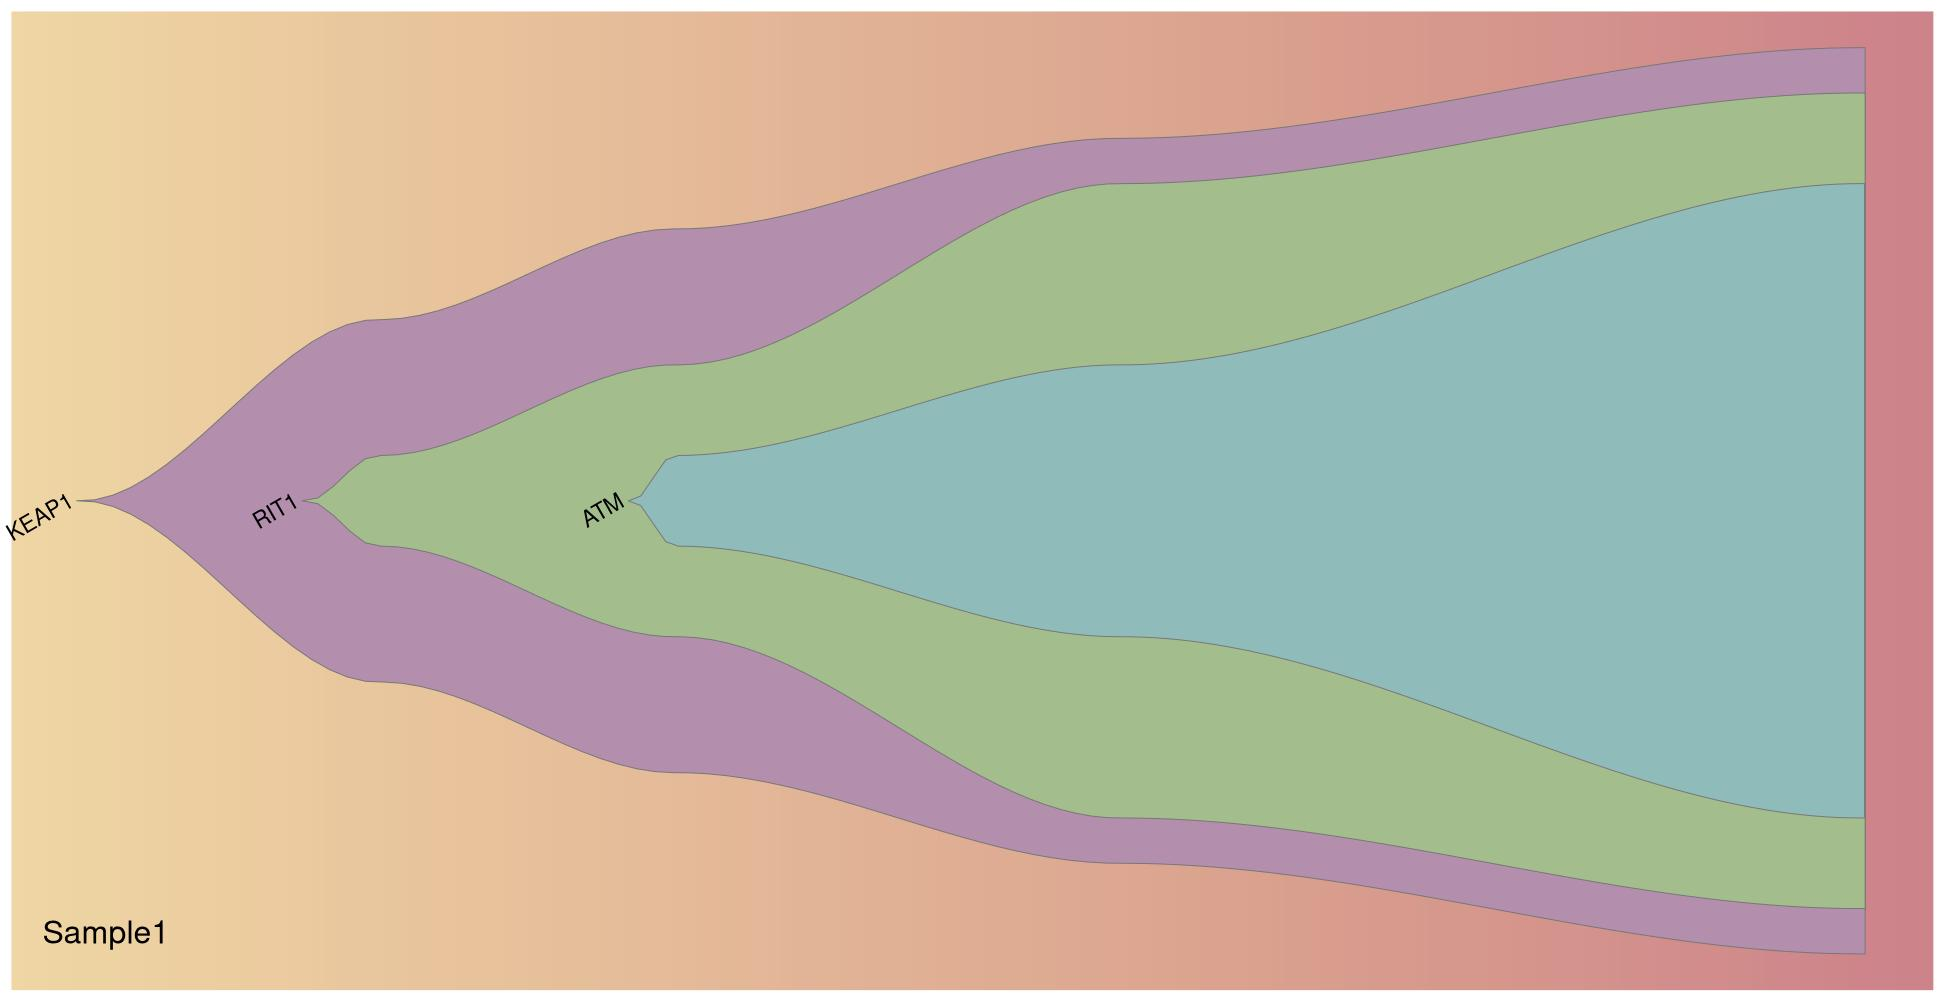
\includegraphics[scale = 0.09]{img/branch1.jpg}
      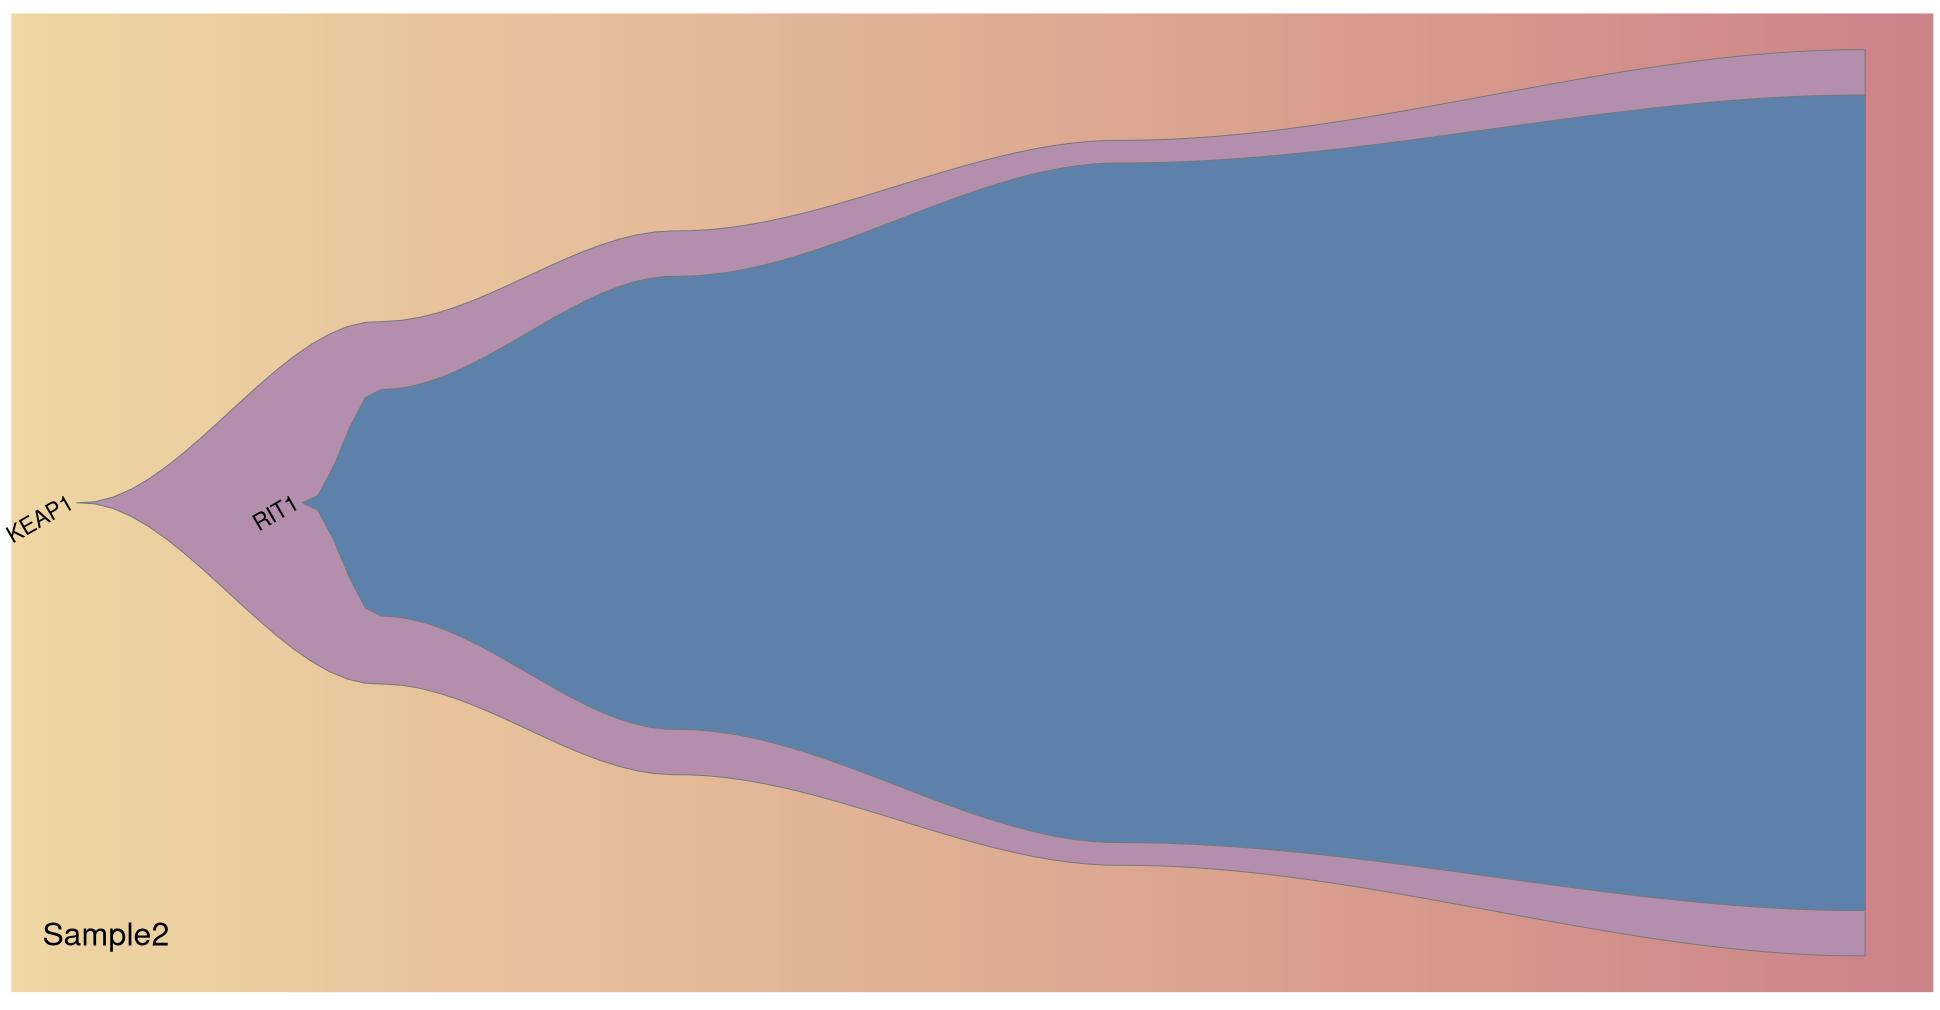
\includegraphics[scale = 0.09]{img/branch2.jpg}
      \caption{Manually curated branching trajectories from PP subtype, plotted
        using \textit{Fishplot library} \cite{fishplot}.} 
    \end{figure}
  }
\end{frame}
\begin{frame}{Evolutionary Trajectories II}
  \only<1>{
    \begin{block}{Branching trajectory}
      In this case we have that from two different mutation paths we converge to
      the same mutation.\\ 
      In the model we have, for example in PP subtype model, something like
      this: 
    \end{block}
    \begin{figure}
      \centering
      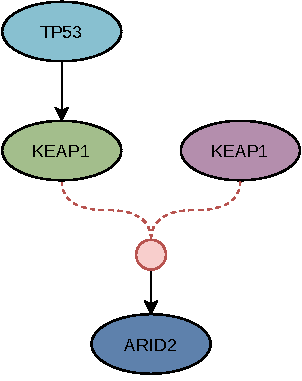
\includegraphics[scale = 0.65]{img/confluence.pdf}
    \end{figure}
  }
  \only<2>{
    \begin{figure}
      \centering
      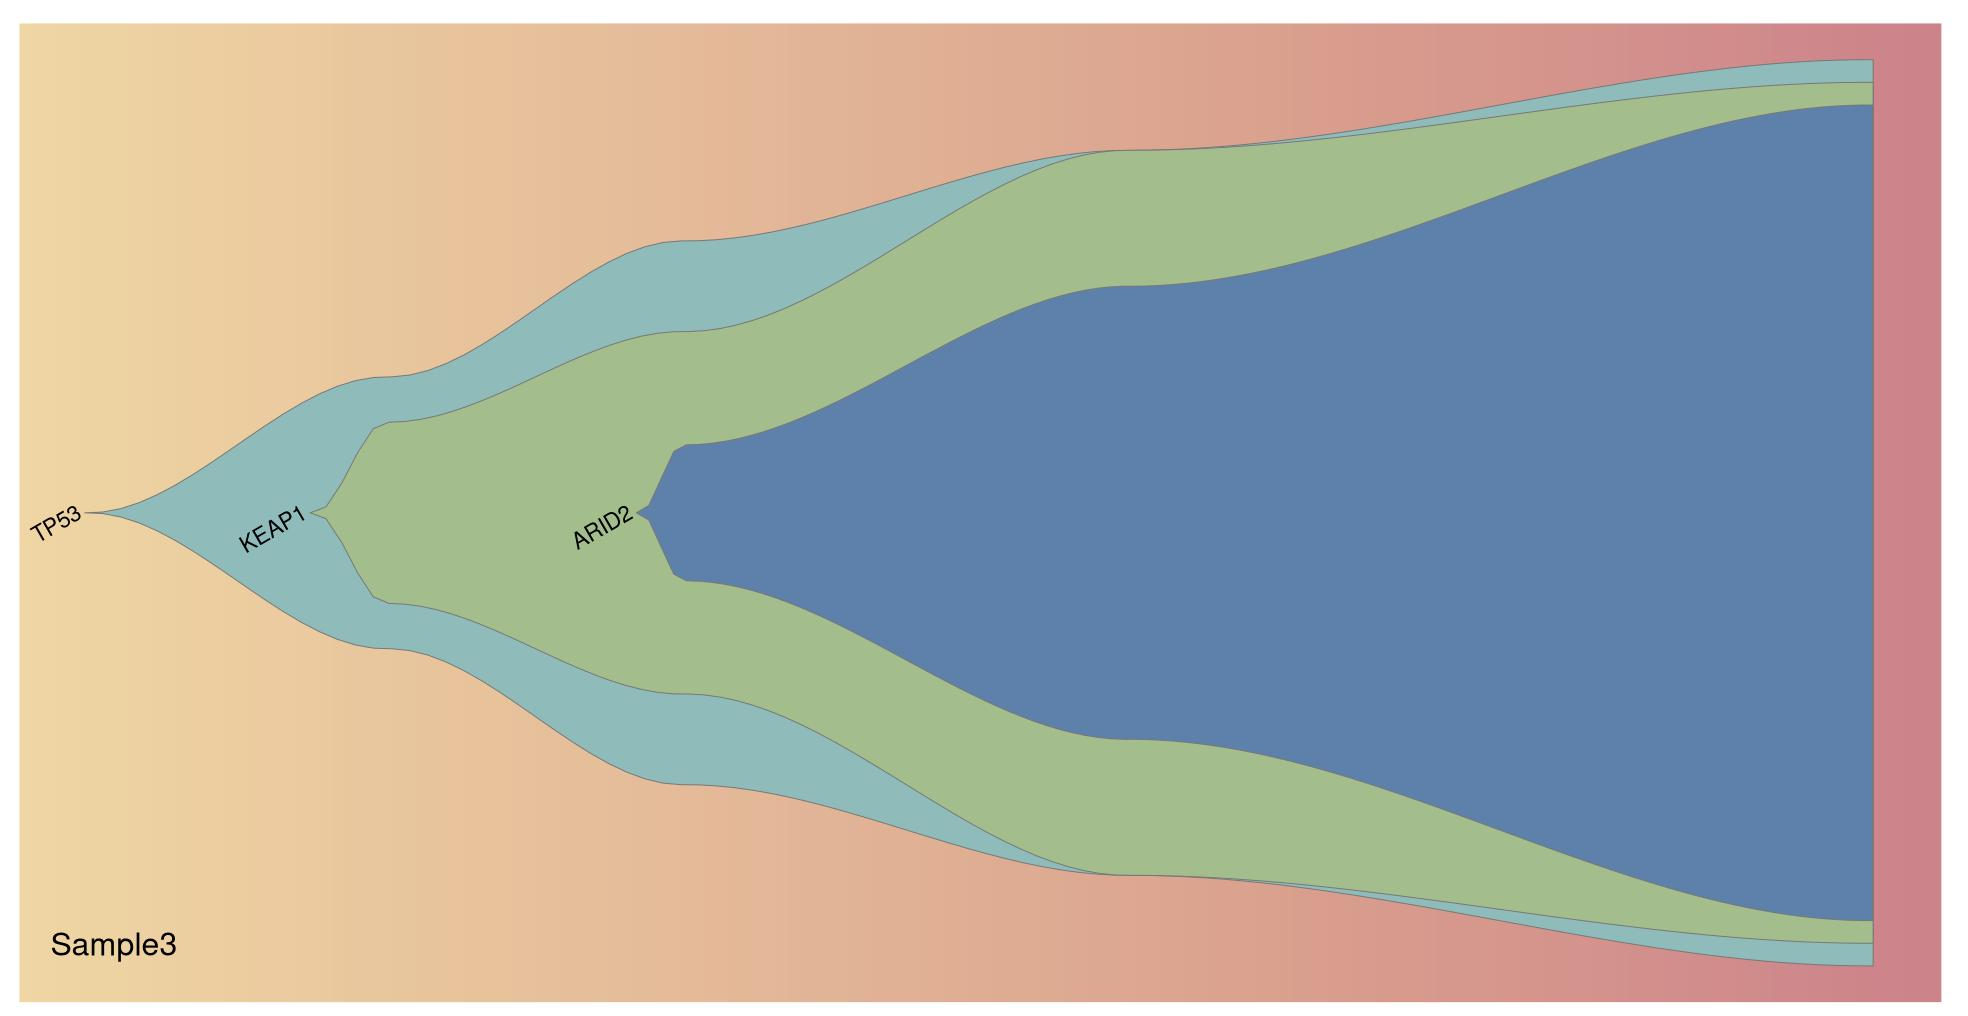
\includegraphics[scale = 0.09]{img/confluence1.jpg}
      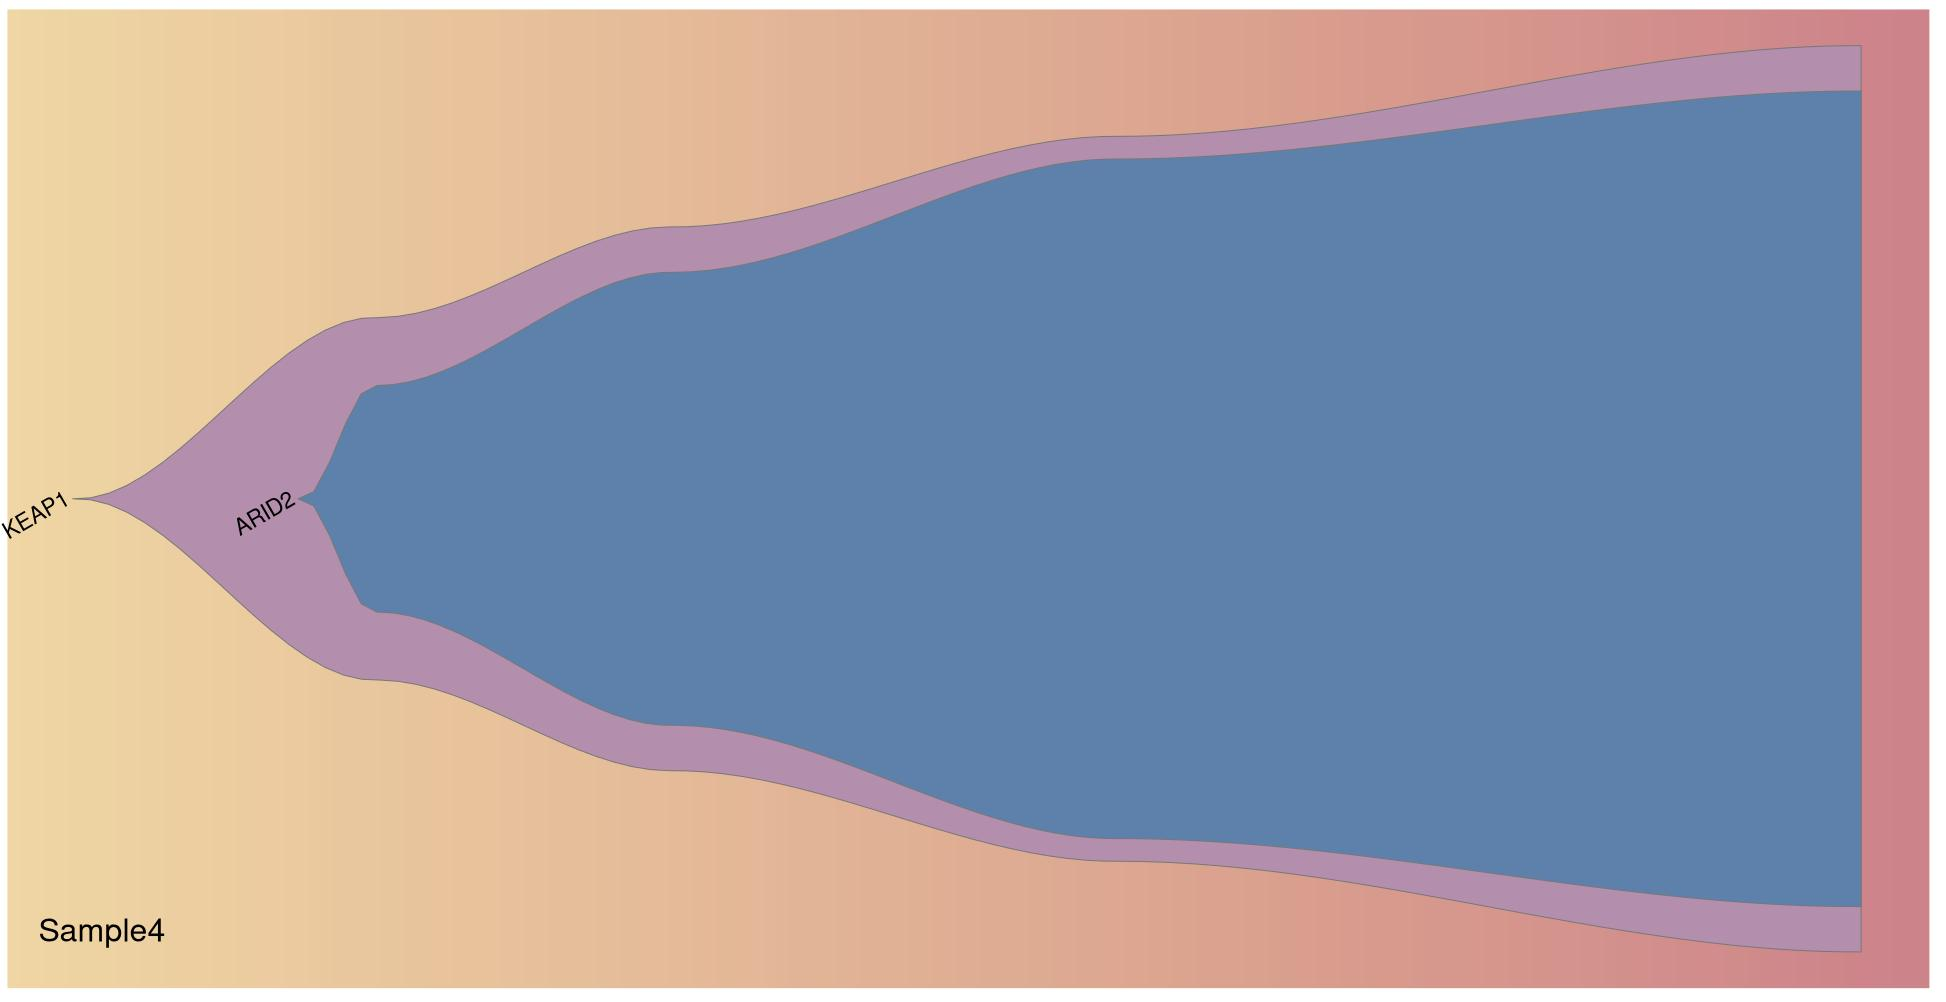
\includegraphics[scale = 0.09]{img/confleunce2.jpg}
      \caption{Manually confluencing trajectories from PP subtype, plotted using
        \textit{Fishplot library} \cite{fishplot}.} 
    \end{figure}
  }
\end{frame}
\section{Statistical Analysis}
\begin{frame}{Post-Reconstruction I}
  \begin{block}{}
    We calculated some scores:
    \begin{itemize}
      \item \textbf{non-parametric boostrap scores} resampling the dataset,
      re-running \textit{CAPRI algorithm} and computing the scores based on how
      many times we re-infer the same edge 
      \item \textbf{statistical bootstrap scores}, re-running the statistical
      test for temporal priority and probability raising by initializing a
      random number generator with different seeds  
    \end{itemize}
  \end{block}
  \pause
  \begin{block}{}
    As we'll see later, the scores obtained in our analysis seem to validate the
    goodness of our models. 
  \end{block}
\end{frame}
\begin{frame}{Post-Reconstruction II}
  \begin{figure}
    \centering
    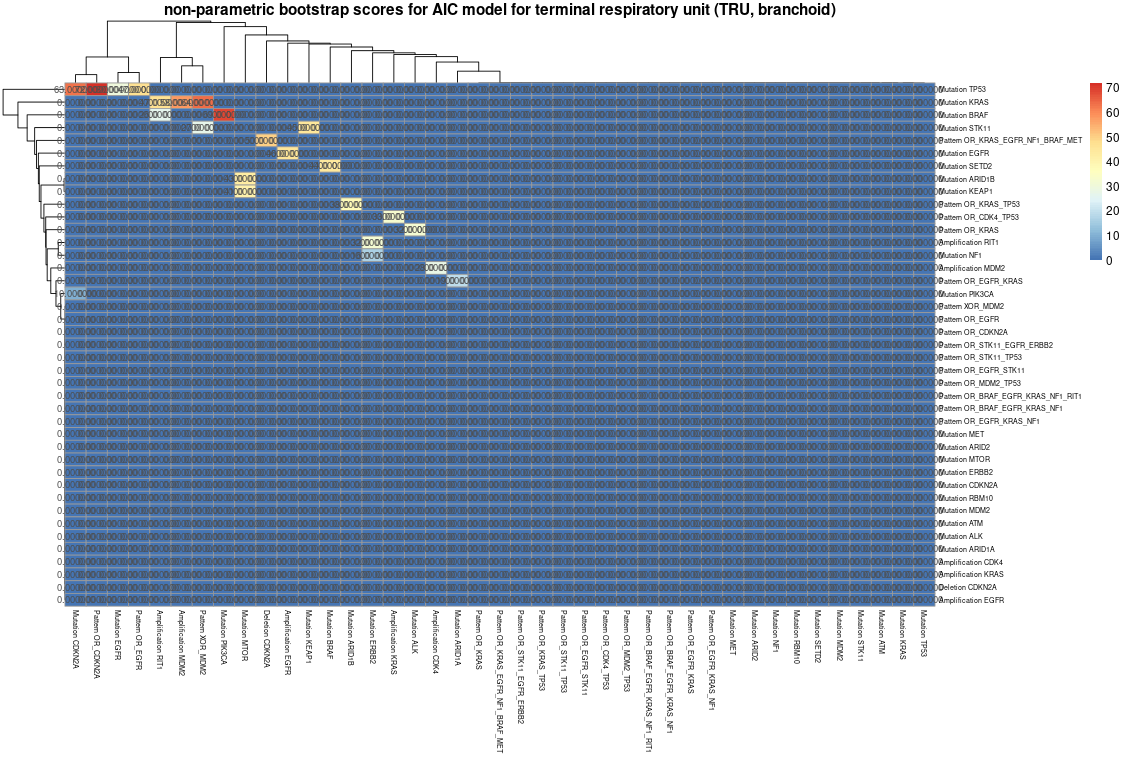
\includegraphics[scale = 0.27]{img/TRU_heat.png}
    \caption{Example of Non Parametric and Statistical results shown as heatmap
      for AIC bootstrap scores for TRU subtype model.} 
  \end{figure}
\end{frame}
\begin{frame}{Post-Reconstruction III}
  \only<1>{
    \begin{block}{Edge labels}
      \scriptsize
      Given an event $c$ and an event $e$, at time $t_c$ and $t_e$, with
      $0<Pr(c),\,Pr(e)<1$: 
      \begin{itemize}
        \item \textbf{temporal priority}, \textit{p-value} of temporal priority,
        $t_c < t_e$, via \textit{Mann-Whitney U testing}
        \item \textbf{probability raising}, \textit{p-value} of probability
        raising, $Pr(e|\neg c)<Pr(e|c)$, via \textit{Mann-Whitney U testing} 
        \item \textbf{hypergeometric test}, is used to underline if there is a
        difference between samples containing $c \land e$ versus the total
        population of samples containing $c \lor e$. We would like the overlap
        (joint probability of $c$ and $e$) to be significant as this supports
        the presence of a selection trend among $c$ and $e$
      \end{itemize}
      
      An edge is fully supported if all those three p-values are below a
      significance threshold set at 0.05. Some edges might have p-value for the
      \textit{temporal priority} above the threshold, meaning there's still a
      significant selection trend but with a direction (i.e. the temporal order
      of $c$ and $e$) not supported by the data \cite{picnic}. 
    \end{block}
  }
  \only<2>{
    \begin{figure}
      \centering
      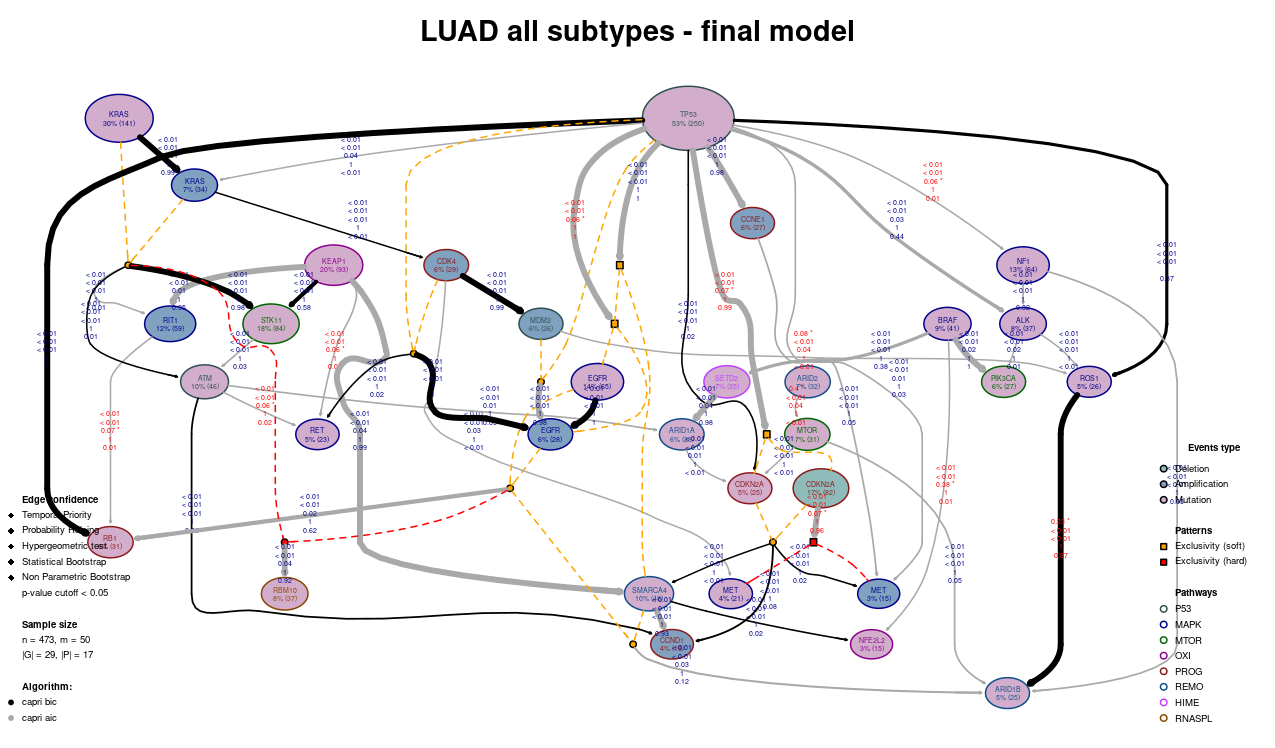
\includegraphics[scale = 0.47]{img/LUAD_ALL_boot.png}
      \caption{\textit{TRONCO.plot} with bootstrap scores of the reconstructed
        model from the data including all subtypes. Edge size represents
        non-parametric bootstrap scores.} 
    \end{figure}
  }
  \only<3>{
    \begin{figure}
      \centering
      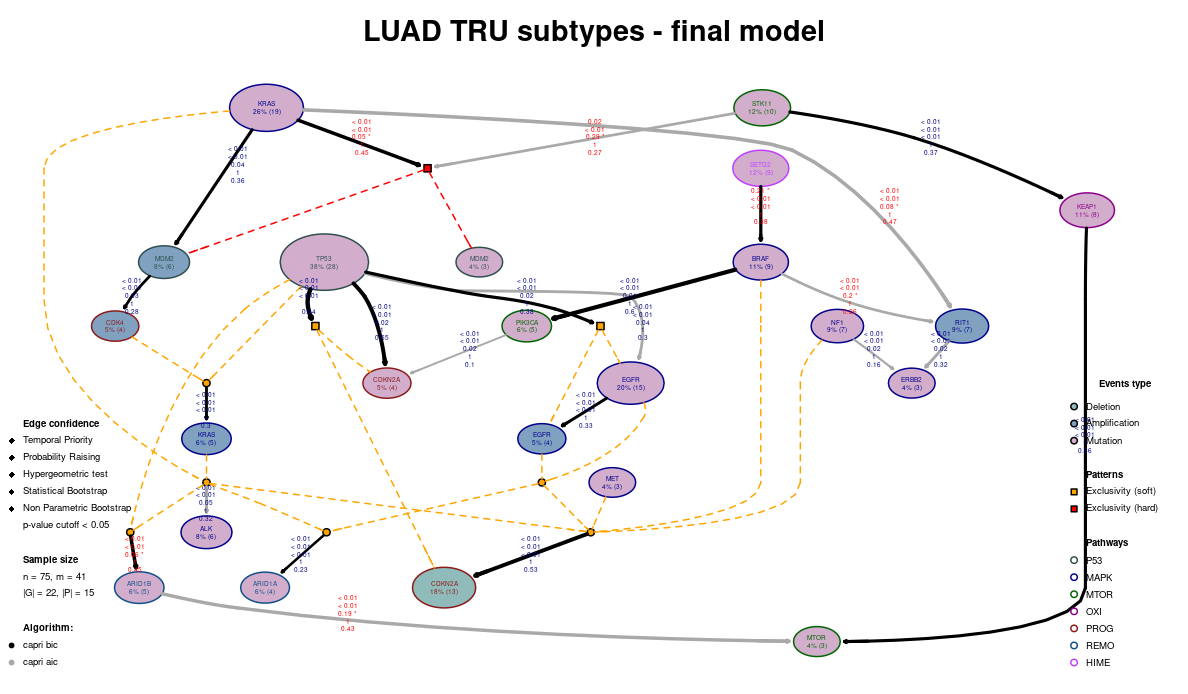
\includegraphics[scale = 0.50]{img/LUAD_TRU_boot.png}
      \caption{\textit{TRONCO.plot} with bootstrap scores of the reconstructed
        model from the data of TRU subtype. Edge size represents non-parametric
        bootstrap scores.} 
    \end{figure}
  }
  \only<4>{
    \begin{figure}
      \centering
      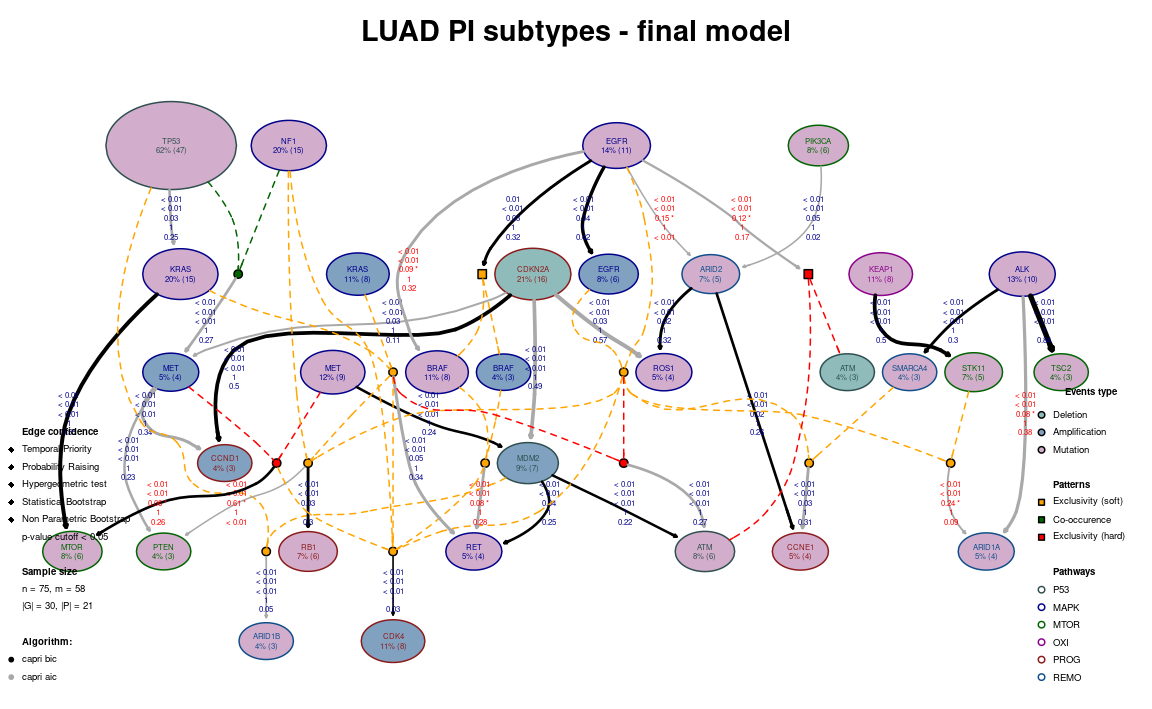
\includegraphics[scale = 0.52]{img/LUAD_PI_boot.png}
      \caption{\textit{TRONCO.plot} with bootstrap scores of the reconstructed
        model from the data of PI subtype. Edge size represents non-parametric
        bootstrap scores.} 
    \end{figure}
  }
  \only<5>{
    \begin{figure}
      \centering
      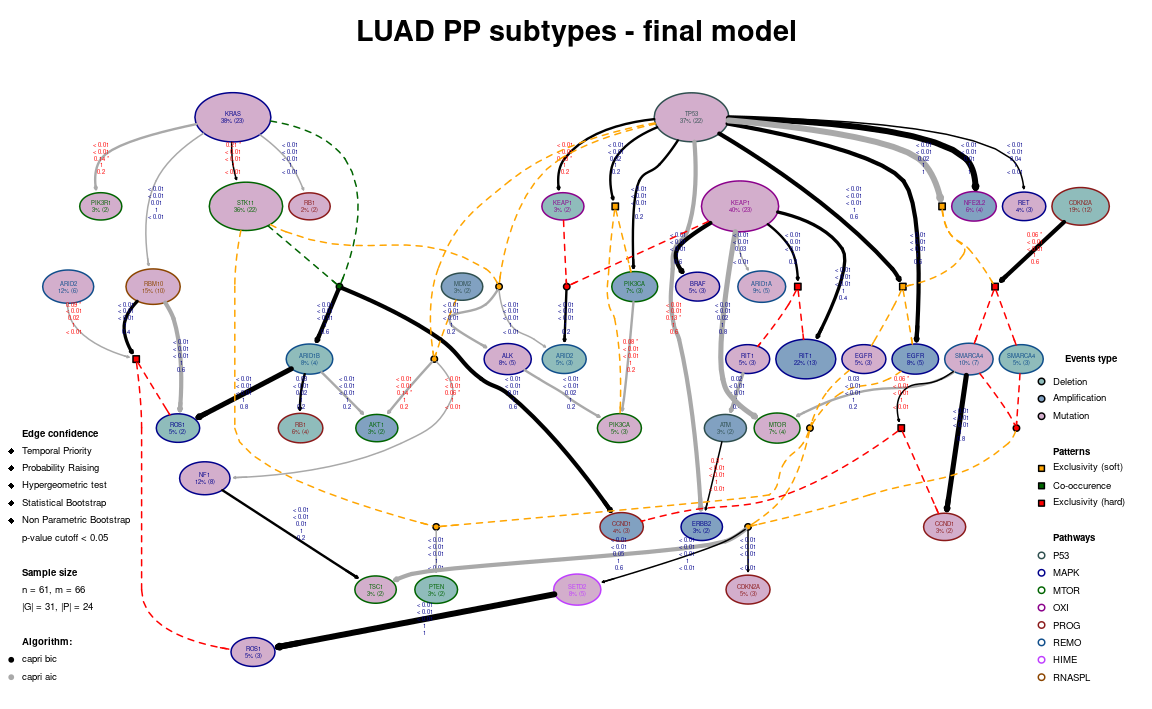
\includegraphics[scale = 0.52]{img/LUAD_PP_boot.png}
      \caption{\textit{TRONCO.plot} with bootstrap scores of the reconstructed
        model from the data of PP subtype. Edge size represents non-parametric
        bootstrap scores.} 
    \end{figure}
  }
\end{frame}
\begin{frame}{10-Fold Cross Validation}
  \only<1>{
    \begin{block}{}
      Then we perform a \textbf{10-fold cross validation} (with 10 iterations)
      studying using the methods included in \textit{TRONCO library}: 
      \begin{itemize}
        \item the \textbf{entropy-loss} for each model computed, that's the
        negated expected log-likelihood of the test set for the Bayesian network
        fitted from the training set 
        \item the \textbf{prediction error} for each parent set of a certain
        node 
        \item the \textbf{posterior classification error} for each edge that
        connect a node to a child 
      \end{itemize}
      These studies have been performed both for \textit{CAPRI AIC models} and
      \textit{CAPRI BIC models}, producing good results. 
    \end{block}
  }
  \only<2>{
    \begin{figure}
      \centering
      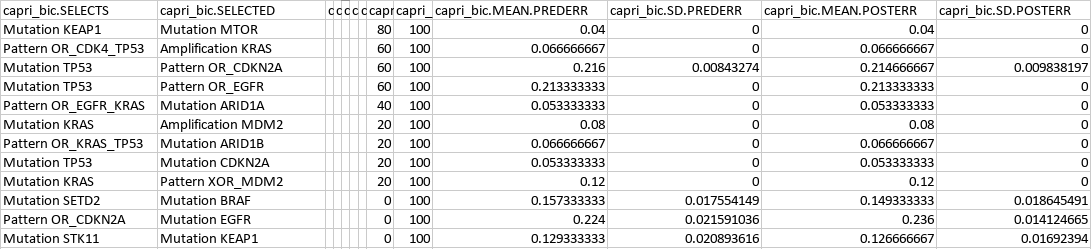
\includegraphics[scale = 0.3]{img/stat_table.png}
      \caption{Example of data extracted from 10-fold cross validation.}
    \end{figure}
  }
\end{frame}
\begin{frame}{Entropy Loss}
  \begin{figure}
    \centering
    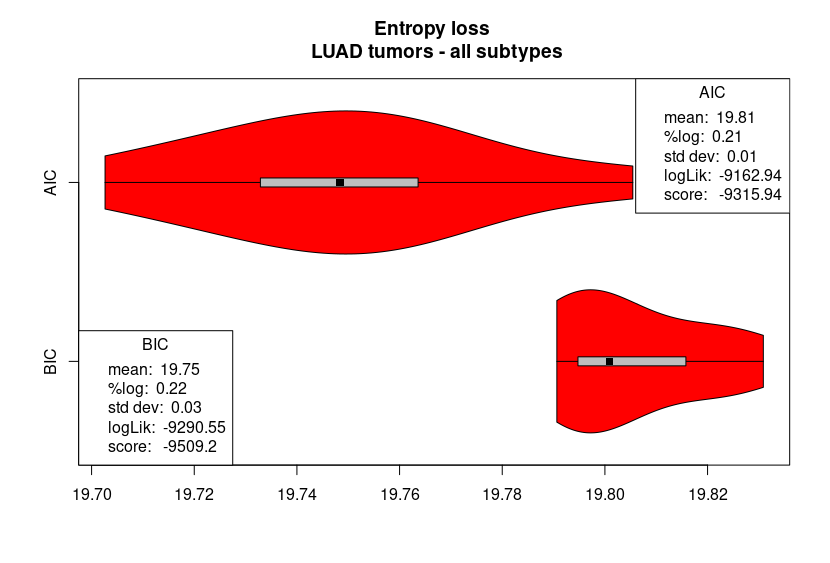
\includegraphics[scale = 0.215]{img/vioplot_ALL.png}
    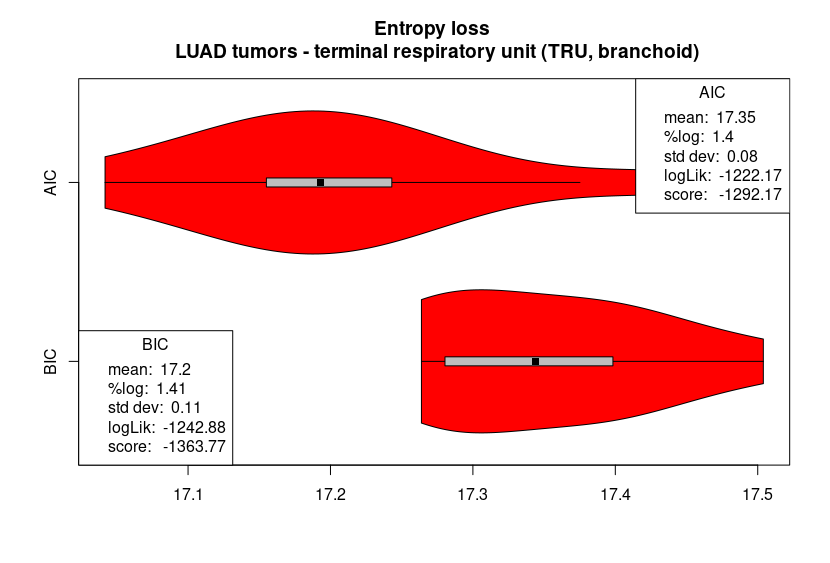
\includegraphics[scale = 0.215]{img/vioplot_TRU.png}
  \end{figure}
  \begin{figure}
    \centering
    \includegraphics[scale = 0.215]{img/vioplot_PI.png}
    \includegraphics[scale = 0.215]{img/vioplot_PP.png}
    \caption{Violin plot, obtained by Vioplot \cite{vioplot}, for entropy loss
      of all models.} 
  \end{figure}
\end{frame}
\begin{frame}{Prediction Error}
  \only<1>{
    \begin{figure}
      \centering
      \includegraphics[scale = 0.38]{img/prederr_aic_PP.png}
      \caption{Barplot of prediction error of AIC model for PP subtype
        reconstruction.} 
    \end{figure}
  }
  \only<2>{
    \begin{figure}
      \centering
      \includegraphics[scale = 0.38]{img/prederr_bic_PP.png}
      \caption{Barplot of prediction error of BIC model for PP subtype
        reconstruction.} 
    \end{figure}
  }
\end{frame}
\begin{frame}{Posterior Classification}
  \only<1>{
    \begin{figure}
      \centering
      \includegraphics[scale = 0.315]{img/post_aic_PP.png}
      \includegraphics[scale = 0.315]{img/post_aic_PP2.png}
      \caption{Posterior classification ($\mu$ and $\sigma$) of AIC model for PP
        subtype reconstruction.} 
    \end{figure}
  }
  \only<2>{
    \begin{figure}
      \centering
      \includegraphics[scale = 0.4]{img/post_bic_PP.png}
      \caption{Posterior classification ($\mu$ and $\sigma$) of BIC model for PP
        subtype reconstruction.} 
    \end{figure}
  }
  
\end{frame}
\section{Result and Discussion}
\begin{frame}{Result Analysis I}
  % TODO inserire robe e fingersi oncologi 
  \begin{block}{}
    From a broad analysis of the results we can see in each model the presence
    of mutations for \textit{TP53}, primarily responsible for apoptosis. 
  \end{block}
  \pause
  \begin{block}{}
    Another recurrent result is \textit{KEAP1} mutation which concerns the
    response to oxidative stress. 
  \end{block}
  \pause
  \begin{block}{}
    Finally, there are frequent mutations concerning the genes of the
    \textit{Ras family}, which also have regulatory functions of apoptosis, and
    genes of the \textit{Raf family} that are related to oncogenes and
    participate in \textit{RAS-RAF-MEK-ERK signal transduction cascade}. These
    results seem to be consistent with what is present in the literature
    \cite{rasl}. 
  \end{block}
\end{frame}
\begin{frame}{Result Analysis II}
  \begin{block}{Molecular subtypes}
    Regarding the three subtypes we can observe in the models that the
    hypotheses extracted from the marker paper are represented
    \cite{luadmarker}: 
    \begin{itemize}
      \item "the PI subtype was characterized by solid histopathology and
      co-mutation of \textit{NF1} and \textit{TP53}" 
      \item "the PP subtype was enriched for mutation of \textit{KRAS}, along
      with inactivation of the \textit{STK11} tumour suppressor gene" 
    \end{itemize}
    On the other hand, for TRU subtype, in the marker paper we have: "the TRU
    subtype harboured the majority of the \textit{EGFR-mutated} tumours as well
    as the kinase fusion expressing tumours". This could be confirmed in the
    \textit{DAG} due to the presence of genes mutations from \textit{RAF/RAS
      families}, in addition to \textit{EGFR} mutations. 
  \end{block}
\end{frame}
\begin{frame}{OncoBN Comparison I}
  \only<1>{
    \begin{block}{}
      Trying to validate our results we searched the literature for further
      studies on \textit{LUAD} and one of them is another \textit{R} library
      called \textbf{OncoBN} \cite{oncobn}.\\ 
      In the paper there are also some comparisons with \textit{CAPRI algorithm}
    \end{block}
    
    \begin{block}{}
      In this study the authors recovered three highconfident roots:
      \textit{KRAS}, \textit{KEAP1} and \textit{EGFR} plus a high confident edge
      \textit{TP53}$\to$\textit{RB1}. 
    \end{block}
    
    \begin{block}{}
      From a quick visual comparison, the model obtained with \textit{OncoBN}
      seems consistent with our model obtained from the \textit{PiCnIc pipeline}
      (with all subtypes), even if the latter takes into account a much more
      complex input which involves an equally complex final model. 
    \end{block}
  }
  \only<2>{
    \begin{figure}
      \centering
      \includegraphics[scale = 0.75]{img/oncobn.jpg}
      \caption{Synthetically lethal mutations of \textbf{LUAD}, \textit{KRAS}
        and \textit{EGFR} ({\color{nordgreen}green nodes}), appear in disjoint
        branches. Frequently co-occurred mutations \textit{STK11},
        \textit{KEAP1} and \textit{SMARCA4} occupy a branch of the inferred
        network ({\color{nordred}red nodes}). Subtype defining mutations
        \textit{TP53} and \textit{RB1} are ordered with high confident
        \cite{oncobn}.} 
    \end{figure}
  }
\end{frame}
\begin{frame}{OncoBN Comparison II}
  \begin{block}{Comparison with \textit{PiCnIc models}}
    \begin{itemize}
      \item \textbf{All subtypes}: all the edges and nodes can be found in
      \textit{CAPRI} model  
      \item \textbf{TRU subtype}: we can't find any edge but we have some
      consistent nodes 
      \item \textbf{PI subtype}: we can't find any edge, except
      \textit{KEAP1}$\to$\textit{STK11}, but we have some consistent nodes 
      \item \textbf{PP subtype}: we have some consistent edges but it has all
      nodes. It's interesting to report that \textit{TP53} is strongly related
      with some mutations, with few samples, that are not shown in
      \textit{OncoBN} plot. 
    \end{itemize}
  \end{block}
  \begin{block}{}
    These can be considered expected results due to the fact that
    \textit{OncoBN} does not study mutational subtypes.   
  \end{block}
\end{frame}
\section{References and Q\&A}
\begin{frame}[allowframebreaks]{References}
  \bibliographystyle{unsrt}
  \bibliography{ref}
\end{frame}
\begin{frame}{}
  \begin{block}{}
    \centering
    \Large{Thanks for your attention!\\
      Questions?}
  \end{block}
  \begin{block}{}
    \centering
    \color{nordred}{\url{https://github.com/dlcgold/DCB-project}}
  \end{block}
\end{frame}


\end{document}


